% !TEX root = ./../../_Thesis.tex

% section's Name and Label
\section{Modeling Visual Aberrations}
\label{sec:SpecifyingAberrations}

We characterize the optical aberrations of the human eye using a wavefront aberration function. Such a function defines a wavefront map, which is approximated using a series of polynomials, such as the Zernike polynomials (see Section \ref{subsec:VisualAberrations}). 
Obtaining a complete wavefront function, which models both low-order and high-order aberrations, requires access to expensive wavefront aberrometer devices. In this work, we only consider the low-order aberrations (\ie, myopia, hyperopia, and astigmatism), which can be easily obtained from any eyeglass or contact lens prescription. One should note, however, that low-order aberrations are responsible for about 90\% of one's total visual aberrations~\cite{Dias2014}. This should not come as a surprise, given that eyeglasses only correct for low-order aberrations and are the primary way of achieving corrected 20/20 vision. 
%As a complete wavefront map acquisition requires 
%is quite expensive and not accessible worldwide, 
We obtain wavefront aberration function $W_{(x,y)}$ from prescription data as~\cite{Dai2008}:
%to convert elementary information to wavefront maps: 
\begin{equation}
	\label{eq:W}
  W_{(x,y)} = \sum_{i=-1}^1 c_{2}^{2i} \, Z_{2}^{2i}_{(x,y)},
\end{equation}
where
\begin{equation}
	\centering
	\label{eq:c2-2}
	c^{-2}_{2} = \frac{R^2*C*\sin(2\phi )}{4\sqrt{6}},
\end{equation}
%
\begin{equation}
	\centering
	\label{eq:c20}
	c^{0}_{2} = - \frac{R^2 * (S + C/2))}{4\sqrt{3}}, 
\end{equation}
%
\begin{equation}
	\centering
	\label{eq:c22}
	c^{2}_{2} = \frac{R^2*C*\cos(2\phi )}{4\sqrt{6}}
\end{equation}
\noindent
and 
$c^{-2}_{2}$, $c^{0}_{2}$, and $c^{2}_{2}$ are the coefficients of the Zernike polynomials corresponding to {\it oblique astigmatism} ($Z^{-2}_{2}$), {\it defocus} ($Z^{0}_{2}$), and {\it vertical astigmatism} ($Z^{2}_{2}$), respectively (see Figure~\ref{fig:zernike}).
$S$, and $C$ are respectively the {\it sphere} and {\it cylinder} values that specify the optical power in diopters (D).   
$\phi$ is cylinder axis expressed in degrees. 
The values $S$, $C$, and $\phi$ are popularly referred to as the "degree", the "astigmatism", and the "axis of astigmatism" in one's prescription.
%Both $S$ and $C$ are in diopters, 
$R$ is the radius of the subject's pupil (an aperture, in general)  measured in mm, and $c^{-2}_{2}$, $c^{0}_{2}$ and $c^{2}_{2}$ are in $\mu$m. Figure~\ref{fig:wavefront} illustrates a wavefront map obtained for $S = 0.5$D, $C = -2.0$D, $\phi = 45^\circ$, and $R = 1.5$mm. If no aberration is present, the resulting wavefront is planar.
% (zero error).


\begin{figure}[htb]
	\centering
	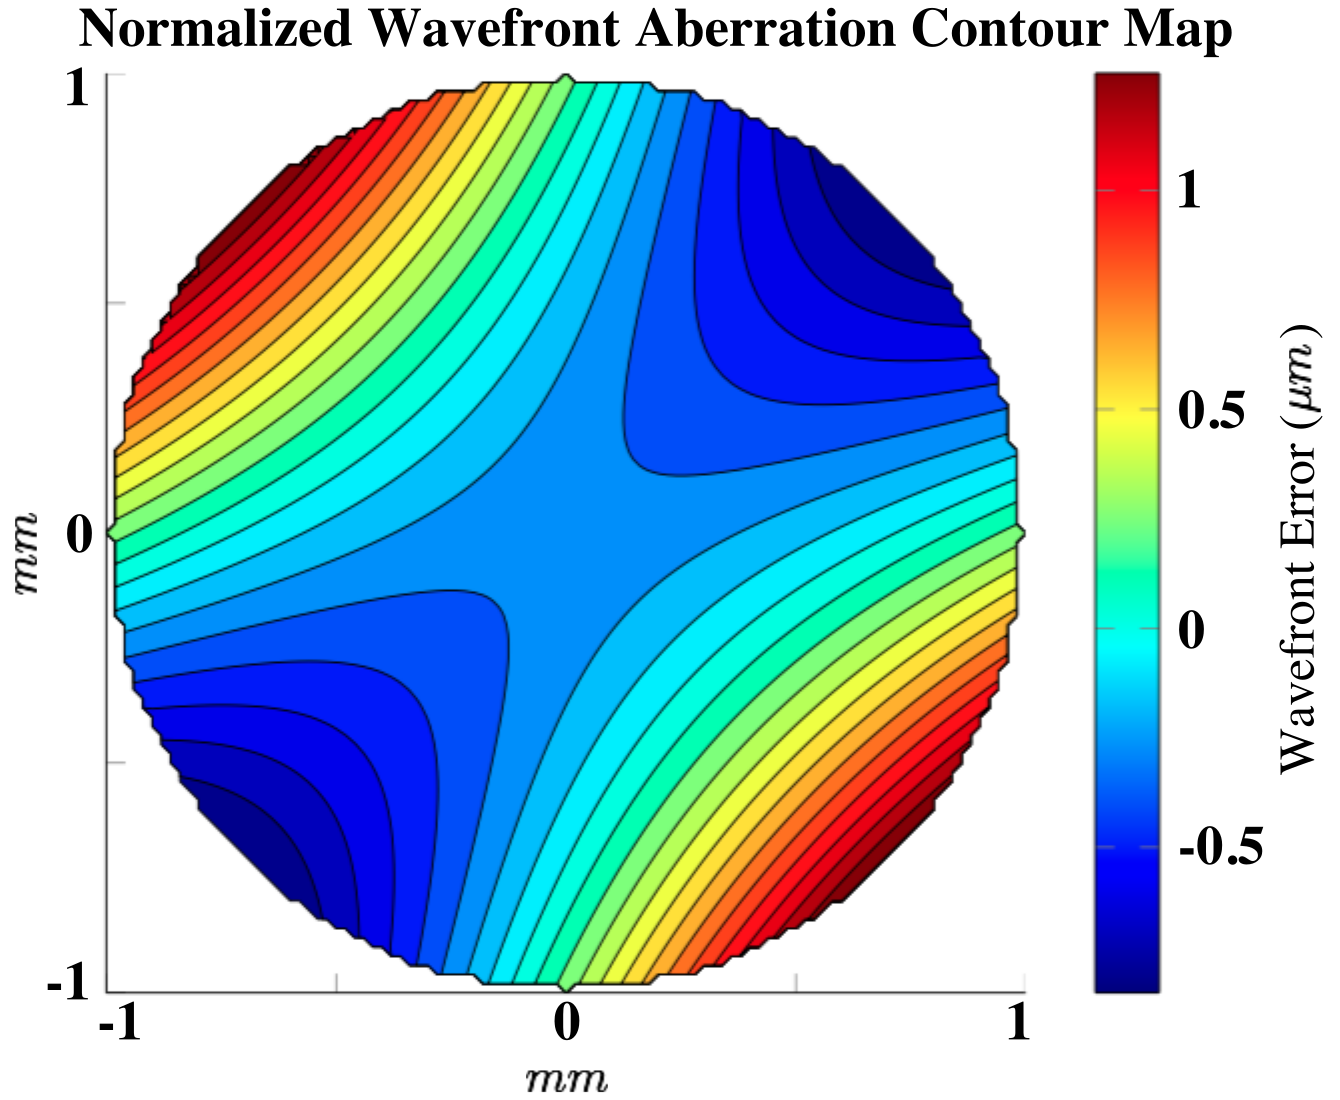
\includegraphics[width=0.70\linewidth]{__Images/04/wavefront.png}
%	\subfigure{
%		\setlength\figureheight{0.45\linewidth} 
%		\setlength\figurewidth{0.6\linewidth} 
%		% This file was created by matlab2tikz.
% Minimal pgfplots version: 1.3
%
%The latest updates can be retrieved from
%  http://www.mathworks.com/matlabcentral/fileexchange/22022-matlab2tikz
%where you can also make suggestions and rate matlab2tikz.
%
\definecolor{mycolor1}{rgb}{0.00000,0.00000,0.56250}%
\definecolor{mycolor2}{rgb}{0.00000,0.00000,0.93750}%
\definecolor{mycolor3}{rgb}{0.00000,0.12500,1.00000}%
\definecolor{mycolor4}{rgb}{0.00000,0.31250,1.00000}%
\definecolor{mycolor5}{rgb}{0.00000,0.56250,1.00000}%
\definecolor{mycolor6}{rgb}{0.00000,0.75000,1.00000}%
\definecolor{mycolor7}{rgb}{0.00000,0.93750,1.00000}%
\definecolor{mycolor8}{rgb}{0.12500,1.00000,0.87500}%
\definecolor{mycolor9}{rgb}{0.31250,1.00000,0.68750}%
\definecolor{mycolor10}{rgb}{0.56250,1.00000,0.43750}%
\definecolor{mycolor11}{rgb}{0.75000,1.00000,0.25000}%
\definecolor{mycolor12}{rgb}{0.93750,1.00000,0.06250}%
\definecolor{mycolor13}{rgb}{1.00000,0.87500,0.00000}%
\definecolor{mycolor14}{rgb}{1.00000,0.06250,0.00000}%
\definecolor{mycolor15}{rgb}{0.87500,0.00000,0.00000}%
\definecolor{mycolor16}{rgb}{0.68750,0.00000,0.00000}%
%
\begin{tikzpicture}

\begin{axis}[%
width=0.75\figurewidth,
height=\figureheight,
at={(0\figurewidth,0\figureheight)},
scale only axis,
every outer x axis line/.append style={black},
every x tick label/.append style={font=\color{black}},
xmin=-1,
xmax=1,
xlabel={mm (right-left)},
every outer y axis line/.append style={black},
every y tick label/.append style={font=\color{black}},
ymin=-1,
ymax=1,
ylabel={mm (superior-inferior)},
title={Normalized Wave Aberration Contour Map},
axis x line*=bottom,
axis y line*=left,
colormap/jet,
colorbar,
colorbar style={separate axis lines,every outer x axis line/.append style={black},every x tick label/.append style={font=\color{black}},every outer y axis line/.append style={black},every y tick label/.append style={font=\color{black}},ylabel={RWMS Error (in microns)}},
point meta min=-0.8325,
point meta max=1.2675
]

\addplot[area legend,solid,fill=mycolor1,draw=black,forget plot]
table[row sep=crcr] {%
x	y\\
-1	1.01015305858709e-06\\
-0.980001030151018	0.02\\
-0.980001070758997	0.04\\
-0.980001111774929	0.0599999999999999\\
-0.980001153198809	0.08\\
-0.980001195030632	0.1\\
-0.980001237270392	0.12\\
-0.980001279918085	0.14\\
-0.980001322973706	0.16\\
-0.980001366437248	0.18\\
-0.98	0.180001366437248\\
-0.960001382353428	0.2\\
-0.960001425816712	0.22\\
-0.960001469687911	0.24\\
-0.960001513967019	0.26\\
-0.960001558654031	0.28\\
-0.96	0.280001558654031\\
-0.94000157212131	0.3\\
-0.940001616808061	0.32\\
-0.940001661902709	0.34\\
-0.94	0.340001661902709\\
-0.920001673737469	0.36\\
-0.92000171883186	0.38\\
-0.92	0.38000171883186\\
-0.900001729442275	0.4\\
-0.900001774536415	0.42\\
-0.9	0.420001774536415\\
-0.8800017839225	0.44\\
-0.880001829016393	0.46\\
-0.88	0.460001829016393\\
-0.860001837178162	0.48\\
-0.860001882271816	0.5\\
-0.86	0.500001882271816\\
-0.840001889209283	0.52\\
-0.840001934302702	0.54\\
-0.84	0.540001934302701\\
-0.82000194001588	0.56\\
-0.82	0.56000194001588\\
-0.800001944912888	0.58\\
-0.800001989597974	0.6\\
-0.8	0.600001989597974\\
-0.780001993270712	0.62\\
-0.78	0.620001993270712\\
-0.760001996127284	0.64\\
-0.76	0.640001996127285\\
-0.740001998167693	0.66\\
-0.74	0.660001998167693\\
-0.720001999391938	0.68\\
-0.72	0.680001999391938\\
-0.70000199980002	0.7\\
-0.7	0.70000199980002\\
-0.680001999391938	0.72\\
-0.68	0.720001999391938\\
-0.660001998167693	0.74\\
-0.66	0.740001998167693\\
-0.640001996127285	0.76\\
-0.64	0.760001996127285\\
-0.620001993270712	0.78\\
-0.62	0.780001993270712\\
-0.600001989597974	0.8\\
-0.6	0.800001989597974\\
-0.58	0.800001944912888\\
-0.56000194001588	0.82\\
-0.56	0.82000194001588\\
-0.540001934302701	0.84\\
-0.54	0.840001934302701\\
-0.52	0.840001889209283\\
-0.500001882271816	0.86\\
-0.5	0.860001882271816\\
-0.48	0.860001837178162\\
-0.460001829016393	0.88\\
-0.46	0.880001829016393\\
-0.44	0.8800017839225\\
-0.420001774536415	0.9\\
-0.42	0.900001774536415\\
-0.4	0.900001729442275\\
-0.38000171883186	0.92\\
-0.38	0.92000171883186\\
-0.36	0.920001673737469\\
-0.340001661902709	0.94\\
-0.34	0.940001661902709\\
-0.32	0.940001616808061\\
-0.3	0.94000157212131\\
-0.280001558654031	0.96\\
-0.28	0.96000155865403\\
-0.26	0.960001513967019\\
-0.24	0.960001469687911\\
-0.22	0.960001425816712\\
-0.2	0.960001382353428\\
-0.180001366437248	0.98\\
-0.18	0.980001366437248\\
-0.16	0.980001322973706\\
-0.14	0.980001279918085\\
-0.12	0.980001237270392\\
-0.1	0.980001195030632\\
-0.08	0.980001153198809\\
-0.0599999999999999	0.980001111774929\\
-0.04	0.980001070758997\\
-0.02	0.980001030151018\\
-1.01015305858709e-06	1\\
0	1.00000101015306\\
1.01015305858709e-06	1\\
0.02	0.98000095015894\\
0.04	0.980000910774849\\
0.0599999999999999	0.980000871798731\\
0.08	0.980000833230591\\
0.1	0.980000795070433\\
0.12	0.980000757318261\\
0.14	0.980000719974081\\
0.16	0.980000683037897\\
0.18	0.980000646509713\\
0.180000646509713	0.98\\
0.2	0.960000598757584\\
0.22	0.960000563861654\\
0.24	0.960000529373743\\
0.26	0.960000495293856\\
0.28	0.960000461621998\\
0.280000461621998	0.96\\
0.3	0.940000421215618\\
0.32	0.940000389176101\\
0.34	0.940000357544628\\
0.340000357544628	0.94\\
0.36	0.920000322035631\\
0.38	0.920000292036552\\
0.380000292036552	0.92\\
0.4	0.900000260200696\\
0.42	0.900000231834047\\
0.420000231834047	0.9\\
0.44	0.880000203671395\\
0.46	0.88000017693721\\
0.46000017693721	0.88\\
0.48	0.860000152447818\\
0.5	0.860000127346128\\
0.500000127346128	0.86\\
0.52	0.840000106530045\\
0.54	0.840000083060879\\
0.54000008306088	0.84\\
0.56	0.82000006591815\\
0.56000006591815	0.82\\
0.58	0.800000051224358\\
0.6	0.800000030612198\\
0.600000030612198	0.8\\
0.62	0.780000019591818\\
0.620000019591818	0.78\\
0.64	0.760000011020402\\
0.640000011020402	0.76\\
0.66	0.740000004897958\\
0.660000004897958	0.74\\
0.68	0.72000000122449\\
0.68000000122449	0.72\\
0.7	0.7\\
0.72	0.68000000122449\\
0.72000000122449	0.68\\
0.74	0.660000004897958\\
0.740000004897958	0.66\\
0.76	0.640000011020402\\
0.760000011020402	0.64\\
0.78	0.620000019591818\\
0.780000019591818	0.62\\
0.8	0.600000030612198\\
0.800000030612198	0.6\\
0.800000051224358	0.58\\
0.82	0.56000006591815\\
0.82000006591815	0.56\\
0.84	0.54000008306088\\
0.840000083060879	0.54\\
0.840000106530045	0.52\\
0.86	0.500000127346128\\
0.860000127346128	0.5\\
0.860000152447818	0.48\\
0.88	0.46000017693721\\
0.88000017693721	0.46\\
0.880000203671395	0.44\\
0.9	0.420000231834047\\
0.900000231834047	0.42\\
0.900000260200696	0.4\\
0.92	0.380000292036552\\
0.920000292036552	0.38\\
0.920000322035631	0.36\\
0.94	0.340000357544628\\
0.940000357544628	0.34\\
0.940000389176101	0.32\\
0.940000421215618	0.3\\
0.96	0.280000461621998\\
0.960000461621998	0.28\\
0.960000495293856	0.26\\
0.960000529373743	0.24\\
0.960000563861654	0.22\\
0.960000598757584	0.2\\
0.98	0.180000646509713\\
0.980000646509713	0.18\\
0.980000683037897	0.16\\
0.980000719974081	0.14\\
0.980000757318261	0.12\\
0.980000795070433	0.1\\
0.980000833230591	0.08\\
0.980000871798731	0.0599999999999999\\
0.980000910774849	0.04\\
0.98000095015894	0.02\\
1	1.01015305858709e-06\\
1.00000101015306	0\\
1	-1.01015305858709e-06\\
0.980001030151018	-0.02\\
0.980001070758997	-0.04\\
0.980001111774929	-0.0599999999999999\\
0.980001153198809	-0.08\\
0.980001195030632	-0.1\\
0.980001237270392	-0.12\\
0.980001279918085	-0.14\\
0.980001322973706	-0.16\\
0.980001366437248	-0.18\\
0.98	-0.180001366437248\\
0.960001382353428	-0.2\\
0.960001425816712	-0.22\\
0.960001469687911	-0.24\\
0.960001513967019	-0.26\\
0.96000155865403	-0.28\\
0.96	-0.280001558654031\\
0.94000157212131	-0.3\\
0.940001616808061	-0.32\\
0.940001661902709	-0.34\\
0.94	-0.340001661902709\\
0.920001673737469	-0.36\\
0.92000171883186	-0.38\\
0.92	-0.38000171883186\\
0.900001729442275	-0.4\\
0.900001774536415	-0.42\\
0.9	-0.420001774536415\\
0.8800017839225	-0.44\\
0.880001829016393	-0.46\\
0.88	-0.460001829016393\\
0.860001837178162	-0.48\\
0.860001882271816	-0.5\\
0.86	-0.500001882271816\\
0.840001889209283	-0.52\\
0.840001934302701	-0.54\\
0.84	-0.540001934302701\\
0.82000194001588	-0.56\\
0.82	-0.56000194001588\\
0.800001944912888	-0.58\\
0.800001989597974	-0.6\\
0.8	-0.600001989597974\\
0.780001993270712	-0.62\\
0.78	-0.620001993270712\\
0.760001996127285	-0.64\\
0.76	-0.640001996127285\\
0.740001998167693	-0.66\\
0.74	-0.660001998167693\\
0.720001999391938	-0.68\\
0.72	-0.680001999391938\\
0.70000199980002	-0.7\\
0.7	-0.70000199980002\\
0.680001999391938	-0.72\\
0.68	-0.720001999391938\\
0.660001998167693	-0.74\\
0.66	-0.740001998167693\\
0.640001996127285	-0.76\\
0.64	-0.760001996127284\\
0.620001993270712	-0.78\\
0.62	-0.780001993270712\\
0.600001989597974	-0.8\\
0.6	-0.800001989597974\\
0.58	-0.800001944912888\\
0.56000194001588	-0.82\\
0.56	-0.82000194001588\\
0.540001934302701	-0.84\\
0.54	-0.840001934302702\\
0.52	-0.840001889209283\\
0.500001882271816	-0.86\\
0.5	-0.860001882271816\\
0.48	-0.860001837178162\\
0.460001829016393	-0.88\\
0.46	-0.880001829016393\\
0.44	-0.8800017839225\\
0.420001774536415	-0.9\\
0.42	-0.900001774536415\\
0.4	-0.900001729442275\\
0.38000171883186	-0.92\\
0.38	-0.92000171883186\\
0.36	-0.920001673737469\\
0.340001661902709	-0.94\\
0.34	-0.940001661902709\\
0.32	-0.940001616808061\\
0.3	-0.94000157212131\\
0.280001558654031	-0.96\\
0.28	-0.960001558654031\\
0.26	-0.960001513967019\\
0.24	-0.960001469687911\\
0.22	-0.960001425816712\\
0.2	-0.960001382353428\\
0.180001366437248	-0.98\\
0.18	-0.980001366437248\\
0.16	-0.980001322973706\\
0.14	-0.980001279918085\\
0.12	-0.980001237270392\\
0.1	-0.980001195030632\\
0.08	-0.980001153198809\\
0.0599999999999999	-0.980001111774929\\
0.04	-0.980001070758997\\
0.02	-0.980001030151018\\
1.01015305858709e-06	-1\\
0	-1.00000101015306\\
-1.01015305858709e-06	-1\\
-0.02	-0.980000950158939\\
-0.04	-0.980000910774849\\
-0.0599999999999999	-0.980000871798731\\
-0.08	-0.980000833230591\\
-0.1	-0.980000795070433\\
-0.12	-0.980000757318261\\
-0.14	-0.980000719974081\\
-0.16	-0.980000683037897\\
-0.18	-0.980000646509713\\
-0.180000646509713	-0.98\\
-0.2	-0.960000598757584\\
-0.22	-0.960000563861654\\
-0.24	-0.960000529373743\\
-0.26	-0.960000495293856\\
-0.28	-0.960000461621998\\
-0.280000461621998	-0.96\\
-0.3	-0.940000421215618\\
-0.32	-0.9400003891761\\
-0.34	-0.940000357544628\\
-0.340000357544628	-0.94\\
-0.36	-0.920000322035631\\
-0.38	-0.920000292036552\\
-0.380000292036552	-0.92\\
-0.4	-0.900000260200696\\
-0.42	-0.900000231834047\\
-0.420000231834047	-0.9\\
-0.44	-0.880000203671395\\
-0.46	-0.88000017693721\\
-0.46000017693721	-0.88\\
-0.48	-0.860000152447818\\
-0.5	-0.860000127346128\\
-0.500000127346128	-0.86\\
-0.52	-0.840000106530045\\
-0.54	-0.840000083060879\\
-0.54000008306088	-0.84\\
-0.56	-0.82000006591815\\
-0.56000006591815	-0.82\\
-0.58	-0.800000051224359\\
-0.6	-0.800000030612198\\
-0.600000030612198	-0.8\\
-0.62	-0.780000019591818\\
-0.620000019591817	-0.78\\
-0.64	-0.760000011020402\\
-0.640000011020402	-0.76\\
-0.66	-0.740000004897958\\
-0.660000004897958	-0.74\\
-0.68	-0.72000000122449\\
-0.68000000122449	-0.72\\
-0.7	-0.7\\
-0.72	-0.68000000122449\\
-0.72000000122449	-0.68\\
-0.74	-0.660000004897958\\
-0.740000004897958	-0.66\\
-0.76	-0.640000011020402\\
-0.760000011020402	-0.64\\
-0.78	-0.620000019591817\\
-0.780000019591818	-0.62\\
-0.8	-0.600000030612198\\
-0.800000030612198	-0.6\\
-0.800000051224359	-0.58\\
-0.82	-0.56000006591815\\
-0.82000006591815	-0.56\\
-0.84	-0.54000008306088\\
-0.840000083060879	-0.54\\
-0.840000106530045	-0.52\\
-0.86	-0.500000127346128\\
-0.860000127346128	-0.5\\
-0.860000152447818	-0.48\\
-0.88	-0.46000017693721\\
-0.88000017693721	-0.46\\
-0.880000203671395	-0.44\\
-0.9	-0.420000231834047\\
-0.900000231834047	-0.42\\
-0.900000260200696	-0.4\\
-0.92	-0.380000292036552\\
-0.920000292036552	-0.38\\
-0.920000322035631	-0.36\\
-0.94	-0.340000357544628\\
-0.940000357544628	-0.34\\
-0.9400003891761	-0.32\\
-0.940000421215618	-0.3\\
-0.96	-0.280000461621998\\
-0.960000461621998	-0.28\\
-0.960000495293856	-0.26\\
-0.960000529373743	-0.24\\
-0.960000563861654	-0.22\\
-0.960000598757584	-0.2\\
-0.98	-0.180000646509713\\
-0.980000646509713	-0.18\\
-0.980000683037897	-0.16\\
-0.980000719974081	-0.14\\
-0.980000757318261	-0.12\\
-0.980000795070433	-0.1\\
-0.980000833230591	-0.08\\
-0.980000871798731	-0.0599999999999999\\
-0.980000910774849	-0.04\\
-0.980000950158939	-0.02\\
-1	-1.01015305858709e-06\\
-1.00000101015306	0\\
-1	1.01015305858709e-06\\
}--cycle;


\addplot[area legend,solid,fill=black!25!blue,draw=black,forget plot]
table[row sep=crcr] {%
x	y\\
-1	9.1491977357805e-07\\
-0.980000934917829	0.02\\
-0.980000975526001	0.04\\
-0.980001016542128	0.0599999999999999\\
-0.980001057966205	0.08\\
-0.980001099798227	0.1\\
-0.980001142038189	0.12\\
-0.980001184686085	0.14\\
-0.98000122774191	0.16\\
-0.98000127120566	0.18\\
-0.98	0.18000127120566\\
-0.960001287121915	0.2\\
-0.960001330585407	0.22\\
-0.960001374456815	0.24\\
-0.960001418736133	0.26\\
-0.960001463423358	0.28\\
-0.96	0.280001463423358\\
-0.940001476890701	0.3\\
-0.940001521577665	0.32\\
-0.940001566672527	0.34\\
-0.94	0.340001566672527\\
-0.920001578507344	0.36\\
-0.92000162360195	0.38\\
-0.92	0.38000162360195\\
-0.900001634212416	0.4\\
-0.90000167930677	0.42\\
-0.9	0.42000167930677\\
-0.880001688692899	0.44\\
-0.880001733787008	0.46\\
-0.88	0.460001733787007\\
-0.860001741948815	0.48\\
-0.860001787042683	0.5\\
-0.86	0.500001787042684\\
-0.840001793980184	0.52\\
-0.840001839073817	0.54\\
-0.84	0.540001839073817\\
-0.820001844787023	0.56\\
-0.82	0.560001844787023\\
-0.800001849684055	0.58\\
-0.800001894369353	0.6\\
-0.8	0.600001894369353\\
-0.780001898042108	0.62\\
-0.78	0.620001898042108\\
-0.760001900898695	0.64\\
-0.76	0.640001900898695\\
-0.740001902939113	0.66\\
-0.74	0.660001902939113\\
-0.720001904163364	0.68\\
-0.72	0.680001904163364\\
-0.700001904571448	0.7\\
-0.7	0.700001904571448\\
-0.680001904163364	0.72\\
-0.68	0.720001904163364\\
-0.660001902939113	0.74\\
-0.66	0.740001902939113\\
-0.640001900898695	0.76\\
-0.64	0.760001900898695\\
-0.620001898042108	0.78\\
-0.62	0.780001898042108\\
-0.600001894369353	0.8\\
-0.6	0.800001894369353\\
-0.58	0.800001849684055\\
-0.560001844787023	0.82\\
-0.56	0.820001844787023\\
-0.540001839073817	0.84\\
-0.54	0.840001839073817\\
-0.52	0.840001793980183\\
-0.500001787042683	0.86\\
-0.5	0.860001787042684\\
-0.48	0.860001741948815\\
-0.460001733787007	0.88\\
-0.46	0.880001733787007\\
-0.44	0.880001688692899\\
-0.42000167930677	0.9\\
-0.42	0.900001679306769\\
-0.4	0.900001634212416\\
-0.38000162360195	0.92\\
-0.38	0.92000162360195\\
-0.36	0.920001578507344\\
-0.340001566672527	0.94\\
-0.34	0.940001566672527\\
-0.32	0.940001521577665\\
-0.3	0.940001476890701\\
-0.280001463423358	0.96\\
-0.28	0.960001463423358\\
-0.26	0.960001418736133\\
-0.24	0.960001374456814\\
-0.22	0.960001330585407\\
-0.2	0.960001287121915\\
-0.18000127120566	0.98\\
-0.18	0.98000127120566\\
-0.16	0.98000122774191\\
-0.14	0.980001184686085\\
-0.12	0.980001142038189\\
-0.1	0.980001099798227\\
-0.08	0.980001057966205\\
-0.0599999999999999	0.980001016542128\\
-0.04	0.980000975526001\\
-0.02	0.980000934917828\\
-9.1491977357805e-07	1\\
0	1.00000091491977\\
9.1491977357805e-07	1\\
0.02	0.980000854925369\\
0.04	0.980000815541091\\
0.0599999999999999	0.980000776564788\\
0.08	0.980000737996463\\
0.1	0.980000699836123\\
0.12	0.980000662083772\\
0.14	0.980000624739414\\
0.16	0.980000587803054\\
0.18	0.980000551274696\\
0.180000551274696	0.98\\
0.2	0.96000050352234\\
0.22	0.960000468626243\\
0.24	0.960000434138168\\
0.26	0.96000040005812\\
0.28	0.960000366386101\\
0.280000366386101	0.96\\
0.3	0.940000325979529\\
0.32	0.940000293939858\\
0.34	0.940000262308236\\
0.340000262308236	0.94\\
0.36	0.920000226799069\\
0.38	0.920000196799847\\
0.380000196799847	0.92\\
0.4	0.90000016496384\\
0.42	0.900000136597056\\
0.420000136597056	0.9\\
0.44	0.88000010843427\\
0.46	0.880000081699957\\
0.460000081699957	0.88\\
0.48	0.860000057210448\\
0.5	0.860000032108639\\
0.500000032108639	0.86\\
0.52	0.840000011292457\\
0.529623188405797	0.84\\
0.533753753753754	0.82\\
0.538566978193146	0.8\\
0.54	0.794712643678161\\
0.544224422442244	0.78\\
0.550790378006873	0.76\\
0.558351254480287	0.74\\
0.56	0.736068376068376\\
0.5672030651341	0.72\\
0.577429718875502	0.7\\
0.58	0.695460992907801\\
0.589437229437229	0.68\\
0.6	0.664654088050314\\
0.603474178403756	0.66\\
0.62	0.640112994350282\\
0.620102564102564	0.64\\
0.64	0.620102564102564\\
0.640112994350282	0.62\\
0.66	0.603474178403756\\
0.664654088050314	0.6\\
0.68	0.589437229437229\\
0.695460992907801	0.58\\
0.7	0.577429718875502\\
0.72	0.5672030651341\\
0.736068376068376	0.56\\
0.74	0.558351254480287\\
0.76	0.550790378006873\\
0.78	0.544224422442244\\
0.79471264367816	0.54\\
0.8	0.538566978193146\\
0.82	0.533753753753754\\
0.84	0.529623188405797\\
0.840000011292457	0.52\\
0.86	0.500000032108639\\
0.860000032108639	0.5\\
0.860000057210448	0.48\\
0.88	0.460000081699957\\
0.880000081699957	0.46\\
0.88000010843427	0.44\\
0.9	0.420000136597056\\
0.900000136597056	0.42\\
0.90000016496384	0.4\\
0.92	0.380000196799847\\
0.920000196799847	0.38\\
0.920000226799069	0.36\\
0.94	0.340000262308236\\
0.940000262308236	0.34\\
0.940000293939858	0.32\\
0.940000325979529	0.3\\
0.96	0.280000366386101\\
0.960000366386101	0.28\\
0.96000040005812	0.26\\
0.960000434138168	0.24\\
0.960000468626243	0.22\\
0.96000050352234	0.2\\
0.98	0.180000551274696\\
0.980000551274696	0.18\\
0.980000587803054	0.16\\
0.980000624739414	0.14\\
0.980000662083772	0.12\\
0.980000699836123	0.1\\
0.980000737996463	0.08\\
0.980000776564788	0.0599999999999999\\
0.980000815541091	0.04\\
0.980000854925369	0.02\\
1	9.1491977357805e-07\\
1.00000091491977	0\\
1	-9.1491977357805e-07\\
0.980000934917828	-0.02\\
0.980000975526001	-0.04\\
0.980001016542128	-0.0599999999999999\\
0.980001057966205	-0.08\\
0.980001099798227	-0.1\\
0.980001142038189	-0.12\\
0.980001184686085	-0.14\\
0.98000122774191	-0.16\\
0.98000127120566	-0.18\\
0.98	-0.18000127120566\\
0.960001287121915	-0.2\\
0.960001330585407	-0.22\\
0.960001374456814	-0.24\\
0.960001418736133	-0.26\\
0.960001463423358	-0.28\\
0.96	-0.280001463423358\\
0.940001476890701	-0.3\\
0.940001521577665	-0.32\\
0.940001566672527	-0.34\\
0.94	-0.340001566672527\\
0.920001578507344	-0.36\\
0.92000162360195	-0.38\\
0.92	-0.38000162360195\\
0.900001634212416	-0.4\\
0.900001679306769	-0.42\\
0.9	-0.42000167930677\\
0.880001688692899	-0.44\\
0.880001733787007	-0.46\\
0.88	-0.460001733787007\\
0.860001741948815	-0.48\\
0.860001787042684	-0.5\\
0.86	-0.500001787042683\\
0.840001793980183	-0.52\\
0.840001839073817	-0.54\\
0.84	-0.540001839073817\\
0.820001844787023	-0.56\\
0.82	-0.560001844787023\\
0.800001849684055	-0.58\\
0.800001894369353	-0.6\\
0.8	-0.600001894369353\\
0.780001898042108	-0.62\\
0.78	-0.620001898042108\\
0.760001900898695	-0.64\\
0.76	-0.640001900898695\\
0.740001902939113	-0.66\\
0.74	-0.660001902939113\\
0.720001904163364	-0.68\\
0.72	-0.680001904163364\\
0.700001904571448	-0.7\\
0.7	-0.700001904571448\\
0.680001904163364	-0.72\\
0.68	-0.720001904163364\\
0.660001902939113	-0.74\\
0.66	-0.740001902939113\\
0.640001900898695	-0.76\\
0.64	-0.760001900898695\\
0.620001898042108	-0.78\\
0.62	-0.780001898042108\\
0.600001894369353	-0.8\\
0.6	-0.800001894369353\\
0.58	-0.800001849684054\\
0.560001844787023	-0.82\\
0.56	-0.820001844787023\\
0.540001839073817	-0.84\\
0.54	-0.840001839073817\\
0.52	-0.840001793980184\\
0.500001787042684	-0.86\\
0.5	-0.860001787042683\\
0.48	-0.860001741948815\\
0.460001733787007	-0.88\\
0.46	-0.880001733787008\\
0.44	-0.880001688692899\\
0.42000167930677	-0.9\\
0.42	-0.90000167930677\\
0.4	-0.900001634212416\\
0.38000162360195	-0.92\\
0.38	-0.92000162360195\\
0.36	-0.920001578507344\\
0.340001566672527	-0.94\\
0.34	-0.940001566672527\\
0.32	-0.940001521577665\\
0.3	-0.940001476890701\\
0.280001463423358	-0.96\\
0.28	-0.960001463423358\\
0.26	-0.960001418736133\\
0.24	-0.960001374456815\\
0.22	-0.960001330585407\\
0.2	-0.960001287121915\\
0.18000127120566	-0.98\\
0.18	-0.98000127120566\\
0.16	-0.98000122774191\\
0.14	-0.980001184686085\\
0.12	-0.980001142038189\\
0.1	-0.980001099798227\\
0.08	-0.980001057966205\\
0.0599999999999999	-0.980001016542128\\
0.04	-0.980000975526001\\
0.02	-0.980000934917829\\
9.1491977357805e-07	-1\\
0	-1.00000091491977\\
-9.1491977357805e-07	-1\\
-0.02	-0.980000854925369\\
-0.04	-0.980000815541091\\
-0.0599999999999999	-0.980000776564788\\
-0.08	-0.980000737996463\\
-0.1	-0.980000699836123\\
-0.12	-0.980000662083772\\
-0.14	-0.980000624739414\\
-0.16	-0.980000587803054\\
-0.18	-0.980000551274696\\
-0.180000551274696	-0.98\\
-0.2	-0.96000050352234\\
-0.22	-0.960000468626243\\
-0.24	-0.960000434138168\\
-0.26	-0.96000040005812\\
-0.28	-0.960000366386101\\
-0.280000366386101	-0.96\\
-0.3	-0.940000325979529\\
-0.32	-0.940000293939858\\
-0.34	-0.940000262308236\\
-0.340000262308236	-0.94\\
-0.36	-0.920000226799069\\
-0.38	-0.920000196799847\\
-0.380000196799847	-0.92\\
-0.4	-0.90000016496384\\
-0.42	-0.900000136597056\\
-0.420000136597056	-0.9\\
-0.44	-0.88000010843427\\
-0.46	-0.880000081699957\\
-0.460000081699957	-0.88\\
-0.48	-0.860000057210448\\
-0.5	-0.860000032108639\\
-0.500000032108639	-0.86\\
-0.52	-0.840000011292457\\
-0.529623188405797	-0.84\\
-0.533753753753754	-0.82\\
-0.538566978193146	-0.8\\
-0.54	-0.794712643678161\\
-0.544224422442244	-0.78\\
-0.550790378006873	-0.76\\
-0.558351254480287	-0.74\\
-0.56	-0.736068376068376\\
-0.5672030651341	-0.72\\
-0.577429718875502	-0.7\\
-0.58	-0.695460992907801\\
-0.589437229437229	-0.68\\
-0.6	-0.664654088050314\\
-0.603474178403756	-0.66\\
-0.62	-0.640112994350282\\
-0.620102564102564	-0.64\\
-0.64	-0.620102564102564\\
-0.640112994350282	-0.62\\
-0.66	-0.603474178403756\\
-0.664654088050314	-0.6\\
-0.68	-0.589437229437229\\
-0.695460992907801	-0.58\\
-0.7	-0.577429718875502\\
-0.72	-0.5672030651341\\
-0.736068376068376	-0.56\\
-0.74	-0.558351254480287\\
-0.76	-0.550790378006873\\
-0.78	-0.544224422442244\\
-0.79471264367816	-0.54\\
-0.8	-0.538566978193146\\
-0.82	-0.533753753753754\\
-0.84	-0.529623188405797\\
-0.840000011292457	-0.52\\
-0.86	-0.500000032108639\\
-0.860000032108639	-0.5\\
-0.860000057210448	-0.48\\
-0.88	-0.460000081699957\\
-0.880000081699957	-0.46\\
-0.88000010843427	-0.44\\
-0.9	-0.420000136597056\\
-0.900000136597056	-0.42\\
-0.90000016496384	-0.4\\
-0.92	-0.380000196799847\\
-0.920000196799847	-0.38\\
-0.920000226799069	-0.36\\
-0.94	-0.340000262308236\\
-0.940000262308236	-0.34\\
-0.940000293939858	-0.32\\
-0.940000325979529	-0.3\\
-0.96	-0.280000366386101\\
-0.960000366386101	-0.28\\
-0.96000040005812	-0.26\\
-0.960000434138168	-0.24\\
-0.960000468626243	-0.22\\
-0.96000050352234	-0.2\\
-0.98	-0.180000551274696\\
-0.980000551274696	-0.18\\
-0.980000587803054	-0.16\\
-0.980000624739414	-0.14\\
-0.980000662083772	-0.12\\
-0.980000699836123	-0.1\\
-0.980000737996463	-0.08\\
-0.980000776564788	-0.0599999999999999\\
-0.980000815541091	-0.04\\
-0.980000854925369	-0.02\\
-1	-9.1491977357805e-07\\
-1.00000091491977	0\\
-1	9.1491977357805e-07\\
}--cycle;


\addplot[area legend,solid,fill=mycolor2,draw=black,forget plot]
table[row sep=crcr] {%
x	y\\
-1	8.19686488569005e-07\\
-0.980000839684639	0.02\\
-0.980000880293004	0.04\\
-0.980000921309327	0.0599999999999999\\
-0.980000962733601	0.08\\
-0.980001004565822	0.1\\
-0.980001046805985	0.12\\
-0.980001089454084	0.14\\
-0.980001132510115	0.16\\
-0.980001175974072	0.18\\
-0.98	0.180001175974071\\
-0.960001191890403	0.2\\
-0.960001235354101	0.22\\
-0.960001279225718	0.24\\
-0.960001323505247	0.26\\
-0.960001368192684	0.28\\
-0.96	0.280001368192685\\
-0.940001381660092	0.3\\
-0.940001426347269	0.32\\
-0.940001471442346	0.34\\
-0.94	0.340001471442346\\
-0.920001483277219	0.36\\
-0.920001528372039	0.38\\
-0.92	0.380001528372039\\
-0.900001538982556	0.4\\
-0.900001584077124	0.42\\
-0.9	0.420001584077125\\
-0.880001593463299	0.44\\
-0.880001638557622	0.46\\
-0.88	0.460001638557622\\
-0.860001646719468	0.48\\
-0.860001691813551	0.5\\
-0.86	0.500001691813551\\
-0.840001698751085	0.52\\
-0.840001743844933	0.54\\
-0.84	0.540001743844933\\
-0.820001749558166	0.56\\
-0.82	0.560001749558166\\
-0.800001754455221	0.58\\
-0.800001799140732	0.6\\
-0.8	0.600001799140732\\
-0.780001802813505	0.62\\
-0.78	0.620001802813505\\
-0.760001805670105	0.64\\
-0.76	0.640001805670105\\
-0.740001807710533	0.66\\
-0.74	0.660001807710533\\
-0.72000180893479	0.68\\
-0.72	0.68000180893479\\
-0.700001809342875	0.7\\
-0.7	0.700001809342875\\
-0.68000180893479	0.72\\
-0.68	0.72000180893479\\
-0.660001807710533	0.74\\
-0.66	0.740001807710533\\
-0.640001805670105	0.76\\
-0.64	0.760001805670105\\
-0.620001802813505	0.78\\
-0.62	0.780001802813505\\
-0.600001799140732	0.8\\
-0.6	0.800001799140732\\
-0.58	0.800001754455221\\
-0.560001749558166	0.82\\
-0.56	0.820001749558166\\
-0.540001743844933	0.84\\
-0.54	0.840001743844933\\
-0.52	0.840001698751085\\
-0.500001691813551	0.86\\
-0.5	0.860001691813551\\
-0.48	0.860001646719469\\
-0.460001638557622	0.88\\
-0.46	0.880001638557622\\
-0.44	0.880001593463299\\
-0.420001584077125	0.9\\
-0.42	0.900001584077125\\
-0.4	0.900001538982556\\
-0.380001528372039	0.92\\
-0.38	0.920001528372039\\
-0.36	0.920001483277219\\
-0.340001471442346	0.94\\
-0.34	0.940001471442346\\
-0.32	0.940001426347269\\
-0.3	0.940001381660092\\
-0.280001368192685	0.96\\
-0.28	0.960001368192684\\
-0.26	0.960001323505247\\
-0.24	0.960001279225718\\
-0.22	0.960001235354101\\
-0.2	0.960001191890403\\
-0.180001175974071	0.98\\
-0.18	0.980001175974072\\
-0.16	0.980001132510115\\
-0.14	0.980001089454084\\
-0.12	0.980001046805985\\
-0.1	0.980001004565822\\
-0.08	0.980000962733601\\
-0.0599999999999999	0.980000921309327\\
-0.04	0.980000880293005\\
-0.02	0.980000839684639\\
-8.19686488569005e-07	1\\
0	1.00000081968649\\
8.19686488569005e-07	1\\
0.02	0.980000759691798\\
0.04	0.980000720307333\\
0.0599999999999999	0.980000681330844\\
0.08	0.980000642762336\\
0.1	0.980000604601814\\
0.12	0.980000566849283\\
0.14	0.980000529504747\\
0.16	0.980000492568211\\
0.18	0.980000456039679\\
0.18000045603968	0.98\\
0.2	0.960000408287096\\
0.22	0.960000373390833\\
0.24	0.960000338902594\\
0.26	0.960000304822383\\
0.28	0.960000271150204\\
0.280000271150204	0.96\\
0.3	0.94000023074344\\
0.32	0.940000198703616\\
0.34	0.940000167071843\\
0.340000167071843	0.94\\
0.36	0.920000131562507\\
0.38	0.920000101563143\\
0.380000101563143	0.92\\
0.4	0.900000069726984\\
0.42	0.900000041360065\\
0.420000041360065	0.9\\
0.44	0.880000013197144\\
0.449872773536896	0.88\\
0.450341207349082	0.86\\
0.451165311653116	0.84\\
0.452380952380952	0.82\\
0.454028985507246	0.8\\
0.456156156156156	0.78\\
0.458816199376947	0.76\\
0.46	0.752549019607843\\
0.462112211221122	0.74\\
0.466116838487972	0.72\\
0.47089605734767	0.7\\
0.476554307116105	0.68\\
0.48	0.669425287356321\\
0.483293172690763	0.66\\
0.491308016877637	0.64\\
0.5	0.621441441441441\\
0.500730593607306	0.62\\
0.51207729468599	0.6\\
0.52	0.587851851851852\\
0.525608465608466	0.58\\
0.54	0.562222222222222\\
0.541988304093567	0.56\\
0.56	0.541988304093567\\
0.562222222222222	0.54\\
0.58	0.525608465608466\\
0.587851851851852	0.52\\
0.6	0.51207729468599\\
0.62	0.500730593607306\\
0.621441441441441	0.5\\
0.64	0.491308016877637\\
0.66	0.483293172690763\\
0.669425287356321	0.48\\
0.68	0.476554307116105\\
0.7	0.47089605734767\\
0.72	0.466116838487972\\
0.74	0.462112211221122\\
0.752549019607843	0.46\\
0.76	0.458816199376947\\
0.78	0.456156156156156\\
0.8	0.454028985507246\\
0.82	0.452380952380952\\
0.84	0.451165311653116\\
0.86	0.450341207349081\\
0.88	0.449872773536896\\
0.880000013197144	0.44\\
0.9	0.420000041360065\\
0.900000041360065	0.42\\
0.900000069726984	0.4\\
0.92	0.380000101563143\\
0.920000101563143	0.38\\
0.920000131562507	0.36\\
0.94	0.340000167071843\\
0.940000167071843	0.34\\
0.940000198703616	0.32\\
0.94000023074344	0.3\\
0.96	0.280000271150204\\
0.960000271150204	0.28\\
0.960000304822383	0.26\\
0.960000338902594	0.24\\
0.960000373390833	0.22\\
0.960000408287096	0.2\\
0.98	0.18000045603968\\
0.980000456039679	0.18\\
0.980000492568211	0.16\\
0.980000529504747	0.14\\
0.980000566849283	0.12\\
0.980000604601814	0.1\\
0.980000642762336	0.08\\
0.980000681330844	0.0599999999999999\\
0.980000720307333	0.04\\
0.980000759691798	0.02\\
1	8.19686488569005e-07\\
1.00000081968649	0\\
1	-8.19686488569005e-07\\
0.980000839684639	-0.02\\
0.980000880293005	-0.04\\
0.980000921309327	-0.0599999999999999\\
0.980000962733601	-0.08\\
0.980001004565822	-0.1\\
0.980001046805985	-0.12\\
0.980001089454084	-0.14\\
0.980001132510115	-0.16\\
0.980001175974072	-0.18\\
0.98	-0.180001175974071\\
0.960001191890403	-0.2\\
0.960001235354101	-0.22\\
0.960001279225718	-0.24\\
0.960001323505247	-0.26\\
0.960001368192684	-0.28\\
0.96	-0.280001368192685\\
0.940001381660092	-0.3\\
0.940001426347269	-0.32\\
0.940001471442346	-0.34\\
0.94	-0.340001471442346\\
0.920001483277219	-0.36\\
0.920001528372039	-0.38\\
0.92	-0.380001528372039\\
0.900001538982556	-0.4\\
0.900001584077124	-0.42\\
0.9	-0.420001584077125\\
0.880001593463299	-0.44\\
0.880001638557622	-0.46\\
0.88	-0.460001638557622\\
0.860001646719469	-0.48\\
0.860001691813551	-0.5\\
0.86	-0.500001691813551\\
0.840001698751085	-0.52\\
0.840001743844933	-0.54\\
0.84	-0.540001743844933\\
0.820001749558166	-0.56\\
0.82	-0.560001749558166\\
0.800001754455221	-0.58\\
0.800001799140732	-0.6\\
0.8	-0.600001799140732\\
0.780001802813505	-0.62\\
0.78	-0.620001802813505\\
0.760001805670105	-0.64\\
0.76	-0.640001805670105\\
0.740001807710533	-0.66\\
0.74	-0.660001807710533\\
0.72000180893479	-0.68\\
0.72	-0.68000180893479\\
0.700001809342875	-0.7\\
0.7	-0.700001809342875\\
0.68000180893479	-0.72\\
0.68	-0.72000180893479\\
0.660001807710533	-0.74\\
0.66	-0.740001807710533\\
0.640001805670105	-0.76\\
0.64	-0.760001805670105\\
0.620001802813505	-0.78\\
0.62	-0.780001802813505\\
0.600001799140732	-0.8\\
0.6	-0.800001799140732\\
0.58	-0.800001754455221\\
0.560001749558166	-0.82\\
0.56	-0.820001749558166\\
0.540001743844933	-0.84\\
0.54	-0.840001743844933\\
0.52	-0.840001698751085\\
0.500001691813551	-0.86\\
0.5	-0.860001691813551\\
0.48	-0.860001646719468\\
0.460001638557622	-0.88\\
0.46	-0.880001638557622\\
0.44	-0.880001593463299\\
0.420001584077124	-0.9\\
0.42	-0.900001584077124\\
0.4	-0.900001538982556\\
0.380001528372039	-0.92\\
0.38	-0.920001528372039\\
0.36	-0.920001483277219\\
0.340001471442346	-0.94\\
0.34	-0.940001471442346\\
0.32	-0.940001426347269\\
0.3	-0.940001381660092\\
0.280001368192685	-0.96\\
0.28	-0.960001368192684\\
0.26	-0.960001323505247\\
0.24	-0.960001279225718\\
0.22	-0.960001235354101\\
0.2	-0.960001191890403\\
0.180001175974071	-0.98\\
0.18	-0.980001175974072\\
0.16	-0.980001132510115\\
0.14	-0.980001089454084\\
0.12	-0.980001046805985\\
0.1	-0.980001004565822\\
0.08	-0.980000962733601\\
0.0599999999999999	-0.980000921309327\\
0.04	-0.980000880293004\\
0.02	-0.980000839684639\\
8.19686488569005e-07	-1\\
0	-1.00000081968649\\
-8.19686488569005e-07	-1\\
-0.02	-0.980000759691798\\
-0.04	-0.980000720307333\\
-0.0599999999999999	-0.980000681330844\\
-0.08	-0.980000642762336\\
-0.1	-0.980000604601814\\
-0.12	-0.980000566849283\\
-0.14	-0.980000529504747\\
-0.16	-0.980000492568211\\
-0.18	-0.98000045603968\\
-0.18000045603968	-0.98\\
-0.2	-0.960000408287096\\
-0.22	-0.960000373390833\\
-0.24	-0.960000338902594\\
-0.26	-0.960000304822383\\
-0.28	-0.960000271150204\\
-0.280000271150204	-0.96\\
-0.3	-0.94000023074344\\
-0.32	-0.940000198703616\\
-0.34	-0.940000167071843\\
-0.340000167071843	-0.94\\
-0.36	-0.920000131562507\\
-0.38	-0.920000101563143\\
-0.380000101563143	-0.92\\
-0.4	-0.900000069726984\\
-0.42	-0.900000041360065\\
-0.420000041360065	-0.9\\
-0.44	-0.880000013197144\\
-0.449872773536896	-0.88\\
-0.450341207349081	-0.86\\
-0.451165311653116	-0.84\\
-0.452380952380952	-0.82\\
-0.454028985507246	-0.8\\
-0.456156156156156	-0.78\\
-0.458816199376947	-0.76\\
-0.46	-0.752549019607843\\
-0.462112211221122	-0.74\\
-0.466116838487972	-0.72\\
-0.47089605734767	-0.7\\
-0.476554307116105	-0.68\\
-0.48	-0.669425287356321\\
-0.483293172690763	-0.66\\
-0.491308016877637	-0.64\\
-0.5	-0.621441441441441\\
-0.500730593607306	-0.62\\
-0.51207729468599	-0.6\\
-0.52	-0.587851851851852\\
-0.525608465608466	-0.58\\
-0.54	-0.562222222222222\\
-0.541988304093567	-0.56\\
-0.56	-0.541988304093567\\
-0.562222222222222	-0.54\\
-0.58	-0.525608465608466\\
-0.587851851851852	-0.52\\
-0.6	-0.51207729468599\\
-0.62	-0.500730593607306\\
-0.621441441441441	-0.5\\
-0.64	-0.491308016877637\\
-0.66	-0.483293172690763\\
-0.669425287356321	-0.48\\
-0.68	-0.476554307116105\\
-0.7	-0.47089605734767\\
-0.72	-0.466116838487972\\
-0.74	-0.462112211221122\\
-0.752549019607843	-0.46\\
-0.76	-0.458816199376947\\
-0.78	-0.456156156156156\\
-0.8	-0.454028985507246\\
-0.82	-0.452380952380952\\
-0.84	-0.451165311653116\\
-0.86	-0.450341207349081\\
-0.88	-0.449872773536896\\
-0.880000013197144	-0.44\\
-0.9	-0.420000041360065\\
-0.900000041360065	-0.42\\
-0.900000069726984	-0.4\\
-0.92	-0.380000101563143\\
-0.920000101563143	-0.38\\
-0.920000131562507	-0.36\\
-0.94	-0.340000167071843\\
-0.940000167071843	-0.34\\
-0.940000198703616	-0.32\\
-0.94000023074344	-0.3\\
-0.96	-0.280000271150204\\
-0.960000271150204	-0.28\\
-0.960000304822383	-0.26\\
-0.960000338902594	-0.24\\
-0.960000373390833	-0.22\\
-0.960000408287096	-0.2\\
-0.98	-0.18000045603968\\
-0.98000045603968	-0.18\\
-0.980000492568211	-0.16\\
-0.980000529504747	-0.14\\
-0.980000566849283	-0.12\\
-0.980000604601814	-0.1\\
-0.980000642762336	-0.08\\
-0.980000681330844	-0.0599999999999999\\
-0.980000720307333	-0.04\\
-0.980000759691798	-0.02\\
-1	-8.19686488569005e-07\\
-1.00000081968649	0\\
-1	8.19686488569005e-07\\
}--cycle;


\addplot[area legend,solid,fill=mycolor3,draw=black,forget plot]
table[row sep=crcr] {%
x	y\\
-1	7.2445320370207e-07\\
-0.980000744451449	0.02\\
-0.980000785060008	0.04\\
-0.980000826076526	0.0599999999999999\\
-0.980000867500997	0.08\\
-0.980000909333418	0.1\\
-0.980000951573782	0.12\\
-0.980000994222084	0.14\\
-0.98000103727832	0.16\\
-0.980001080742483	0.18\\
-0.98	0.180001080742483\\
-0.96000109665889	0.2\\
-0.960001140122795	0.22\\
-0.960001183994621	0.24\\
-0.960001228274362	0.26\\
-0.960001272962011	0.28\\
-0.96	0.280001272962011\\
-0.940001286429483	0.3\\
-0.940001331116873	0.32\\
-0.940001376212165	0.34\\
-0.94	0.340001376212165\\
-0.920001388047094	0.36\\
-0.920001433142129	0.38\\
-0.92	0.380001433142129\\
-0.900001443752696	0.4\\
-0.900001488847479	0.42\\
-0.9	0.42000148884748\\
-0.880001498233698	0.44\\
-0.880001543328236	0.46\\
-0.88	0.460001543328236\\
-0.860001551490122	0.48\\
-0.860001596584419	0.5\\
-0.86	0.500001596584419\\
-0.840001603521986	0.52\\
-0.840001648616049	0.54\\
-0.84	0.540001648616049\\
-0.820001654329309	0.56\\
-0.82	0.560001654329309\\
-0.800001659226387	0.58\\
-0.800001703912111	0.6\\
-0.8	0.600001703912111\\
-0.780001707584901	0.62\\
-0.78	0.620001707584901\\
-0.760001710441515	0.64\\
-0.76	0.640001710441515\\
-0.740001712481953	0.66\\
-0.74	0.660001712481953\\
-0.720001713706215	0.68\\
-0.72	0.680001713706215\\
-0.700001714114303	0.7\\
-0.7	0.700001714114303\\
-0.680001713706215	0.72\\
-0.68	0.720001713706215\\
-0.660001712481953	0.74\\
-0.66	0.740001712481953\\
-0.640001710441515	0.76\\
-0.64	0.760001710441515\\
-0.620001707584901	0.78\\
-0.62	0.780001707584901\\
-0.600001703912111	0.8\\
-0.6	0.800001703912111\\
-0.58	0.800001659226387\\
-0.560001654329309	0.82\\
-0.56	0.820001654329309\\
-0.540001648616049	0.84\\
-0.54	0.840001648616049\\
-0.52	0.840001603521986\\
-0.500001596584419	0.86\\
-0.5	0.860001596584419\\
-0.48	0.860001551490122\\
-0.460001543328236	0.88\\
-0.46	0.880001543328236\\
-0.44	0.880001498233698\\
-0.42000148884748	0.9\\
-0.42	0.900001488847479\\
-0.4	0.900001443752696\\
-0.380001433142129	0.92\\
-0.38	0.920001433142129\\
-0.36	0.920001388047094\\
-0.340001376212165	0.94\\
-0.34	0.940001376212165\\
-0.32	0.940001331116873\\
-0.3	0.940001286429483\\
-0.280001272962011	0.96\\
-0.28	0.960001272962011\\
-0.26	0.960001228274361\\
-0.24	0.960001183994621\\
-0.22	0.960001140122795\\
-0.2	0.96000109665889\\
-0.180001080742483	0.98\\
-0.18	0.980001080742483\\
-0.16	0.98000103727832\\
-0.14	0.980000994222084\\
-0.12	0.980000951573782\\
-0.1	0.980000909333418\\
-0.08	0.980000867500997\\
-0.0599999999999999	0.980000826076526\\
-0.04	0.980000785060008\\
-0.02	0.980000744451449\\
-7.2445320370207e-07	1\\
0	1.0000007244532\\
7.2445320370207e-07	1\\
0.02	0.980000664458227\\
0.04	0.980000625073575\\
0.0599999999999999	0.9800005860969\\
0.08	0.980000547528209\\
0.1	0.980000509367505\\
0.12	0.980000471614794\\
0.14	0.980000434270081\\
0.16	0.980000397333369\\
0.18	0.980000360804663\\
0.180000360804663	0.98\\
0.2	0.960000313051852\\
0.22	0.960000278155423\\
0.24	0.96000024366702\\
0.26	0.960000209586646\\
0.28	0.960000175914307\\
0.280000175914307	0.96\\
0.3	0.94000013550735\\
0.32	0.940000103467374\\
0.34	0.94000007183545\\
0.340000071835451	0.94\\
0.36	0.920000036325946\\
0.38	0.920000006326438\\
0.380000006326438	0.92\\
0.382269503546099	0.9\\
0.38043795620438	0.88\\
0.38	0.874545454545454\\
0.378814814814815	0.86\\
0.377404580152672	0.84\\
0.376220472440945	0.82\\
0.375284552845528	0.8\\
0.374621848739496	0.78\\
0.374260869565217	0.76\\
0.374234234234234	0.74\\
0.374579439252336	0.72\\
0.375339805825243	0.7\\
0.376565656565656	0.68\\
0.378315789473684	0.66\\
0.38	0.645454545454545\\
0.380674157303371	0.64\\
0.383764705882353	0.62\\
0.387654320987654	0.6\\
0.392467532467532	0.58\\
0.398356164383562	0.56\\
0.4	0.5552\\
0.405671641791045	0.54\\
0.414603174603174	0.52\\
0.42	0.509696969696969\\
0.425614035087719	0.5\\
0.439245283018868	0.48\\
0.44	0.479024390243902\\
0.456595744680851	0.46\\
0.46	0.456595744680851\\
0.479024390243902	0.44\\
0.48	0.439245283018868\\
0.5	0.425614035087719\\
0.509696969696969	0.42\\
0.52	0.414603174603174\\
0.54	0.405671641791045\\
0.5552	0.4\\
0.56	0.398356164383562\\
0.58	0.392467532467532\\
0.6	0.387654320987654\\
0.62	0.383764705882353\\
0.64	0.380674157303371\\
0.645454545454545	0.38\\
0.66	0.378315789473684\\
0.68	0.376565656565656\\
0.7	0.375339805825243\\
0.72	0.374579439252336\\
0.74	0.374234234234234\\
0.76	0.374260869565217\\
0.78	0.374621848739496\\
0.8	0.375284552845528\\
0.82	0.376220472440945\\
0.84	0.377404580152672\\
0.86	0.378814814814815\\
0.874545454545455	0.38\\
0.88	0.380437956204379\\
0.9	0.382269503546099\\
0.92	0.380000006326438\\
0.920000006326438	0.38\\
0.920000036325946	0.36\\
0.94	0.340000071835451\\
0.94000007183545	0.34\\
0.940000103467374	0.32\\
0.94000013550735	0.3\\
0.96	0.280000175914307\\
0.960000175914307	0.28\\
0.960000209586646	0.26\\
0.96000024366702	0.24\\
0.960000278155423	0.22\\
0.960000313051852	0.2\\
0.98	0.180000360804663\\
0.980000360804663	0.18\\
0.980000397333368	0.16\\
0.980000434270081	0.14\\
0.980000471614794	0.12\\
0.980000509367505	0.1\\
0.980000547528209	0.08\\
0.9800005860969	0.0599999999999999\\
0.980000625073575	0.04\\
0.980000664458227	0.02\\
1	7.2445320370207e-07\\
1.0000007244532	0\\
1	-7.2445320370207e-07\\
0.980000744451449	-0.02\\
0.980000785060008	-0.04\\
0.980000826076526	-0.0599999999999999\\
0.980000867500997	-0.08\\
0.980000909333418	-0.1\\
0.980000951573782	-0.12\\
0.980000994222084	-0.14\\
0.98000103727832	-0.16\\
0.980001080742483	-0.18\\
0.98	-0.180001080742483\\
0.96000109665889	-0.2\\
0.960001140122795	-0.22\\
0.960001183994621	-0.24\\
0.960001228274361	-0.26\\
0.960001272962011	-0.28\\
0.96	-0.280001272962011\\
0.940001286429483	-0.3\\
0.940001331116873	-0.32\\
0.940001376212165	-0.34\\
0.94	-0.340001376212165\\
0.920001388047094	-0.36\\
0.920001433142129	-0.38\\
0.92	-0.380001433142129\\
0.900001443752696	-0.4\\
0.900001488847479	-0.42\\
0.9	-0.42000148884748\\
0.880001498233698	-0.44\\
0.880001543328236	-0.46\\
0.88	-0.460001543328236\\
0.860001551490122	-0.48\\
0.860001596584419	-0.5\\
0.86	-0.500001596584419\\
0.840001603521986	-0.52\\
0.840001648616049	-0.54\\
0.84	-0.540001648616049\\
0.820001654329309	-0.56\\
0.82	-0.560001654329309\\
0.800001659226387	-0.58\\
0.800001703912111	-0.6\\
0.8	-0.600001703912111\\
0.780001707584901	-0.62\\
0.78	-0.620001707584901\\
0.760001710441515	-0.64\\
0.76	-0.640001710441515\\
0.740001712481953	-0.66\\
0.74	-0.660001712481953\\
0.720001713706215	-0.68\\
0.72	-0.680001713706215\\
0.700001714114303	-0.7\\
0.7	-0.700001714114303\\
0.680001713706215	-0.72\\
0.68	-0.720001713706215\\
0.660001712481953	-0.74\\
0.66	-0.740001712481953\\
0.640001710441515	-0.76\\
0.64	-0.760001710441515\\
0.620001707584901	-0.78\\
0.62	-0.780001707584901\\
0.600001703912111	-0.8\\
0.6	-0.800001703912111\\
0.58	-0.800001659226387\\
0.560001654329309	-0.82\\
0.56	-0.820001654329309\\
0.540001648616049	-0.84\\
0.54	-0.840001648616049\\
0.52	-0.840001603521986\\
0.500001596584419	-0.86\\
0.5	-0.860001596584419\\
0.48	-0.860001551490122\\
0.460001543328236	-0.88\\
0.46	-0.880001543328236\\
0.44	-0.880001498233698\\
0.42000148884748	-0.9\\
0.42	-0.900001488847479\\
0.4	-0.900001443752696\\
0.380001433142129	-0.92\\
0.38	-0.920001433142129\\
0.36	-0.920001388047094\\
0.340001376212165	-0.94\\
0.34	-0.940001376212165\\
0.32	-0.940001331116873\\
0.3	-0.940001286429483\\
0.280001272962011	-0.96\\
0.28	-0.960001272962011\\
0.26	-0.960001228274362\\
0.24	-0.960001183994621\\
0.22	-0.960001140122795\\
0.2	-0.96000109665889\\
0.180001080742483	-0.98\\
0.18	-0.980001080742483\\
0.16	-0.98000103727832\\
0.14	-0.980000994222084\\
0.12	-0.980000951573782\\
0.1	-0.980000909333418\\
0.08	-0.980000867500997\\
0.0599999999999999	-0.980000826076526\\
0.04	-0.980000785060008\\
0.02	-0.980000744451449\\
7.2445320370207e-07	-1\\
0	-1.0000007244532\\
-7.2445320370207e-07	-1\\
-0.02	-0.980000664458227\\
-0.04	-0.980000625073574\\
-0.0599999999999999	-0.9800005860969\\
-0.08	-0.980000547528209\\
-0.1	-0.980000509367505\\
-0.12	-0.980000471614794\\
-0.14	-0.980000434270081\\
-0.16	-0.980000397333369\\
-0.18	-0.980000360804663\\
-0.180000360804663	-0.98\\
-0.2	-0.960000313051852\\
-0.22	-0.960000278155423\\
-0.24	-0.96000024366702\\
-0.26	-0.960000209586646\\
-0.28	-0.960000175914307\\
-0.280000175914307	-0.96\\
-0.3	-0.94000013550735\\
-0.32	-0.940000103467374\\
-0.34	-0.94000007183545\\
-0.340000071835451	-0.94\\
-0.36	-0.920000036325946\\
-0.38	-0.920000006326438\\
-0.380000006326438	-0.92\\
-0.382269503546099	-0.9\\
-0.380437956204379	-0.88\\
-0.38	-0.874545454545455\\
-0.378814814814815	-0.86\\
-0.377404580152672	-0.84\\
-0.376220472440945	-0.82\\
-0.375284552845528	-0.8\\
-0.374621848739496	-0.78\\
-0.374260869565217	-0.76\\
-0.374234234234234	-0.74\\
-0.374579439252336	-0.72\\
-0.375339805825243	-0.7\\
-0.376565656565656	-0.68\\
-0.378315789473684	-0.66\\
-0.38	-0.645454545454546\\
-0.380674157303371	-0.64\\
-0.383764705882353	-0.62\\
-0.387654320987654	-0.6\\
-0.392467532467532	-0.58\\
-0.398356164383562	-0.56\\
-0.4	-0.5552\\
-0.405671641791045	-0.54\\
-0.414603174603174	-0.52\\
-0.42	-0.50969696969697\\
-0.425614035087719	-0.5\\
-0.439245283018868	-0.48\\
-0.44	-0.479024390243902\\
-0.456595744680851	-0.46\\
-0.46	-0.456595744680851\\
-0.479024390243902	-0.44\\
-0.48	-0.439245283018868\\
-0.5	-0.425614035087719\\
-0.50969696969697	-0.42\\
-0.52	-0.414603174603174\\
-0.54	-0.405671641791045\\
-0.5552	-0.4\\
-0.56	-0.398356164383562\\
-0.58	-0.392467532467532\\
-0.6	-0.387654320987654\\
-0.62	-0.383764705882353\\
-0.64	-0.380674157303371\\
-0.645454545454545	-0.38\\
-0.66	-0.378315789473684\\
-0.68	-0.376565656565657\\
-0.7	-0.375339805825243\\
-0.72	-0.374579439252336\\
-0.74	-0.374234234234234\\
-0.76	-0.374260869565217\\
-0.78	-0.374621848739496\\
-0.8	-0.375284552845528\\
-0.82	-0.376220472440945\\
-0.84	-0.377404580152672\\
-0.86	-0.378814814814815\\
-0.874545454545453	-0.38\\
-0.88	-0.38043795620438\\
-0.9	-0.382269503546099\\
-0.92	-0.380000006326438\\
-0.920000006326438	-0.38\\
-0.920000036325946	-0.36\\
-0.94	-0.340000071835451\\
-0.94000007183545	-0.34\\
-0.940000103467374	-0.32\\
-0.94000013550735	-0.3\\
-0.96	-0.280000175914307\\
-0.960000175914307	-0.28\\
-0.960000209586646	-0.26\\
-0.96000024366702	-0.24\\
-0.960000278155423	-0.22\\
-0.960000313051852	-0.2\\
-0.98	-0.180000360804663\\
-0.980000360804663	-0.18\\
-0.980000397333369	-0.16\\
-0.980000434270081	-0.14\\
-0.980000471614794	-0.12\\
-0.980000509367505	-0.1\\
-0.980000547528209	-0.08\\
-0.9800005860969	-0.0599999999999999\\
-0.980000625073574	-0.04\\
-0.980000664458227	-0.02\\
-1	-7.2445320370207e-07\\
-1.0000007244532	0\\
-1	7.2445320370207e-07\\
}--cycle;


\addplot[area legend,solid,fill=mycolor4,draw=black,forget plot]
table[row sep=crcr] {%
x	y\\
-1	6.29219918693025e-07\\
-0.980000649218259	0.02\\
-0.980000689827012	0.04\\
-0.980000730843725	0.0599999999999999\\
-0.980000772268394	0.08\\
-0.980000814101013	0.1\\
-0.980000856341578	0.12\\
-0.980000898990084	0.14\\
-0.980000942046524	0.16\\
-0.980000985510895	0.18\\
-0.98	0.180000985510895\\
-0.960001001427377	0.2\\
-0.96000104489149	0.22\\
-0.960001088763524	0.24\\
-0.960001133043476	0.26\\
-0.960001177731338	0.28\\
-0.96	0.280001177731338\\
-0.940001191198874	0.3\\
-0.940001235886477	0.32\\
-0.940001280981983	0.34\\
-0.94	0.340001280981983\\
-0.920001292816969	0.36\\
-0.920001337912219	0.38\\
-0.92	0.380001337912219\\
-0.900001348522836	0.4\\
-0.900001393617834	0.42\\
-0.9	0.420001393617834\\
-0.880001403004098	0.44\\
-0.880001448098851	0.46\\
-0.88	0.460001448098851\\
-0.860001456260775	0.48\\
-0.860001501355287	0.5\\
-0.86	0.500001501355287\\
-0.840001508292887	0.52\\
-0.840001553387164	0.54\\
-0.84	0.540001553387164\\
-0.820001559100452	0.56\\
-0.82	0.560001559100452\\
-0.800001563997553	0.58\\
-0.80000160868349	0.6\\
-0.8	0.60000160868349\\
-0.780001612356298	0.62\\
-0.78	0.620001612356298\\
-0.760001615212925	0.64\\
-0.76	0.640001615212925\\
-0.740001617253373	0.66\\
-0.74	0.660001617253373\\
-0.720001618477641	0.68\\
-0.72	0.680001618477641\\
-0.70000161888573	0.7\\
-0.7	0.70000161888573\\
-0.680001618477641	0.72\\
-0.68	0.720001618477641\\
-0.660001617253373	0.74\\
-0.66	0.740001617253373\\
-0.640001615212925	0.76\\
-0.64	0.760001615212925\\
-0.620001612356298	0.78\\
-0.62	0.780001612356298\\
-0.60000160868349	0.8\\
-0.6	0.80000160868349\\
-0.58	0.800001563997553\\
-0.560001559100452	0.82\\
-0.56	0.820001559100452\\
-0.540001553387164	0.84\\
-0.54	0.840001553387164\\
-0.52	0.840001508292887\\
-0.500001501355287	0.86\\
-0.5	0.860001501355287\\
-0.48	0.860001456260775\\
-0.460001448098851	0.88\\
-0.46	0.880001448098851\\
-0.44	0.880001403004098\\
-0.420001393617834	0.9\\
-0.42	0.900001393617834\\
-0.4	0.900001348522836\\
-0.380001337912219	0.92\\
-0.38	0.920001337912219\\
-0.36	0.920001292816969\\
-0.340001280981983	0.94\\
-0.34	0.940001280981983\\
-0.32	0.940001235886477\\
-0.3	0.940001191198874\\
-0.280001177731338	0.96\\
-0.28	0.960001177731338\\
-0.26	0.960001133043476\\
-0.24	0.960001088763524\\
-0.22	0.96000104489149\\
-0.2	0.960001001427378\\
-0.180000985510895	0.98\\
-0.18	0.980000985510895\\
-0.16	0.980000942046524\\
-0.14	0.980000898990084\\
-0.12	0.980000856341578\\
-0.1	0.980000814101013\\
-0.08	0.980000772268394\\
-0.0599999999999999	0.980000730843725\\
-0.04	0.980000689827012\\
-0.02	0.980000649218259\\
-6.29219918693025e-07	1\\
0	1.00000062921992\\
6.29219918693025e-07	1\\
0.02	0.980000569224657\\
0.04	0.980000529839816\\
0.0599999999999999	0.980000490862956\\
0.08	0.980000452294081\\
0.1	0.980000414133196\\
0.12	0.980000376380305\\
0.14	0.980000339035414\\
0.16	0.980000302098526\\
0.18	0.980000265569646\\
0.180000265569646	0.98\\
0.2	0.960000217816608\\
0.22	0.960000182920013\\
0.24	0.960000148431445\\
0.26	0.960000114350909\\
0.28	0.96000008067841\\
0.28000008067841	0.96\\
0.3	0.940000040271261\\
0.32	0.940000008231132\\
0.325204301075269	0.94\\
0.321501103752759	0.92\\
0.32	0.911604938271604\\
0.317897091722595	0.9\\
0.314390804597701	0.88\\
0.31096926713948	0.86\\
0.307639902676399	0.84\\
0.304411027568922	0.82\\
0.301291989664083	0.8\\
0.3	0.791228070175439\\
0.298320209973753	0.78\\
0.29550135501355	0.76\\
0.292829131652661	0.74\\
0.29031884057971	0.72\\
0.287987987987988	0.7\\
0.285856697819314	0.68\\
0.283948220064725	0.66\\
0.282289562289562	0.64\\
0.280912280701754	0.62\\
0.28	0.602666666666666\\
0.279856630824373	0.6\\
0.279176029962547	0.58\\
0.278901960784314	0.56\\
0.279094650205761	0.54\\
0.27982683982684	0.52\\
0.28	0.517333333333332\\
0.281220657276995	0.5\\
0.283383084577114	0.48\\
0.286455026455027	0.46\\
0.290621468926554	0.44\\
0.296121212121212	0.42\\
0.3	0.408771929824562\\
0.303401360544218	0.4\\
0.313037037037037	0.38\\
0.32	0.368395061728395\\
0.325811965811966	0.36\\
0.34	0.343232323232323\\
0.343232323232323	0.34\\
0.36	0.325811965811966\\
0.368395061728395	0.32\\
0.38	0.313037037037037\\
0.4	0.303401360544217\\
0.408771929824561	0.3\\
0.42	0.296121212121212\\
0.44	0.290621468926554\\
0.46	0.286455026455026\\
0.48	0.283383084577114\\
0.5	0.281220657276995\\
0.517333333333332	0.28\\
0.52	0.27982683982684\\
0.54	0.279094650205761\\
0.56	0.278901960784314\\
0.58	0.279176029962547\\
0.6	0.279856630824373\\
0.602666666666667	0.28\\
0.62	0.280912280701755\\
0.64	0.282289562289562\\
0.66	0.283948220064725\\
0.68	0.285856697819315\\
0.7	0.287987987987988\\
0.72	0.29031884057971\\
0.74	0.292829131652661\\
0.76	0.29550135501355\\
0.78	0.298320209973753\\
0.791228070175438	0.3\\
0.8	0.301291989664083\\
0.82	0.304411027568922\\
0.84	0.307639902676399\\
0.86	0.31096926713948\\
0.88	0.314390804597701\\
0.9	0.317897091722595\\
0.911604938271605	0.32\\
0.92	0.321501103752759\\
0.94	0.325204301075269\\
0.940000008231132	0.32\\
0.940000040271261	0.3\\
0.96	0.28000008067841\\
0.96000008067841	0.28\\
0.960000114350909	0.26\\
0.960000148431445	0.24\\
0.960000182920013	0.22\\
0.960000217816608	0.2\\
0.98	0.180000265569646\\
0.980000265569646	0.18\\
0.980000302098526	0.16\\
0.980000339035414	0.14\\
0.980000376380305	0.12\\
0.980000414133196	0.1\\
0.980000452294081	0.08\\
0.980000490862956	0.0599999999999999\\
0.980000529839816	0.04\\
0.980000569224657	0.02\\
1	6.29219918693025e-07\\
1.00000062921992	0\\
1	-6.29219918693025e-07\\
0.980000649218259	-0.02\\
0.980000689827012	-0.04\\
0.980000730843725	-0.0599999999999999\\
0.980000772268394	-0.08\\
0.980000814101013	-0.1\\
0.980000856341578	-0.12\\
0.980000898990084	-0.14\\
0.980000942046524	-0.16\\
0.980000985510895	-0.18\\
0.98	-0.180000985510895\\
0.960001001427378	-0.2\\
0.96000104489149	-0.22\\
0.960001088763524	-0.24\\
0.960001133043476	-0.26\\
0.960001177731338	-0.28\\
0.96	-0.280001177731338\\
0.940001191198874	-0.3\\
0.940001235886477	-0.32\\
0.940001280981983	-0.34\\
0.94	-0.340001280981983\\
0.920001292816969	-0.36\\
0.920001337912219	-0.38\\
0.92	-0.380001337912219\\
0.900001348522836	-0.4\\
0.900001393617834	-0.42\\
0.9	-0.420001393617834\\
0.880001403004098	-0.44\\
0.880001448098851	-0.46\\
0.88	-0.460001448098851\\
0.860001456260775	-0.48\\
0.860001501355287	-0.5\\
0.86	-0.500001501355287\\
0.840001508292887	-0.52\\
0.840001553387164	-0.54\\
0.84	-0.540001553387164\\
0.820001559100452	-0.56\\
0.82	-0.560001559100452\\
0.800001563997553	-0.58\\
0.80000160868349	-0.6\\
0.8	-0.60000160868349\\
0.780001612356298	-0.62\\
0.78	-0.620001612356298\\
0.760001615212925	-0.64\\
0.76	-0.640001615212925\\
0.740001617253373	-0.66\\
0.74	-0.660001617253373\\
0.720001618477641	-0.68\\
0.72	-0.680001618477641\\
0.70000161888573	-0.7\\
0.7	-0.70000161888573\\
0.680001618477641	-0.72\\
0.68	-0.720001618477641\\
0.660001617253373	-0.74\\
0.66	-0.740001617253373\\
0.640001615212925	-0.76\\
0.64	-0.760001615212925\\
0.620001612356298	-0.78\\
0.62	-0.780001612356298\\
0.60000160868349	-0.8\\
0.6	-0.80000160868349\\
0.58	-0.800001563997553\\
0.560001559100452	-0.82\\
0.56	-0.820001559100452\\
0.540001553387164	-0.84\\
0.54	-0.840001553387164\\
0.52	-0.840001508292887\\
0.500001501355287	-0.86\\
0.5	-0.860001501355287\\
0.48	-0.860001456260775\\
0.460001448098851	-0.88\\
0.46	-0.880001448098851\\
0.44	-0.880001403004098\\
0.420001393617834	-0.9\\
0.42	-0.900001393617834\\
0.4	-0.900001348522836\\
0.380001337912219	-0.92\\
0.38	-0.920001337912219\\
0.36	-0.920001292816969\\
0.340001280981983	-0.94\\
0.34	-0.940001280981983\\
0.32	-0.940001235886477\\
0.3	-0.940001191198874\\
0.280001177731338	-0.96\\
0.28	-0.960001177731338\\
0.26	-0.960001133043476\\
0.24	-0.960001088763524\\
0.22	-0.96000104489149\\
0.2	-0.960001001427377\\
0.180000985510895	-0.98\\
0.18	-0.980000985510895\\
0.16	-0.980000942046524\\
0.14	-0.980000898990084\\
0.12	-0.980000856341578\\
0.1	-0.980000814101013\\
0.08	-0.980000772268394\\
0.0599999999999999	-0.980000730843725\\
0.04	-0.980000689827012\\
0.02	-0.980000649218259\\
6.29219918693025e-07	-1\\
0	-1.00000062921992\\
-6.29219918693025e-07	-1\\
-0.02	-0.980000569224657\\
-0.04	-0.980000529839816\\
-0.0599999999999999	-0.980000490862956\\
-0.08	-0.980000452294081\\
-0.1	-0.980000414133196\\
-0.12	-0.980000376380305\\
-0.14	-0.980000339035414\\
-0.16	-0.980000302098526\\
-0.18	-0.980000265569646\\
-0.180000265569646	-0.98\\
-0.2	-0.960000217816608\\
-0.22	-0.960000182920013\\
-0.24	-0.960000148431445\\
-0.26	-0.96000011435091\\
-0.28	-0.96000008067841\\
-0.28000008067841	-0.96\\
-0.3	-0.940000040271261\\
-0.32	-0.940000008231132\\
-0.325204301075269	-0.94\\
-0.321501103752759	-0.92\\
-0.32	-0.911604938271605\\
-0.317897091722595	-0.9\\
-0.314390804597701	-0.88\\
-0.31096926713948	-0.86\\
-0.307639902676399	-0.84\\
-0.304411027568922	-0.82\\
-0.301291989664083	-0.8\\
-0.3	-0.791228070175439\\
-0.298320209973753	-0.78\\
-0.29550135501355	-0.76\\
-0.292829131652661	-0.74\\
-0.29031884057971	-0.72\\
-0.287987987987988	-0.7\\
-0.285856697819314	-0.68\\
-0.283948220064725	-0.66\\
-0.282289562289562	-0.64\\
-0.280912280701754	-0.62\\
-0.28	-0.602666666666669\\
-0.279856630824373	-0.6\\
-0.279176029962547	-0.58\\
-0.278901960784314	-0.56\\
-0.279094650205761	-0.54\\
-0.27982683982684	-0.52\\
-0.28	-0.517333333333332\\
-0.281220657276995	-0.5\\
-0.283383084577114	-0.48\\
-0.286455026455026	-0.46\\
-0.290621468926554	-0.44\\
-0.296121212121212	-0.42\\
-0.3	-0.408771929824562\\
-0.303401360544218	-0.4\\
-0.313037037037037	-0.38\\
-0.32	-0.368395061728395\\
-0.325811965811966	-0.36\\
-0.34	-0.343232323232323\\
-0.343232323232323	-0.34\\
-0.36	-0.325811965811966\\
-0.368395061728395	-0.32\\
-0.38	-0.313037037037037\\
-0.4	-0.303401360544218\\
-0.408771929824561	-0.3\\
-0.42	-0.296121212121212\\
-0.44	-0.290621468926554\\
-0.46	-0.286455026455026\\
-0.48	-0.283383084577114\\
-0.5	-0.281220657276995\\
-0.517333333333333	-0.28\\
-0.52	-0.27982683982684\\
-0.54	-0.279094650205761\\
-0.56	-0.278901960784314\\
-0.58	-0.279176029962547\\
-0.6	-0.279856630824373\\
-0.602666666666667	-0.28\\
-0.62	-0.280912280701754\\
-0.64	-0.282289562289562\\
-0.66	-0.283948220064725\\
-0.68	-0.285856697819315\\
-0.7	-0.287987987987988\\
-0.72	-0.29031884057971\\
-0.74	-0.292829131652661\\
-0.76	-0.29550135501355\\
-0.78	-0.298320209973753\\
-0.791228070175439	-0.3\\
-0.8	-0.301291989664082\\
-0.82	-0.304411027568922\\
-0.84	-0.307639902676399\\
-0.86	-0.31096926713948\\
-0.88	-0.314390804597701\\
-0.9	-0.317897091722595\\
-0.911604938271604	-0.32\\
-0.92	-0.321501103752759\\
-0.94	-0.325204301075269\\
-0.940000008231132	-0.32\\
-0.940000040271261	-0.3\\
-0.96	-0.28000008067841\\
-0.96000008067841	-0.28\\
-0.96000011435091	-0.26\\
-0.960000148431445	-0.24\\
-0.960000182920013	-0.22\\
-0.960000217816608	-0.2\\
-0.98	-0.180000265569646\\
-0.980000265569646	-0.18\\
-0.980000302098526	-0.16\\
-0.980000339035414	-0.14\\
-0.980000376380305	-0.12\\
-0.980000414133196	-0.1\\
-0.980000452294081	-0.08\\
-0.980000490862956	-0.0599999999999999\\
-0.980000529839816	-0.04\\
-0.980000569224657	-0.02\\
-1	-6.29219918693025e-07\\
-1.00000062921992	0\\
-1	6.29219918693025e-07\\
}--cycle;


\addplot[area legend,solid,fill=mycolor5,draw=black,forget plot]
table[row sep=crcr] {%
x	y\\
-1	5.33986633683981e-07\\
-0.98000055398507	0.02\\
-0.980000594594015	0.04\\
-0.980000635610924	0.0599999999999999\\
-0.98000067703579	0.08\\
-0.980000718868609	0.1\\
-0.980000761109375	0.12\\
-0.980000803758083	0.14\\
-0.980000846814729	0.16\\
-0.980000890279306	0.18\\
-0.98	0.180000890279306\\
-0.960000906195865	0.2\\
-0.960000949660184	0.22\\
-0.960000993532428	0.24\\
-0.96000103781259	0.26\\
-0.960001082500665	0.28\\
-0.96	0.280001082500665\\
-0.940001095968265	0.3\\
-0.940001140656081	0.32\\
-0.940001185751802	0.34\\
-0.94	0.340001185751802\\
-0.920001197586844	0.36\\
-0.920001242682308	0.38\\
-0.92	0.380001242682309\\
-0.900001253292976	0.4\\
-0.900001298388189	0.42\\
-0.9	0.420001298388189\\
-0.880001307774498	0.44\\
-0.880001352869465	0.46\\
-0.88	0.460001352869465\\
-0.860001361031428	0.48\\
-0.860001406126155	0.5\\
-0.86	0.500001406126155\\
-0.840001413063788	0.52\\
-0.84000145815828	0.54\\
-0.84	0.54000145815828\\
-0.820001463871595	0.56\\
-0.82	0.560001463871595\\
-0.800001468768719	0.58\\
-0.800001513454869	0.6\\
-0.8	0.600001513454869\\
-0.780001517127694	0.62\\
-0.78	0.620001517127694\\
-0.760001519984335	0.64\\
-0.76	0.640001519984335\\
-0.740001522024792	0.66\\
-0.74	0.660001522024793\\
-0.720001523249067	0.68\\
-0.72	0.680001523249067\\
-0.700001523657158	0.7\\
-0.7	0.700001523657158\\
-0.680001523249067	0.72\\
-0.68	0.720001523249067\\
-0.660001522024792	0.74\\
-0.66	0.740001522024793\\
-0.640001519984335	0.76\\
-0.64	0.760001519984335\\
-0.620001517127694	0.78\\
-0.62	0.780001517127694\\
-0.600001513454869	0.8\\
-0.6	0.800001513454869\\
-0.58	0.800001468768719\\
-0.560001463871595	0.82\\
-0.56	0.820001463871595\\
-0.54000145815828	0.84\\
-0.54	0.84000145815828\\
-0.52	0.840001413063788\\
-0.500001406126155	0.86\\
-0.5	0.860001406126155\\
-0.48	0.860001361031428\\
-0.460001352869465	0.88\\
-0.46	0.880001352869465\\
-0.44	0.880001307774498\\
-0.420001298388189	0.9\\
-0.42	0.900001298388189\\
-0.4	0.900001253292976\\
-0.380001242682308	0.92\\
-0.38	0.920001242682309\\
-0.36	0.920001197586844\\
-0.340001185751802	0.94\\
-0.34	0.940001185751802\\
-0.32	0.940001140656081\\
-0.3	0.940001095968265\\
-0.280001082500665	0.96\\
-0.28	0.960001082500665\\
-0.26	0.96000103781259\\
-0.24	0.960000993532428\\
-0.22	0.960000949660184\\
-0.2	0.960000906195865\\
-0.180000890279306	0.98\\
-0.18	0.980000890279306\\
-0.16	0.980000846814729\\
-0.14	0.980000803758083\\
-0.12	0.980000761109375\\
-0.1	0.980000718868609\\
-0.08	0.98000067703579\\
-0.0599999999999999	0.980000635610924\\
-0.04	0.980000594594015\\
-0.02	0.98000055398507\\
-5.33986633683981e-07	1\\
0	1.00000053398663\\
5.33986633683981e-07	1\\
0.02	0.980000473991086\\
0.04	0.980000434606058\\
0.0599999999999999	0.980000395629012\\
0.08	0.980000357059954\\
0.1	0.980000318898887\\
0.12	0.980000281145816\\
0.14	0.980000243800747\\
0.16	0.980000206863683\\
0.18	0.98000017033463\\
0.18000017033463	0.98\\
0.2	0.960000122581364\\
0.22	0.960000087684603\\
0.24	0.960000053195871\\
0.26	0.960000019115173\\
0.271353535353535	0.96\\
0.266293995859213	0.94\\
0.261231422505308	0.92\\
0.26	0.915042735042735\\
0.256215053763441	0.9\\
0.25121412803532	0.88\\
0.246213151927438	0.86\\
0.241212121212121	0.84\\
0.24	0.835047619047619\\
0.236264775413712	0.82\\
0.231338199513382	0.8\\
0.226416040100251	0.78\\
0.221498708010336	0.76\\
0.22	0.753763440860215\\
0.216640419947507	0.74\\
0.211815718157182	0.72\\
0.207002801120448	0.7\\
0.202202898550725	0.68\\
0.2	0.670617283950617\\
0.197463126843658	0.66\\
0.192782874617737	0.64\\
0.188126984126984	0.62\\
0.183498349834983	0.6\\
0.18	0.58463768115942\\
0.178922558922559	0.58\\
0.174456140350877	0.56\\
0.17003663003663	0.54\\
0.165670498084291	0.52\\
0.161365461847389	0.5\\
0.16	0.493333333333334\\
0.157201646090535	0.48\\
0.153160173160173	0.46\\
0.149223744292237	0.44\\
0.145410628019324	0.42\\
0.14174358974359	0.4\\
0.14	0.38969696969697\\
0.138306878306878	0.38\\
0.135141242937853	0.36\\
0.132242424242424	0.34\\
0.129673202614379	0.32\\
0.127517730496454	0.3\\
0.125891472868217	0.28\\
0.124957264957265	0.26\\
0.124952380952381	0.24\\
0.126236559139785	0.22\\
0.129382716049383	0.2\\
0.13536231884058	0.18\\
0.14	0.17030303030303\\
0.146666666666667	0.16\\
0.16	0.146666666666667\\
0.17030303030303	0.14\\
0.18	0.13536231884058\\
0.2	0.129382716049383\\
0.22	0.126236559139785\\
0.24	0.124952380952381\\
0.26	0.124957264957265\\
0.28	0.125891472868217\\
0.3	0.127517730496454\\
0.32	0.129673202614379\\
0.34	0.132242424242424\\
0.36	0.135141242937853\\
0.38	0.138306878306878\\
0.38969696969697	0.14\\
0.4	0.14174358974359\\
0.42	0.145410628019324\\
0.44	0.149223744292237\\
0.46	0.153160173160173\\
0.48	0.157201646090535\\
0.493333333333334	0.16\\
0.5	0.161365461847389\\
0.52	0.165670498084291\\
0.54	0.17003663003663\\
0.56	0.174456140350877\\
0.58	0.178922558922559\\
0.58463768115942	0.18\\
0.6	0.183498349834983\\
0.62	0.188126984126984\\
0.64	0.192782874617737\\
0.66	0.197463126843658\\
0.670617283950617	0.2\\
0.68	0.202202898550725\\
0.7	0.207002801120448\\
0.72	0.211815718157182\\
0.74	0.216640419947507\\
0.753763440860215	0.22\\
0.76	0.221498708010336\\
0.78	0.226416040100251\\
0.8	0.231338199513382\\
0.82	0.236264775413712\\
0.835047619047619	0.24\\
0.84	0.241212121212121\\
0.86	0.246213151927438\\
0.88	0.25121412803532\\
0.9	0.256215053763441\\
0.915042735042735	0.26\\
0.92	0.261231422505308\\
0.94	0.266293995859213\\
0.96	0.271353535353535\\
0.960000019115173	0.26\\
0.960000053195871	0.24\\
0.960000087684603	0.22\\
0.960000122581364	0.2\\
0.98	0.18000017033463\\
0.98000017033463	0.18\\
0.980000206863683	0.16\\
0.980000243800747	0.14\\
0.980000281145816	0.12\\
0.980000318898887	0.1\\
0.980000357059954	0.08\\
0.980000395629012	0.0599999999999999\\
0.980000434606058	0.04\\
0.980000473991086	0.02\\
1	5.33986633683981e-07\\
1.00000053398663	0\\
1	-5.33986633683981e-07\\
0.98000055398507	-0.02\\
0.980000594594015	-0.04\\
0.980000635610924	-0.0599999999999999\\
0.98000067703579	-0.08\\
0.980000718868609	-0.1\\
0.980000761109375	-0.12\\
0.980000803758083	-0.14\\
0.980000846814729	-0.16\\
0.980000890279306	-0.18\\
0.98	-0.180000890279306\\
0.960000906195865	-0.2\\
0.960000949660184	-0.22\\
0.960000993532428	-0.24\\
0.96000103781259	-0.26\\
0.960001082500665	-0.28\\
0.96	-0.280001082500665\\
0.940001095968265	-0.3\\
0.940001140656081	-0.32\\
0.940001185751802	-0.34\\
0.94	-0.340001185751802\\
0.920001197586844	-0.36\\
0.920001242682309	-0.38\\
0.92	-0.380001242682308\\
0.900001253292976	-0.4\\
0.900001298388189	-0.42\\
0.9	-0.420001298388189\\
0.880001307774498	-0.44\\
0.880001352869465	-0.46\\
0.88	-0.460001352869465\\
0.860001361031428	-0.48\\
0.860001406126155	-0.5\\
0.86	-0.500001406126155\\
0.840001413063788	-0.52\\
0.84000145815828	-0.54\\
0.84	-0.54000145815828\\
0.820001463871595	-0.56\\
0.82	-0.560001463871595\\
0.800001468768719	-0.58\\
0.800001513454869	-0.6\\
0.8	-0.600001513454869\\
0.780001517127694	-0.62\\
0.78	-0.620001517127694\\
0.760001519984335	-0.64\\
0.76	-0.640001519984335\\
0.740001522024793	-0.66\\
0.74	-0.660001522024792\\
0.720001523249067	-0.68\\
0.72	-0.680001523249067\\
0.700001523657158	-0.7\\
0.7	-0.700001523657158\\
0.680001523249067	-0.72\\
0.68	-0.720001523249067\\
0.660001522024793	-0.74\\
0.66	-0.740001522024792\\
0.640001519984335	-0.76\\
0.64	-0.760001519984335\\
0.620001517127694	-0.78\\
0.62	-0.780001517127694\\
0.600001513454869	-0.8\\
0.6	-0.800001513454869\\
0.58	-0.800001468768719\\
0.560001463871595	-0.82\\
0.56	-0.820001463871595\\
0.54000145815828	-0.84\\
0.54	-0.84000145815828\\
0.52	-0.840001413063788\\
0.500001406126155	-0.86\\
0.5	-0.860001406126155\\
0.48	-0.860001361031428\\
0.460001352869465	-0.88\\
0.46	-0.880001352869465\\
0.44	-0.880001307774498\\
0.420001298388189	-0.9\\
0.42	-0.900001298388189\\
0.4	-0.900001253292976\\
0.380001242682309	-0.92\\
0.38	-0.920001242682308\\
0.36	-0.920001197586844\\
0.340001185751802	-0.94\\
0.34	-0.940001185751802\\
0.32	-0.940001140656081\\
0.3	-0.940001095968265\\
0.280001082500665	-0.96\\
0.28	-0.960001082500665\\
0.26	-0.96000103781259\\
0.24	-0.960000993532428\\
0.22	-0.960000949660184\\
0.2	-0.960000906195865\\
0.180000890279306	-0.98\\
0.18	-0.980000890279306\\
0.16	-0.980000846814729\\
0.14	-0.980000803758083\\
0.12	-0.980000761109375\\
0.1	-0.980000718868609\\
0.08	-0.98000067703579\\
0.0599999999999999	-0.980000635610924\\
0.04	-0.980000594594015\\
0.02	-0.98000055398507\\
5.33986633683981e-07	-1\\
0	-1.00000053398663\\
-5.33986633683981e-07	-1\\
-0.02	-0.980000473991086\\
-0.04	-0.980000434606058\\
-0.0599999999999999	-0.980000395629012\\
-0.08	-0.980000357059954\\
-0.1	-0.980000318898887\\
-0.12	-0.980000281145816\\
-0.14	-0.980000243800747\\
-0.16	-0.980000206863683\\
-0.18	-0.98000017033463\\
-0.18000017033463	-0.98\\
-0.2	-0.960000122581364\\
-0.22	-0.960000087684603\\
-0.24	-0.960000053195871\\
-0.26	-0.960000019115173\\
-0.271353535353535	-0.96\\
-0.266293995859213	-0.94\\
-0.261231422505308	-0.92\\
-0.26	-0.915042735042735\\
-0.256215053763441	-0.9\\
-0.25121412803532	-0.88\\
-0.246213151927437	-0.86\\
-0.241212121212121	-0.84\\
-0.24	-0.835047619047619\\
-0.236264775413712	-0.82\\
-0.231338199513382	-0.8\\
-0.226416040100251	-0.78\\
-0.221498708010336	-0.76\\
-0.22	-0.753763440860215\\
-0.216640419947507	-0.74\\
-0.211815718157182	-0.72\\
-0.207002801120448	-0.7\\
-0.202202898550725	-0.68\\
-0.2	-0.670617283950617\\
-0.197463126843658	-0.66\\
-0.192782874617737	-0.64\\
-0.188126984126984	-0.62\\
-0.183498349834983	-0.6\\
-0.18	-0.58463768115942\\
-0.178922558922559	-0.58\\
-0.174456140350877	-0.56\\
-0.17003663003663	-0.54\\
-0.165670498084291	-0.52\\
-0.161365461847389	-0.5\\
-0.16	-0.493333333333334\\
-0.157201646090535	-0.48\\
-0.153160173160173	-0.46\\
-0.149223744292237	-0.44\\
-0.145410628019324	-0.42\\
-0.14174358974359	-0.4\\
-0.14	-0.38969696969697\\
-0.138306878306878	-0.38\\
-0.135141242937853	-0.36\\
-0.132242424242424	-0.34\\
-0.129673202614379	-0.32\\
-0.127517730496454	-0.3\\
-0.125891472868217	-0.28\\
-0.124957264957265	-0.26\\
-0.124952380952381	-0.24\\
-0.126236559139785	-0.22\\
-0.129382716049383	-0.2\\
-0.13536231884058	-0.18\\
-0.14	-0.17030303030303\\
-0.146666666666667	-0.16\\
-0.16	-0.146666666666667\\
-0.17030303030303	-0.14\\
-0.18	-0.13536231884058\\
-0.2	-0.129382716049383\\
-0.22	-0.126236559139785\\
-0.24	-0.124952380952381\\
-0.26	-0.124957264957265\\
-0.28	-0.125891472868217\\
-0.3	-0.127517730496454\\
-0.32	-0.129673202614379\\
-0.34	-0.132242424242424\\
-0.36	-0.135141242937853\\
-0.38	-0.138306878306878\\
-0.38969696969697	-0.14\\
-0.4	-0.14174358974359\\
-0.42	-0.145410628019324\\
-0.44	-0.149223744292237\\
-0.46	-0.153160173160173\\
-0.48	-0.157201646090535\\
-0.493333333333333	-0.16\\
-0.5	-0.16136546184739\\
-0.52	-0.165670498084291\\
-0.54	-0.17003663003663\\
-0.56	-0.174456140350877\\
-0.58	-0.178922558922559\\
-0.58463768115942	-0.18\\
-0.6	-0.183498349834984\\
-0.62	-0.188126984126984\\
-0.64	-0.192782874617737\\
-0.66	-0.197463126843658\\
-0.670617283950617	-0.2\\
-0.68	-0.202202898550725\\
-0.7	-0.207002801120448\\
-0.72	-0.211815718157182\\
-0.74	-0.216640419947506\\
-0.753763440860215	-0.22\\
-0.76	-0.221498708010336\\
-0.78	-0.226416040100251\\
-0.8	-0.231338199513382\\
-0.82	-0.236264775413712\\
-0.83504761904762	-0.24\\
-0.84	-0.241212121212121\\
-0.86	-0.246213151927438\\
-0.88	-0.25121412803532\\
-0.9	-0.256215053763441\\
-0.915042735042735	-0.26\\
-0.92	-0.261231422505308\\
-0.94	-0.266293995859213\\
-0.96	-0.271353535353535\\
-0.960000019115173	-0.26\\
-0.960000053195871	-0.24\\
-0.960000087684603	-0.22\\
-0.960000122581364	-0.2\\
-0.98	-0.18000017033463\\
-0.98000017033463	-0.18\\
-0.980000206863683	-0.16\\
-0.980000243800747	-0.14\\
-0.980000281145816	-0.12\\
-0.980000318898887	-0.1\\
-0.980000357059954	-0.08\\
-0.980000395629012	-0.0599999999999999\\
-0.980000434606058	-0.04\\
-0.980000473991086	-0.02\\
-1	-5.33986633683981e-07\\
-1.00000053398663	0\\
-1	5.33986633683981e-07\\
}--cycle;


\addplot[area legend,solid,fill=mycolor6,draw=black,forget plot]
table[row sep=crcr] {%
x	y\\
1	4.38753348674937e-07\\
1.00000043875335	0\\
1	-4.38753348674937e-07\\
0.98000045875188	-0.02\\
0.980000499361019	-0.04\\
0.980000540378123	-0.0599999999999999\\
0.980000581803186	-0.08\\
0.980000623636204	-0.1\\
0.980000665877171	-0.12\\
0.980000708526083	-0.14\\
0.980000751582934	-0.16\\
0.980000795047718	-0.18\\
0.98	-0.180000795047718\\
0.960000810964352	-0.2\\
0.960000854428879	-0.22\\
0.960000898301331	-0.24\\
0.960000942581704	-0.26\\
0.960000987269992	-0.28\\
0.96	-0.280000987269992\\
0.940001000737656	-0.3\\
0.940001045425685	-0.32\\
0.94000109052162	-0.34\\
0.94	-0.34000109052162\\
0.920001102356719	-0.36\\
0.920001147452398	-0.38\\
0.92	-0.380001147452398\\
0.900001158063116	-0.4\\
0.900001203158544	-0.42\\
0.9	-0.420001203158544\\
0.880001212544897	-0.44\\
0.880001257640079	-0.46\\
0.88	-0.460001257640079\\
0.860001265802082	-0.48\\
0.860001310897023	-0.5\\
0.86	-0.500001310897023\\
0.840001317834689	-0.52\\
0.840001362929396	-0.54\\
0.84	-0.540001362929396\\
0.820001368642738	-0.56\\
0.82	-0.560001368642738\\
0.800001373539886	-0.58\\
0.800001418226248	-0.6\\
0.8	-0.600001418226248\\
0.780001421899091	-0.62\\
0.78	-0.620001421899091\\
0.760001424755745	-0.64\\
0.76	-0.640001424755745\\
0.740001426796212	-0.66\\
0.74	-0.660001426796212\\
0.720001428020492	-0.68\\
0.72	-0.680001428020492\\
0.700001428428586	-0.7\\
0.7	-0.700001428428586\\
0.680001428020493	-0.72\\
0.68	-0.720001428020492\\
0.660001426796212	-0.74\\
0.66	-0.740001426796212\\
0.640001424755745	-0.76\\
0.64	-0.760001424755745\\
0.620001421899091	-0.78\\
0.62	-0.780001421899091\\
0.600001418226248	-0.8\\
0.6	-0.800001418226248\\
0.58	-0.800001373539886\\
0.560001368642738	-0.82\\
0.56	-0.820001368642738\\
0.540001362929396	-0.84\\
0.54	-0.840001362929396\\
0.52	-0.840001317834689\\
0.500001310897023	-0.86\\
0.5	-0.860001310897023\\
0.48	-0.860001265802081\\
0.460001257640079	-0.88\\
0.46	-0.880001257640079\\
0.44	-0.880001212544897\\
0.420001203158544	-0.9\\
0.42	-0.900001203158544\\
0.4	-0.900001158063116\\
0.380001147452398	-0.92\\
0.38	-0.920001147452398\\
0.36	-0.920001102356719\\
0.34000109052162	-0.94\\
0.34	-0.94000109052162\\
0.32	-0.940001045425685\\
0.3	-0.940001000737656\\
0.280000987269992	-0.96\\
0.28	-0.960000987269992\\
0.26	-0.960000942581704\\
0.24	-0.960000898301331\\
0.22	-0.960000854428879\\
0.2	-0.960000810964352\\
0.180000795047718	-0.98\\
0.18	-0.980000795047718\\
0.16	-0.980000751582934\\
0.14	-0.980000708526083\\
0.12	-0.980000665877171\\
0.1	-0.980000623636204\\
0.08	-0.980000581803186\\
0.0599999999999999	-0.980000540378123\\
0.04	-0.980000499361019\\
0.02	-0.98000045875188\\
4.38753348674937e-07	-1\\
0	-1.00000043875335\\
-4.38753348674937e-07	-1\\
-0.02	-0.980000378757515\\
-0.04	-0.9800003393723\\
-0.0599999999999999	-0.980000300395068\\
-0.08	-0.980000261825826\\
-0.1	-0.980000223664578\\
-0.12	-0.980000185911327\\
-0.14	-0.98000014856608\\
-0.16	-0.980000111628841\\
-0.18	-0.980000075099613\\
-0.180000075099613	-0.98\\
-0.2	-0.96000002734612\\
-0.215672514619883	-0.96\\
-0.209461077844311	-0.94\\
-0.20319018404908	-0.92\\
-0.2	-0.909803921568628\\
-0.196894409937888	-0.9\\
-0.190573248407643	-0.88\\
-0.184183006535948	-0.86\\
-0.18	-0.846938775510204\\
-0.177748344370861	-0.84\\
-0.171292517006803	-0.82\\
-0.164755244755245	-0.8\\
-0.16	-0.785531914893617\\
-0.158156028368794	-0.78\\
-0.151532846715328	-0.76\\
-0.144812030075188	-0.74\\
-0.14	-0.725777777777778\\
-0.138015267175573	-0.72\\
-0.131181102362205	-0.7\\
-0.124227642276423	-0.68\\
-0.12	-0.667906976744186\\
-0.117190082644628	-0.66\\
-0.11008547008547	-0.64\\
-0.10283185840708	-0.62\\
-0.1	-0.612195121951219\\
-0.0954954954954955	-0.6\\
-0.0880373831775701	-0.58\\
-0.080388349514563	-0.56\\
-0.08	-0.558974358974359\\
-0.0726732673267326	-0.54\\
-0.0647422680412371	-0.52\\
-0.0599999999999999	-0.508205128205128\\
-0.0566315789473684	-0.5\\
-0.0483516483516483	-0.48\\
-0.04	-0.46051282051282\\
-0.0397752808988764	-0.46\\
-0.0310588235294117	-0.44\\
-0.0219753086419753	-0.42\\
-0.02	-0.415675675675676\\
-0.0126582278481013	-0.4\\
-0.00293333333333337	-0.38\\
0	-0.374054054054054\\
0.00712328767123282	-0.36\\
0.0176811594202899	-0.34\\
0.02	-0.335675675675676\\
0.0286567164179104	-0.32\\
0.04	-0.30051282051282\\
0.0403076923076923	-0.3\\
0.0524590163934425	-0.28\\
0.0599999999999999	-0.268205128205128\\
0.0654237288135593	-0.26\\
0.0792727272727272	-0.24\\
0.08	-0.238974358974359\\
0.0939622641509434	-0.22\\
0.1	-0.212195121951219\\
0.109803921568627	-0.2\\
0.12	-0.187906976744186\\
0.126938775510204	-0.18\\
0.14	-0.165777777777778\\
0.145531914893617	-0.16\\
0.16	-0.145531914893617\\
0.165777777777778	-0.14\\
0.18	-0.126938775510204\\
0.187906976744186	-0.12\\
0.2	-0.109803921568627\\
0.212195121951219	-0.1\\
0.22	-0.0939622641509434\\
0.238974358974359	-0.08\\
0.24	-0.0792727272727272\\
0.26	-0.0654237288135593\\
0.268205128205128	-0.0599999999999999\\
0.28	-0.0524590163934425\\
0.3	-0.0403076923076923\\
0.30051282051282	-0.04\\
0.32	-0.0286567164179104\\
0.335675675675675	-0.02\\
0.34	-0.0176811594202899\\
0.36	-0.00712328767123282\\
0.374054054054054	0\\
0.38	0.00293333333333337\\
0.4	0.0126582278481013\\
0.415675675675676	0.02\\
0.42	0.0219753086419753\\
0.44	0.0310588235294118\\
0.46	0.0397752808988763\\
0.460512820512821	0.04\\
0.48	0.0483516483516483\\
0.5	0.0566315789473684\\
0.508205128205128	0.0599999999999999\\
0.52	0.0647422680412371\\
0.54	0.0726732673267326\\
0.558974358974359	0.08\\
0.56	0.0803883495145632\\
0.58	0.0880373831775701\\
0.6	0.0954954954954955\\
0.61219512195122	0.1\\
0.62	0.10283185840708\\
0.64	0.11008547008547\\
0.66	0.117190082644628\\
0.667906976744186	0.12\\
0.68	0.124227642276423\\
0.7	0.131181102362205\\
0.72	0.138015267175573\\
0.725777777777778	0.14\\
0.74	0.144812030075188\\
0.76	0.151532846715328\\
0.78	0.158156028368794\\
0.785531914893617	0.16\\
0.8	0.164755244755245\\
0.82	0.171292517006803\\
0.84	0.177748344370861\\
0.846938775510204	0.18\\
0.86	0.184183006535948\\
0.88	0.190573248407643\\
0.9	0.196894409937888\\
0.909803921568627	0.2\\
0.92	0.20319018404908\\
0.94	0.209461077844311\\
0.96	0.215672514619883\\
0.96000002734612	0.2\\
0.98	0.180000075099613\\
0.980000075099613	0.18\\
0.98000011162884	0.16\\
0.98000014856608	0.14\\
0.980000185911327	0.12\\
0.980000223664578	0.1\\
0.980000261825826	0.08\\
0.980000300395068	0.0599999999999999\\
0.9800003393723	0.04\\
0.980000378757515	0.02\\
1	4.38753348674937e-07\\
}--cycle;


\addplot[area legend,solid,fill=mycolor6,draw=black,forget plot]
table[row sep=crcr] {%
x	y\\
-1	4.38753348674937e-07\\
-0.98000045875188	0.02\\
-0.980000499361019	0.04\\
-0.980000540378123	0.0599999999999999\\
-0.980000581803186	0.08\\
-0.980000623636204	0.1\\
-0.980000665877171	0.12\\
-0.980000708526083	0.14\\
-0.980000751582934	0.16\\
-0.980000795047718	0.18\\
-0.98	0.180000795047718\\
-0.960000810964352	0.2\\
-0.960000854428879	0.22\\
-0.960000898301331	0.24\\
-0.960000942581704	0.26\\
-0.960000987269992	0.28\\
-0.96	0.280000987269992\\
-0.940001000737656	0.3\\
-0.940001045425685	0.32\\
-0.94000109052162	0.34\\
-0.94	0.34000109052162\\
-0.920001102356719	0.36\\
-0.920001147452398	0.38\\
-0.92	0.380001147452398\\
-0.900001158063116	0.4\\
-0.900001203158544	0.42\\
-0.9	0.420001203158544\\
-0.880001212544897	0.44\\
-0.880001257640079	0.46\\
-0.88	0.460001257640079\\
-0.860001265802081	0.48\\
-0.860001310897023	0.5\\
-0.86	0.500001310897023\\
-0.840001317834689	0.52\\
-0.840001362929396	0.54\\
-0.84	0.540001362929396\\
-0.820001368642738	0.56\\
-0.82	0.560001368642738\\
-0.800001373539886	0.58\\
-0.800001418226248	0.6\\
-0.8	0.600001418226248\\
-0.780001421899091	0.62\\
-0.78	0.620001421899091\\
-0.760001424755745	0.64\\
-0.76	0.640001424755745\\
-0.740001426796212	0.66\\
-0.74	0.660001426796212\\
-0.720001428020492	0.68\\
-0.72	0.680001428020493\\
-0.700001428428586	0.7\\
-0.7	0.700001428428586\\
-0.680001428020492	0.72\\
-0.68	0.720001428020492\\
-0.660001426796212	0.74\\
-0.66	0.740001426796212\\
-0.640001424755745	0.76\\
-0.64	0.760001424755745\\
-0.620001421899091	0.78\\
-0.62	0.780001421899091\\
-0.600001418226248	0.8\\
-0.6	0.800001418226248\\
-0.58	0.800001373539886\\
-0.560001368642738	0.82\\
-0.56	0.820001368642738\\
-0.540001362929396	0.84\\
-0.54	0.840001362929396\\
-0.52	0.840001317834689\\
-0.500001310897023	0.86\\
-0.5	0.860001310897023\\
-0.48	0.860001265802082\\
-0.460001257640079	0.88\\
-0.46	0.880001257640079\\
-0.44	0.880001212544897\\
-0.420001203158544	0.9\\
-0.42	0.900001203158544\\
-0.4	0.900001158063116\\
-0.380001147452398	0.92\\
-0.38	0.920001147452398\\
-0.36	0.920001102356719\\
-0.34000109052162	0.94\\
-0.34	0.94000109052162\\
-0.32	0.940001045425685\\
-0.3	0.940001000737656\\
-0.280000987269992	0.96\\
-0.28	0.960000987269992\\
-0.26	0.960000942581704\\
-0.24	0.960000898301331\\
-0.22	0.960000854428879\\
-0.2	0.960000810964352\\
-0.180000795047718	0.98\\
-0.18	0.980000795047718\\
-0.16	0.980000751582934\\
-0.14	0.980000708526083\\
-0.12	0.980000665877171\\
-0.1	0.980000623636204\\
-0.08	0.980000581803186\\
-0.0599999999999999	0.980000540378123\\
-0.04	0.980000499361019\\
-0.02	0.98000045875188\\
-4.38753348674937e-07	1\\
0	1.00000043875335\\
4.38753348674937e-07	1\\
0.02	0.980000378757515\\
0.04	0.9800003393723\\
0.0599999999999999	0.980000300395068\\
0.08	0.980000261825826\\
0.1	0.980000223664578\\
0.12	0.980000185911327\\
0.14	0.98000014856608\\
0.16	0.98000011162884\\
0.18	0.980000075099613\\
0.180000075099613	0.98\\
0.2	0.96000002734612\\
0.215672514619883	0.96\\
0.209461077844311	0.94\\
0.20319018404908	0.92\\
0.2	0.909803921568627\\
0.196894409937888	0.9\\
0.190573248407643	0.88\\
0.184183006535948	0.86\\
0.18	0.846938775510204\\
0.177748344370861	0.84\\
0.171292517006803	0.82\\
0.164755244755245	0.8\\
0.16	0.785531914893617\\
0.158156028368794	0.78\\
0.151532846715328	0.76\\
0.144812030075188	0.74\\
0.14	0.725777777777778\\
0.138015267175573	0.72\\
0.131181102362205	0.7\\
0.124227642276423	0.68\\
0.12	0.667906976744186\\
0.117190082644628	0.66\\
0.11008547008547	0.64\\
0.10283185840708	0.62\\
0.1	0.612195121951219\\
0.0954954954954955	0.6\\
0.0880373831775702	0.58\\
0.0803883495145632	0.56\\
0.08	0.558974358974359\\
0.0726732673267328	0.54\\
0.0647422680412371	0.52\\
0.0599999999999999	0.508205128205128\\
0.0566315789473685	0.5\\
0.0483516483516485	0.48\\
0.04	0.46051282051282\\
0.0397752808988764	0.46\\
0.0310588235294118	0.44\\
0.0219753086419753	0.42\\
0.02	0.415675675675676\\
0.0126582278481013	0.4\\
0.00293333333333337	0.38\\
0	0.374054054054054\\
-0.00712328767123282	0.36\\
-0.0176811594202897	0.34\\
-0.02	0.335675675675675\\
-0.0286567164179104	0.32\\
-0.04	0.30051282051282\\
-0.0403076923076923	0.3\\
-0.0524590163934425	0.28\\
-0.0599999999999999	0.268205128205128\\
-0.0654237288135593	0.26\\
-0.0792727272727272	0.24\\
-0.08	0.238974358974359\\
-0.0939622641509434	0.22\\
-0.1	0.212195121951219\\
-0.109803921568627	0.2\\
-0.12	0.187906976744186\\
-0.126938775510204	0.18\\
-0.14	0.165777777777778\\
-0.145531914893617	0.16\\
-0.16	0.145531914893617\\
-0.165777777777778	0.14\\
-0.18	0.126938775510204\\
-0.187906976744186	0.12\\
-0.2	0.109803921568627\\
-0.212195121951219	0.1\\
-0.22	0.0939622641509434\\
-0.238974358974359	0.08\\
-0.24	0.0792727272727272\\
-0.26	0.0654237288135593\\
-0.268205128205128	0.0599999999999999\\
-0.28	0.0524590163934425\\
-0.3	0.0403076923076923\\
-0.30051282051282	0.04\\
-0.32	0.0286567164179104\\
-0.335675675675675	0.02\\
-0.34	0.0176811594202897\\
-0.36	0.00712328767123282\\
-0.374054054054054	0\\
-0.38	-0.00293333333333337\\
-0.4	-0.0126582278481014\\
-0.415675675675676	-0.02\\
-0.42	-0.0219753086419753\\
-0.44	-0.0310588235294118\\
-0.46	-0.0397752808988764\\
-0.460512820512821	-0.04\\
-0.48	-0.0483516483516483\\
-0.5	-0.0566315789473685\\
-0.508205128205128	-0.0599999999999999\\
-0.52	-0.064742268041237\\
-0.54	-0.0726732673267326\\
-0.558974358974359	-0.08\\
-0.56	-0.0803883495145632\\
-0.58	-0.0880373831775701\\
-0.6	-0.0954954954954954\\
-0.61219512195122	-0.1\\
-0.62	-0.10283185840708\\
-0.64	-0.11008547008547\\
-0.66	-0.117190082644628\\
-0.667906976744186	-0.12\\
-0.68	-0.124227642276423\\
-0.7	-0.131181102362205\\
-0.72	-0.138015267175573\\
-0.725777777777778	-0.14\\
-0.74	-0.144812030075188\\
-0.76	-0.151532846715328\\
-0.78	-0.158156028368794\\
-0.785531914893617	-0.16\\
-0.8	-0.164755244755245\\
-0.82	-0.171292517006803\\
-0.84	-0.177748344370861\\
-0.846938775510204	-0.18\\
-0.86	-0.184183006535948\\
-0.88	-0.190573248407643\\
-0.9	-0.196894409937888\\
-0.909803921568628	-0.2\\
-0.92	-0.20319018404908\\
-0.94	-0.209461077844311\\
-0.96	-0.215672514619883\\
-0.96000002734612	-0.2\\
-0.98	-0.180000075099613\\
-0.980000075099613	-0.18\\
-0.980000111628841	-0.16\\
-0.98000014856608	-0.14\\
-0.980000185911327	-0.12\\
-0.980000223664578	-0.1\\
-0.980000261825826	-0.08\\
-0.980000300395068	-0.0599999999999999\\
-0.9800003393723	-0.04\\
-0.980000378757515	-0.02\\
-1	-4.38753348674937e-07\\
-1.00000043875335	0\\
-1	4.38753348674937e-07\\
}--cycle;


\addplot[area legend,solid,fill=mycolor7,draw=black,forget plot]
table[row sep=crcr] {%
x	y\\
1	3.43520063665892e-07\\
1.00000034352006	0\\
1	-3.43520063665892e-07\\
0.98000036351869	-0.02\\
0.980000404128023	-0.04\\
0.980000445145322	-0.0599999999999999\\
0.980000486570582	-0.08\\
0.980000528403799	-0.1\\
0.980000570644968	-0.12\\
0.980000613294083	-0.14\\
0.980000656351138	-0.16\\
0.98000069981613	-0.18\\
0.98	-0.180000699816129\\
0.96000071573284	-0.2\\
0.960000759197573	-0.22\\
0.960000803070234	-0.24\\
0.960000847350818	-0.26\\
0.960000892039319	-0.28\\
0.96	-0.280000892039319\\
0.940000905507047	-0.3\\
0.940000950195289	-0.32\\
0.940000995291439	-0.34\\
0.94	-0.340000995291439\\
0.920001007126594	-0.36\\
0.920001052222488	-0.38\\
0.92	-0.380001052222488\\
0.900001062833257	-0.4\\
0.900001107928899	-0.42\\
0.9	-0.420001107928899\\
0.880001117315297	-0.44\\
0.880001162410694	-0.46\\
0.88	-0.460001162410694\\
0.860001170572735	-0.48\\
0.860001215667891	-0.5\\
0.86	-0.500001215667891\\
0.84000122260559	-0.52\\
0.840001267700512	-0.54\\
0.84	-0.540001267700512\\
0.820001273413881	-0.56\\
0.82	-0.560001273413881\\
0.800001278311052	-0.58\\
0.800001322997627	-0.6\\
0.8	-0.600001322997627\\
0.780001326670487	-0.62\\
0.78	-0.620001326670487\\
0.760001329527155	-0.64\\
0.76	-0.640001329527155\\
0.740001331567632	-0.66\\
0.74	-0.660001331567632\\
0.720001332791918	-0.68\\
0.72	-0.680001332791918\\
0.700001333200013	-0.7\\
0.7	-0.700001333200013\\
0.680001332791918	-0.72\\
0.68	-0.720001332791918\\
0.660001331567632	-0.74\\
0.66	-0.740001331567632\\
0.640001329527155	-0.76\\
0.64	-0.760001329527155\\
0.620001326670487	-0.78\\
0.62	-0.780001326670487\\
0.600001322997627	-0.8\\
0.6	-0.800001322997627\\
0.58	-0.800001278311052\\
0.560001273413881	-0.82\\
0.56	-0.820001273413881\\
0.540001267700512	-0.84\\
0.54	-0.840001267700512\\
0.52	-0.84000122260559\\
0.500001215667891	-0.86\\
0.5	-0.860001215667891\\
0.48	-0.860001170572735\\
0.460001162410694	-0.88\\
0.46	-0.880001162410694\\
0.44	-0.880001117315297\\
0.420001107928899	-0.9\\
0.42	-0.900001107928899\\
0.4	-0.900001062833257\\
0.380001052222488	-0.92\\
0.38	-0.920001052222488\\
0.36	-0.920001007126594\\
0.340000995291439	-0.94\\
0.34	-0.940000995291439\\
0.32	-0.940000950195288\\
0.3	-0.940000905507047\\
0.280000892039319	-0.96\\
0.28	-0.960000892039319\\
0.26	-0.960000847350818\\
0.24	-0.960000803070234\\
0.22	-0.960000759197573\\
0.2	-0.96000071573284\\
0.180000699816129	-0.98\\
0.18	-0.98000069981613\\
0.16	-0.980000656351138\\
0.14	-0.980000613294083\\
0.12	-0.980000570644968\\
0.1	-0.980000528403799\\
0.08	-0.980000486570582\\
0.0599999999999999	-0.980000445145322\\
0.04	-0.980000404128022\\
0.02	-0.98000036351869\\
3.43520063665892e-07	-1\\
0	-1.00000034352006\\
-3.43520063665892e-07	-1\\
-0.02	-0.980000283523945\\
-0.04	-0.980000244138542\\
-0.0599999999999999	-0.980000205161125\\
-0.08	-0.980000166591699\\
-0.1	-0.980000128430268\\
-0.12	-0.980000090676838\\
-0.14	-0.980000053331413\\
-0.16	-0.980000016393998\\
-0.168975791433892	-0.98\\
-0.161752380952381	-0.96\\
-0.16	-0.955132275132275\\
-0.154489402697495	-0.94\\
-0.147140039447732	-0.92\\
-0.14	-0.900846560846561\\
-0.139680638722555	-0.9\\
-0.132188139059305	-0.88\\
-0.124570230607966	-0.86\\
-0.12	-0.848087431693989\\
-0.116857749469214	-0.84\\
-0.109063180827887	-0.82\\
-0.101118568232662	-0.8\\
-0.1	-0.797175141242938\\
-0.0931065759637188	-0.78\\
-0.0849417249417248	-0.76\\
-0.08	-0.748022598870057\\
-0.076643026004728	-0.74\\
-0.0682238442822385	-0.72\\
-0.0599999999999999	-0.70090395480226\\
-0.0596049382716049	-0.7\\
-0.0508905852417301	-0.68\\
-0.0419422572178478	-0.66\\
-0.04	-0.655672514619883\\
-0.0328533333333333	-0.64\\
-0.023526170798898	-0.62\\
-0.02	-0.612514619883041\\
-0.0140056022408963	-0.6\\
-0.00423188405797106	-0.58\\
0	-0.571461988304093\\
0.00578171091445413	-0.56\\
0.0160856269113148	-0.54\\
0.02	-0.532514619883041\\
0.0266666666666666	-0.52\\
0.0376051779935274	-0.5\\
0.04	-0.495672514619883\\
0.0488448844884488	-0.48\\
0.0599999999999999	-0.46090395480226\\
0.0605387205387205	-0.46\\
0.0725614035087718	-0.44\\
0.08	-0.428022598870057\\
0.085089605734767	-0.42\\
0.09812734082397	-0.4\\
0.1	-0.397175141242938\\
0.111647509578544	-0.38\\
0.12	-0.368087431693989\\
0.125803921568627	-0.36\\
0.14	-0.340846560846561\\
0.140642570281124	-0.34\\
0.156118143459916	-0.32\\
0.16	-0.315132275132275\\
0.172380952380952	-0.3\\
0.18	-0.290974358974359\\
0.189511111111111	-0.28\\
0.2	-0.268258706467662\\
0.207579908675799	-0.26\\
0.22	-0.246859903381642\\
0.226666666666667	-0.24\\
0.24	-0.226666666666667\\
0.246859903381643	-0.22\\
0.26	-0.207579908675799\\
0.268258706467662	-0.2\\
0.28	-0.189511111111111\\
0.290974358974359	-0.18\\
0.3	-0.172380952380952\\
0.315132275132275	-0.16\\
0.32	-0.156118143459916\\
0.34	-0.140642570281125\\
0.340846560846561	-0.14\\
0.36	-0.125803921568627\\
0.368087431693989	-0.12\\
0.38	-0.111647509578544\\
0.397175141242938	-0.1\\
0.4	-0.09812734082397\\
0.42	-0.0850896057347671\\
0.428022598870056	-0.08\\
0.44	-0.072561403508772\\
0.46	-0.0605387205387205\\
0.46090395480226	-0.0599999999999999\\
0.48	-0.0488448844884488\\
0.495672514619883	-0.04\\
0.5	-0.0376051779935274\\
0.52	-0.0266666666666666\\
0.532514619883041	-0.02\\
0.54	-0.016085626911315\\
0.56	-0.00578171091445427\\
0.571461988304094	0\\
0.58	0.00423188405797106\\
0.6	0.0140056022408963\\
0.612514619883041	0.02\\
0.62	0.0235261707988981\\
0.64	0.0328533333333333\\
0.655672514619883	0.04\\
0.66	0.0419422572178478\\
0.68	0.0508905852417302\\
0.7	0.0596049382716049\\
0.70090395480226	0.0599999999999999\\
0.72	0.0682238442822384\\
0.74	0.076643026004728\\
0.748022598870057	0.08\\
0.76	0.084941724941725\\
0.78	0.0931065759637188\\
0.797175141242938	0.1\\
0.8	0.101118568232662\\
0.82	0.109063180827887\\
0.84	0.116857749469214\\
0.848087431693989	0.12\\
0.86	0.124570230607966\\
0.88	0.132188139059305\\
0.9	0.139680638722555\\
0.900846560846561	0.14\\
0.92	0.147140039447732\\
0.94	0.154489402697495\\
0.955132275132275	0.16\\
0.96	0.161752380952381\\
0.98	0.168975791433892\\
0.980000016393998	0.16\\
0.980000053331413	0.14\\
0.980000090676838	0.12\\
0.980000128430268	0.1\\
0.980000166591699	0.08\\
0.980000205161125	0.0599999999999999\\
0.980000244138542	0.04\\
0.980000283523945	0.02\\
1	3.43520063665892e-07\\
}--cycle;


\addplot[area legend,solid,fill=mycolor7,draw=black,forget plot]
table[row sep=crcr] {%
x	y\\
-1	3.43520063665892e-07\\
-0.98000036351869	0.02\\
-0.980000404128022	0.04\\
-0.980000445145322	0.0599999999999999\\
-0.980000486570582	0.08\\
-0.980000528403799	0.1\\
-0.980000570644968	0.12\\
-0.980000613294083	0.14\\
-0.980000656351138	0.16\\
-0.98000069981613	0.18\\
-0.98	0.180000699816129\\
-0.96000071573284	0.2\\
-0.960000759197573	0.22\\
-0.960000803070234	0.24\\
-0.960000847350818	0.26\\
-0.960000892039319	0.28\\
-0.96	0.280000892039319\\
-0.940000905507047	0.3\\
-0.940000950195288	0.32\\
-0.940000995291439	0.34\\
-0.94	0.340000995291439\\
-0.920001007126594	0.36\\
-0.920001052222488	0.38\\
-0.92	0.380001052222488\\
-0.900001062833257	0.4\\
-0.900001107928899	0.42\\
-0.9	0.420001107928899\\
-0.880001117315297	0.44\\
-0.880001162410694	0.46\\
-0.88	0.460001162410694\\
-0.860001170572735	0.48\\
-0.860001215667891	0.5\\
-0.86	0.500001215667891\\
-0.84000122260559	0.52\\
-0.840001267700512	0.54\\
-0.84	0.540001267700512\\
-0.820001273413881	0.56\\
-0.82	0.560001273413881\\
-0.800001278311052	0.58\\
-0.800001322997627	0.6\\
-0.8	0.600001322997627\\
-0.780001326670487	0.62\\
-0.78	0.620001326670487\\
-0.760001329527155	0.64\\
-0.76	0.640001329527155\\
-0.740001331567632	0.66\\
-0.74	0.660001331567632\\
-0.720001332791918	0.68\\
-0.72	0.680001332791918\\
-0.700001333200013	0.7\\
-0.7	0.700001333200013\\
-0.680001332791918	0.72\\
-0.68	0.720001332791918\\
-0.660001331567632	0.74\\
-0.66	0.740001331567632\\
-0.640001329527155	0.76\\
-0.64	0.760001329527155\\
-0.620001326670487	0.78\\
-0.62	0.780001326670487\\
-0.600001322997627	0.8\\
-0.6	0.800001322997627\\
-0.58	0.800001278311052\\
-0.560001273413881	0.82\\
-0.56	0.820001273413881\\
-0.540001267700512	0.84\\
-0.54	0.840001267700512\\
-0.52	0.84000122260559\\
-0.500001215667891	0.86\\
-0.5	0.860001215667891\\
-0.48	0.860001170572735\\
-0.460001162410694	0.88\\
-0.46	0.880001162410694\\
-0.44	0.880001117315297\\
-0.420001107928899	0.9\\
-0.42	0.900001107928899\\
-0.4	0.900001062833257\\
-0.380001052222488	0.92\\
-0.38	0.920001052222488\\
-0.36	0.920001007126594\\
-0.340000995291439	0.94\\
-0.34	0.940000995291439\\
-0.32	0.940000950195289\\
-0.3	0.940000905507047\\
-0.280000892039319	0.96\\
-0.28	0.960000892039319\\
-0.26	0.960000847350818\\
-0.24	0.960000803070234\\
-0.22	0.960000759197573\\
-0.2	0.96000071573284\\
-0.180000699816129	0.98\\
-0.18	0.98000069981613\\
-0.16	0.980000656351138\\
-0.14	0.980000613294083\\
-0.12	0.980000570644968\\
-0.1	0.980000528403799\\
-0.08	0.980000486570582\\
-0.0599999999999999	0.980000445145322\\
-0.04	0.980000404128023\\
-0.02	0.98000036351869\\
-3.43520063665892e-07	1\\
0	1.00000034352006\\
3.43520063665892e-07	1\\
0.02	0.980000283523945\\
0.04	0.980000244138542\\
0.0599999999999999	0.980000205161125\\
0.08	0.980000166591699\\
0.1	0.980000128430268\\
0.12	0.980000090676838\\
0.14	0.980000053331413\\
0.16	0.980000016393998\\
0.168975791433892	0.98\\
0.161752380952381	0.96\\
0.16	0.955132275132275\\
0.154489402697495	0.94\\
0.147140039447732	0.92\\
0.14	0.900846560846561\\
0.139680638722555	0.9\\
0.132188139059305	0.88\\
0.124570230607966	0.86\\
0.12	0.848087431693989\\
0.116857749469215	0.84\\
0.109063180827887	0.82\\
0.101118568232662	0.8\\
0.1	0.797175141242938\\
0.0931065759637189	0.78\\
0.084941724941725	0.76\\
0.08	0.748022598870057\\
0.076643026004728	0.74\\
0.0682238442822385	0.72\\
0.0599999999999999	0.70090395480226\\
0.0596049382716049	0.7\\
0.0508905852417302	0.68\\
0.0419422572178478	0.66\\
0.04	0.655672514619883\\
0.0328533333333334	0.64\\
0.0235261707988981	0.62\\
0.02	0.612514619883041\\
0.0140056022408963	0.6\\
0.00423188405797106	0.58\\
0	0.571461988304094\\
-0.00578171091445427	0.56\\
-0.0160856269113148	0.54\\
-0.02	0.532514619883041\\
-0.0266666666666665	0.52\\
-0.0376051779935274	0.5\\
-0.04	0.495672514619883\\
-0.0488448844884488	0.48\\
-0.0599999999999999	0.46090395480226\\
-0.0605387205387205	0.46\\
-0.0725614035087718	0.44\\
-0.08	0.428022598870056\\
-0.085089605734767	0.42\\
-0.09812734082397	0.4\\
-0.1	0.397175141242938\\
-0.111647509578544	0.38\\
-0.12	0.368087431693989\\
-0.125803921568627	0.36\\
-0.14	0.340846560846561\\
-0.140642570281124	0.34\\
-0.156118143459916	0.32\\
-0.16	0.315132275132275\\
-0.172380952380952	0.3\\
-0.18	0.290974358974359\\
-0.189511111111111	0.28\\
-0.2	0.268258706467662\\
-0.207579908675799	0.26\\
-0.22	0.246859903381643\\
-0.226666666666667	0.24\\
-0.24	0.226666666666667\\
-0.246859903381642	0.22\\
-0.26	0.207579908675799\\
-0.268258706467662	0.2\\
-0.28	0.189511111111111\\
-0.290974358974359	0.18\\
-0.3	0.172380952380952\\
-0.315132275132275	0.16\\
-0.32	0.156118143459916\\
-0.34	0.140642570281125\\
-0.340846560846561	0.14\\
-0.36	0.125803921568627\\
-0.368087431693989	0.12\\
-0.38	0.111647509578544\\
-0.397175141242938	0.1\\
-0.4	0.0981273408239698\\
-0.42	0.0850896057347671\\
-0.428022598870057	0.08\\
-0.44	0.0725614035087718\\
-0.46	0.0605387205387206\\
-0.46090395480226	0.0599999999999999\\
-0.48	0.0488448844884488\\
-0.495672514619883	0.04\\
-0.5	0.0376051779935274\\
-0.52	0.0266666666666666\\
-0.532514619883041	0.02\\
-0.54	0.0160856269113148\\
-0.56	0.00578171091445427\\
-0.571461988304093	0\\
-0.58	-0.00423188405797106\\
-0.6	-0.0140056022408963\\
-0.612514619883041	-0.02\\
-0.62	-0.023526170798898\\
-0.64	-0.0328533333333333\\
-0.655672514619883	-0.04\\
-0.66	-0.0419422572178478\\
-0.68	-0.0508905852417302\\
-0.7	-0.059604938271605\\
-0.70090395480226	-0.0599999999999999\\
-0.72	-0.0682238442822384\\
-0.74	-0.0766430260047279\\
-0.748022598870057	-0.08\\
-0.76	-0.0849417249417251\\
-0.78	-0.0931065759637189\\
-0.797175141242938	-0.1\\
-0.8	-0.101118568232662\\
-0.82	-0.109063180827887\\
-0.84	-0.116857749469214\\
-0.84808743169399	-0.12\\
-0.86	-0.124570230607966\\
-0.88	-0.132188139059305\\
-0.9	-0.139680638722555\\
-0.900846560846561	-0.14\\
-0.92	-0.147140039447732\\
-0.94	-0.154489402697495\\
-0.955132275132275	-0.16\\
-0.96	-0.161752380952381\\
-0.98	-0.168975791433892\\
-0.980000016393998	-0.16\\
-0.980000053331413	-0.14\\
-0.980000090676838	-0.12\\
-0.980000128430268	-0.1\\
-0.980000166591699	-0.08\\
-0.980000205161125	-0.0599999999999999\\
-0.980000244138542	-0.04\\
-0.980000283523945	-0.02\\
-1	-3.43520063665892e-07\\
-1.00000034352006	0\\
-1	3.43520063665892e-07\\
}--cycle;


\addplot[area legend,solid,fill=mycolor8,draw=black,forget plot]
table[row sep=crcr] {%
x	y\\
-1	2.48286778656848e-07\\
-0.9800002682855	0.02\\
-0.980000308895026	0.04\\
-0.98000034991252	0.0599999999999999\\
-0.980000391337978	0.08\\
-0.980000433171395	0.1\\
-0.980000475412764	0.12\\
-0.980000518062082	0.14\\
-0.980000561119343	0.16\\
-0.980000604584541	0.18\\
-0.98	0.180000604584541\\
-0.960000620501327	0.2\\
-0.960000663966267	0.22\\
-0.960000707839137	0.24\\
-0.960000752119932	0.26\\
-0.960000796808646	0.28\\
-0.96	0.280000796808646\\
-0.940000810276438	0.3\\
-0.940000854964892	0.32\\
-0.940000900061257	0.34\\
-0.94	0.340000900061258\\
-0.920000911896469	0.36\\
-0.920000956992577	0.38\\
-0.92	0.380000956992577\\
-0.900000967603397	0.4\\
-0.900001012699254	0.42\\
-0.9	0.420001012699254\\
-0.880001022085697	0.44\\
-0.880001067181308	0.46\\
-0.88	0.460001067181308\\
-0.860001075343388	0.48\\
-0.860001120438759	0.5\\
-0.86	0.500001120438759\\
-0.840001127376491	0.52\\
-0.840001172471627	0.54\\
-0.84	0.540001172471627\\
-0.820001178185024	0.56\\
-0.82	0.560001178185024\\
-0.800001183082218	0.58\\
-0.800001227769006	0.6\\
-0.8	0.600001227769006\\
-0.780001231441884	0.62\\
-0.78	0.620001231441884\\
-0.760001234298566	0.64\\
-0.76	0.640001234298566\\
-0.740001236339052	0.66\\
-0.74	0.660001236339052\\
-0.720001237563344	0.68\\
-0.72	0.680001237563344\\
-0.700001237971441	0.7\\
-0.7	0.700001237971441\\
-0.680001237563344	0.72\\
-0.68	0.720001237563344\\
-0.660001236339052	0.74\\
-0.66	0.740001236339052\\
-0.640001234298566	0.76\\
-0.64	0.760001234298566\\
-0.620001231441884	0.78\\
-0.62	0.780001231441884\\
-0.600001227769006	0.8\\
-0.6	0.800001227769006\\
-0.58	0.800001183082218\\
-0.560001178185024	0.82\\
-0.56	0.820001178185024\\
-0.540001172471627	0.84\\
-0.54	0.840001172471627\\
-0.52	0.840001127376491\\
-0.500001120438759	0.86\\
-0.5	0.860001120438759\\
-0.48	0.860001075343388\\
-0.460001067181308	0.88\\
-0.46	0.880001067181308\\
-0.44	0.880001022085696\\
-0.420001012699254	0.9\\
-0.42	0.900001012699254\\
-0.4	0.900000967603397\\
-0.380000956992577	0.92\\
-0.38	0.920000956992577\\
-0.36	0.920000911896469\\
-0.340000900061257	0.94\\
-0.34	0.940000900061258\\
-0.32	0.940000854964892\\
-0.3	0.940000810276438\\
-0.280000796808646	0.96\\
-0.28	0.960000796808646\\
-0.26	0.960000752119932\\
-0.24	0.960000707839137\\
-0.22	0.960000663966267\\
-0.2	0.960000620501327\\
-0.180000604584541	0.98\\
-0.18	0.980000604584541\\
-0.16	0.980000561119343\\
-0.14	0.980000518062082\\
-0.12	0.980000475412764\\
-0.1	0.980000433171395\\
-0.08	0.980000391337978\\
-0.0599999999999999	0.98000034991252\\
-0.04	0.980000308895026\\
-0.02	0.9800002682855\\
-2.48286778656848e-07	1\\
0	1.00000024828678\\
2.48286778656848e-07	1\\
0.02	0.980000188290374\\
0.04	0.980000148904783\\
0.0599999999999999	0.980000109927181\\
0.08	0.980000071357571\\
0.1	0.980000033195959\\
0.117585585585586	0.98\\
0.109465930018416	0.96\\
0.10120527306968	0.94\\
0.1	0.937077625570776\\
0.0928761904761904	0.92\\
0.0844054580896686	0.9\\
0.08	0.889680365296803\\
0.0758185404339252	0.88\\
0.0671111111111112	0.86\\
0.0599999999999999	0.843926940639269\\
0.058241308793456	0.84\\
0.049266247379455	0.82\\
0.0400860215053764	0.8\\
0.04	0.79981220657277\\
0.030806100217865	0.78\\
0.0212975391498883	0.76\\
0.02	0.757276995305164\\
0.011655328798186	0.74\\
0.00177156177156178	0.72\\
0	0.716431924882629\\
-0.00827423167848693	0.7\\
-0.018588807785888	0.68\\
-0.02	0.677276995305164\\
-0.0290864197530863	0.66\\
-0.0398982188295165	0.64\\
-0.04	0.63981220657277\\
-0.0509043927648577	0.62\\
-0.0599999999999999	0.603926940639269\\
-0.0622572178477689	0.6\\
-0.0738753387533873	0.58\\
-0.08	0.569680365296804\\
-0.0858402203856748	0.56\\
-0.0981766381766381	0.54\\
-0.1	0.537077625570776\\
-0.110840579710145	0.52\\
-0.12	0.505955555555555\\
-0.123952802359882	0.5\\
-0.137492354740061	0.48\\
-0.14	0.476355555555556\\
-0.151464174454829	0.46\\
-0.16	0.448138528138528\\
-0.165968253968254	0.44\\
-0.18	0.421350210970464\\
-0.181035598705502	0.42\\
-0.196632996632997	0.4\\
-0.2	0.3957805907173\\
-0.212852233676976	0.38\\
-0.22	0.371440329218107\\
-0.229754385964912	0.36\\
-0.24	0.348273092369478\\
-0.247383512544803	0.34\\
-0.26	0.326196078431373\\
-0.265787545787546	0.32\\
-0.28	0.305134099616858\\
-0.28501872659176	0.3\\
-0.3	0.28501872659176\\
-0.305134099616858	0.28\\
-0.32	0.265787545787546\\
-0.326196078431373	0.26\\
-0.34	0.247383512544803\\
-0.348273092369478	0.24\\
-0.36	0.229754385964912\\
-0.371440329218107	0.22\\
-0.38	0.212852233676976\\
-0.3957805907173	0.2\\
-0.4	0.196632996632996\\
-0.42	0.181035598705502\\
-0.421350210970464	0.18\\
-0.44	0.165968253968254\\
-0.448138528138528	0.16\\
-0.46	0.151464174454829\\
-0.476355555555556	0.14\\
-0.48	0.137492354740061\\
-0.5	0.123952802359882\\
-0.505955555555555	0.12\\
-0.52	0.110840579710145\\
-0.537077625570776	0.1\\
-0.54	0.0981766381766381\\
-0.56	0.0858402203856749\\
-0.569680365296804	0.08\\
-0.58	0.0738753387533874\\
-0.6	0.062257217847769\\
-0.603926940639269	0.0599999999999999\\
-0.62	0.0509043927648578\\
-0.63981220657277	0.04\\
-0.64	0.0398982188295163\\
-0.66	0.0290864197530866\\
-0.677276995305164	0.02\\
-0.68	0.0185888077858881\\
-0.7	0.00827423167848693\\
-0.716431924882629	0\\
-0.72	-0.00177156177156178\\
-0.74	-0.011655328798186\\
-0.757276995305165	-0.02\\
-0.76	-0.021297539149888\\
-0.78	-0.030806100217865\\
-0.79981220657277	-0.04\\
-0.8	-0.0400860215053766\\
-0.82	-0.0492662473794549\\
-0.84	-0.058241308793456\\
-0.84392694063927	-0.0599999999999999\\
-0.86	-0.067111111111111\\
-0.88	-0.0758185404339251\\
-0.889680365296804	-0.08\\
-0.9	-0.0844054580896686\\
-0.92	-0.0928761904761906\\
-0.937077625570776	-0.1\\
-0.94	-0.10120527306968\\
-0.96	-0.109465930018416\\
-0.98	-0.117585585585585\\
-0.980000033195959	-0.1\\
-0.980000071357571	-0.08\\
-0.980000109927181	-0.0599999999999999\\
-0.980000148904783	-0.04\\
-0.980000188290374	-0.02\\
-1	-2.48286778656848e-07\\
-1.00000024828678	0\\
-1	2.48286778656848e-07\\
}--cycle;


\addplot[area legend,solid,fill=mycolor8,draw=black,forget plot]
table[row sep=crcr] {%
x	y\\
1	2.48286778656848e-07\\
1.00000024828678	0\\
1	-2.48286778656848e-07\\
0.9800002682855	-0.02\\
0.980000308895026	-0.04\\
0.98000034991252	-0.0599999999999999\\
0.980000391337978	-0.08\\
0.980000433171395	-0.1\\
0.980000475412764	-0.12\\
0.980000518062082	-0.14\\
0.980000561119343	-0.16\\
0.980000604584541	-0.18\\
0.98	-0.180000604584541\\
0.960000620501327	-0.2\\
0.960000663966267	-0.22\\
0.960000707839137	-0.24\\
0.960000752119932	-0.26\\
0.960000796808646	-0.28\\
0.96	-0.280000796808646\\
0.940000810276438	-0.3\\
0.940000854964892	-0.32\\
0.940000900061258	-0.34\\
0.94	-0.340000900061257\\
0.920000911896469	-0.36\\
0.920000956992577	-0.38\\
0.92	-0.380000956992577\\
0.900000967603397	-0.4\\
0.900001012699254	-0.42\\
0.9	-0.420001012699254\\
0.880001022085696	-0.44\\
0.880001067181308	-0.46\\
0.88	-0.460001067181308\\
0.860001075343388	-0.48\\
0.860001120438759	-0.5\\
0.86	-0.500001120438759\\
0.840001127376491	-0.52\\
0.840001172471627	-0.54\\
0.84	-0.540001172471627\\
0.820001178185024	-0.56\\
0.82	-0.560001178185024\\
0.800001183082218	-0.58\\
0.800001227769006	-0.6\\
0.8	-0.600001227769006\\
0.780001231441884	-0.62\\
0.78	-0.620001231441884\\
0.760001234298566	-0.64\\
0.76	-0.640001234298566\\
0.740001236339052	-0.66\\
0.74	-0.660001236339052\\
0.720001237563344	-0.68\\
0.72	-0.680001237563344\\
0.700001237971441	-0.7\\
0.7	-0.700001237971441\\
0.680001237563344	-0.72\\
0.68	-0.720001237563344\\
0.660001236339052	-0.74\\
0.66	-0.740001236339052\\
0.640001234298566	-0.76\\
0.64	-0.760001234298566\\
0.620001231441884	-0.78\\
0.62	-0.780001231441884\\
0.600001227769006	-0.8\\
0.6	-0.800001227769006\\
0.58	-0.800001183082218\\
0.560001178185024	-0.82\\
0.56	-0.820001178185024\\
0.540001172471627	-0.84\\
0.54	-0.840001172471627\\
0.52	-0.840001127376491\\
0.500001120438759	-0.86\\
0.5	-0.860001120438759\\
0.48	-0.860001075343388\\
0.460001067181308	-0.88\\
0.46	-0.880001067181308\\
0.44	-0.880001022085697\\
0.420001012699254	-0.9\\
0.42	-0.900001012699254\\
0.4	-0.900000967603397\\
0.380000956992577	-0.92\\
0.38	-0.920000956992577\\
0.36	-0.920000911896469\\
0.340000900061258	-0.94\\
0.34	-0.940000900061257\\
0.32	-0.940000854964892\\
0.3	-0.940000810276438\\
0.280000796808646	-0.96\\
0.28	-0.960000796808646\\
0.26	-0.960000752119932\\
0.24	-0.960000707839137\\
0.22	-0.960000663966267\\
0.2	-0.960000620501327\\
0.180000604584541	-0.98\\
0.18	-0.980000604584541\\
0.16	-0.980000561119343\\
0.14	-0.980000518062082\\
0.12	-0.980000475412764\\
0.1	-0.980000433171395\\
0.08	-0.980000391337978\\
0.0599999999999999	-0.98000034991252\\
0.04	-0.980000308895026\\
0.02	-0.9800002682855\\
2.48286778656848e-07	-1\\
0	-1.00000024828678\\
-2.48286778656848e-07	-1\\
-0.02	-0.980000188290374\\
-0.04	-0.980000148904783\\
-0.0599999999999999	-0.980000109927181\\
-0.08	-0.980000071357571\\
-0.1	-0.980000033195959\\
-0.117585585585585	-0.98\\
-0.109465930018416	-0.96\\
-0.10120527306968	-0.94\\
-0.1	-0.937077625570776\\
-0.0928761904761904	-0.92\\
-0.0844054580896686	-0.9\\
-0.08	-0.889680365296804\\
-0.0758185404339251	-0.88\\
-0.067111111111111	-0.86\\
-0.0599999999999999	-0.843926940639269\\
-0.058241308793456	-0.84\\
-0.0492662473794549	-0.82\\
-0.0400860215053764	-0.8\\
-0.04	-0.79981220657277\\
-0.0308061002178649	-0.78\\
-0.0212975391498881	-0.76\\
-0.02	-0.757276995305164\\
-0.011655328798186	-0.74\\
-0.00177156177156178	-0.72\\
0	-0.716431924882629\\
0.00827423167848693	-0.7\\
0.018588807785888	-0.68\\
0.02	-0.677276995305164\\
0.0290864197530864	-0.66\\
0.0398982188295165	-0.64\\
0.04	-0.63981220657277\\
0.0509043927648578	-0.62\\
0.0599999999999999	-0.603926940639269\\
0.062257217847769	-0.6\\
0.0738753387533874	-0.58\\
0.08	-0.569680365296804\\
0.0858402203856748	-0.56\\
0.0981766381766381	-0.54\\
0.1	-0.537077625570776\\
0.110840579710145	-0.52\\
0.12	-0.505955555555555\\
0.123952802359882	-0.5\\
0.137492354740061	-0.48\\
0.14	-0.476355555555555\\
0.151464174454829	-0.46\\
0.16	-0.448138528138528\\
0.165968253968254	-0.44\\
0.18	-0.421350210970464\\
0.181035598705502	-0.42\\
0.196632996632997	-0.4\\
0.2	-0.3957805907173\\
0.212852233676976	-0.38\\
0.22	-0.371440329218107\\
0.229754385964912	-0.36\\
0.24	-0.348273092369478\\
0.247383512544803	-0.34\\
0.26	-0.326196078431373\\
0.265787545787546	-0.32\\
0.28	-0.305134099616858\\
0.28501872659176	-0.3\\
0.3	-0.28501872659176\\
0.305134099616858	-0.28\\
0.32	-0.265787545787546\\
0.326196078431373	-0.26\\
0.34	-0.247383512544803\\
0.348273092369478	-0.24\\
0.36	-0.229754385964912\\
0.371440329218107	-0.22\\
0.38	-0.212852233676976\\
0.3957805907173	-0.2\\
0.4	-0.196632996632997\\
0.42	-0.181035598705502\\
0.421350210970464	-0.18\\
0.44	-0.165968253968254\\
0.448138528138528	-0.16\\
0.46	-0.151464174454829\\
0.476355555555556	-0.14\\
0.48	-0.137492354740061\\
0.5	-0.123952802359882\\
0.505955555555555	-0.12\\
0.52	-0.110840579710145\\
0.537077625570776	-0.1\\
0.54	-0.0981766381766381\\
0.56	-0.0858402203856748\\
0.569680365296804	-0.08\\
0.58	-0.0738753387533874\\
0.6	-0.062257217847769\\
0.603926940639269	-0.0599999999999999\\
0.62	-0.0509043927648578\\
0.63981220657277	-0.04\\
0.64	-0.0398982188295165\\
0.66	-0.0290864197530864\\
0.677276995305164	-0.02\\
0.68	-0.0185888077858881\\
0.7	-0.00827423167848708\\
0.716431924882629	0\\
0.72	0.00177156177156178\\
0.74	0.0116553287981859\\
0.757276995305165	0.02\\
0.76	0.0212975391498881\\
0.78	0.0308061002178649\\
0.79981220657277	0.04\\
0.8	0.0400860215053764\\
0.82	0.049266247379455\\
0.84	0.058241308793456\\
0.843926940639269	0.0599999999999999\\
0.86	0.0671111111111112\\
0.88	0.0758185404339251\\
0.889680365296803	0.08\\
0.9	0.0844054580896686\\
0.92	0.0928761904761904\\
0.937077625570776	0.1\\
0.94	0.10120527306968\\
0.96	0.109465930018416\\
0.98	0.117585585585586\\
0.980000033195959	0.1\\
0.980000071357571	0.08\\
0.980000109927181	0.0599999999999999\\
0.980000148904783	0.04\\
0.980000188290374	0.02\\
1	2.48286778656848e-07\\
}--cycle;


\addplot[area legend,solid,fill=mycolor9,draw=black,forget plot]
table[row sep=crcr] {%
x	y\\
-1	1.53053493789912e-07\\
-0.98000017305231	0.02\\
-0.98000021366203	0.04\\
-0.980000254679719	0.0599999999999999\\
-0.980000296105375	0.08\\
-0.98000033793899	0.1\\
-0.980000380180561	0.12\\
-0.980000422830082	0.14\\
-0.980000465887547	0.16\\
-0.980000509352953	0.18\\
-0.98	0.180000509352953\\
-0.960000525269814	0.2\\
-0.960000568734962	0.22\\
-0.960000612608041	0.24\\
-0.960000656889046	0.26\\
-0.960000701577973	0.28\\
-0.96	0.280000701577973\\
-0.940000715045829	0.3\\
-0.940000759734496	0.32\\
-0.940000804831076	0.34\\
-0.94	0.340000804831076\\
-0.920000816666344	0.36\\
-0.920000861762667	0.38\\
-0.92	0.380000861762667\\
-0.900000872373537	0.4\\
-0.900000917469609	0.42\\
-0.9	0.420000917469609\\
-0.880000926856096	0.44\\
-0.880000971951922	0.46\\
-0.88	0.460000971951922\\
-0.860000980114041	0.48\\
-0.860001025209627	0.5\\
-0.86	0.500001025209627\\
-0.840001032147392	0.52\\
-0.840001077242743	0.54\\
-0.84	0.540001077242743\\
-0.820001082956167	0.56\\
-0.82	0.560001082956167\\
-0.800001087853384	0.58\\
-0.800001132540385	0.6\\
-0.8	0.600001132540385\\
-0.78000113621328	0.62\\
-0.78	0.62000113621328\\
-0.760001139069976	0.64\\
-0.76	0.640001139069976\\
-0.740001141110472	0.66\\
-0.74	0.660001141110472\\
-0.720001142334769	0.68\\
-0.72	0.680001142334769\\
-0.700001142742869	0.7\\
-0.7	0.700001142742869\\
-0.680001142334769	0.72\\
-0.68	0.72000114233477\\
-0.660001141110472	0.74\\
-0.66	0.740001141110472\\
-0.640001139069976	0.76\\
-0.64	0.760001139069976\\
-0.62000113621328	0.78\\
-0.62	0.78000113621328\\
-0.600001132540385	0.8\\
-0.6	0.800001132540385\\
-0.58	0.800001087853384\\
-0.560001082956167	0.82\\
-0.56	0.820001082956167\\
-0.540001077242743	0.84\\
-0.54	0.840001077242743\\
-0.52	0.840001032147392\\
-0.500001025209627	0.86\\
-0.5	0.860001025209627\\
-0.48	0.860000980114041\\
-0.460000971951922	0.88\\
-0.46	0.880000971951922\\
-0.44	0.880000926856096\\
-0.420000917469609	0.9\\
-0.42	0.900000917469609\\
-0.4	0.900000872373537\\
-0.380000861762667	0.92\\
-0.38	0.920000861762667\\
-0.36	0.920000816666344\\
-0.340000804831076	0.94\\
-0.34	0.940000804831076\\
-0.32	0.940000759734496\\
-0.3	0.940000715045829\\
-0.280000701577973	0.96\\
-0.28	0.960000701577973\\
-0.26	0.960000656889046\\
-0.24	0.960000612608041\\
-0.22	0.960000568734962\\
-0.2	0.960000525269814\\
-0.180000509352953	0.98\\
-0.18	0.980000509352953\\
-0.16	0.980000465887547\\
-0.14	0.980000422830082\\
-0.12	0.980000380180561\\
-0.1	0.98000033793899\\
-0.08	0.980000296105375\\
-0.0599999999999999	0.980000254679719\\
-0.04	0.98000021366203\\
-0.02	0.98000017305231\\
-1.53053493789912e-07	1\\
0	1.00000015305349\\
1.53053493789912e-07	1\\
0.02	0.980000093056803\\
0.04	0.980000053671025\\
0.0599999999999999	0.980000014693237\\
0.0676190476190477	0.98\\
0.0599999999999999	0.963058823529412\\
0.0586096256684493	0.96\\
0.0495081967213116	0.94\\
0.0402234636871509	0.92\\
0.04	0.919518072289157\\
0.0308474576271188	0.9\\
0.0212716763005781	0.88\\
0.02	0.877349397590361\\
0.0115789473684211	0.86\\
0.00167664670658681	0.84\\
0	0.836626506024096\\
-0.00836363636363615	0.82\\
-0.0186335403726706	0.8\\
-0.02	0.797349397590361\\
-0.0290566037735846	0.78\\
-0.0397419354838707	0.76\\
-0.04	0.759518072289156\\
-0.0505882352941175	0.74\\
-0.0599999999999999	0.723058823529412\\
-0.0617218543046357	0.72\\
-0.0730612244897957	0.7\\
-0.08	0.688\\
-0.0846896551724137	0.68\\
-0.0965957446808509	0.66\\
-0.1	0.65435294117647\\
-0.108776978417266	0.64\\
-0.12	0.622068965517241\\
-0.121313868613138	0.62\\
-0.134135338345864	0.6\\
-0.14	0.59103448275862\\
-0.147328244274809	0.58\\
-0.16	0.561348314606741\\
-0.160930232558139	0.56\\
-0.17488	0.54\\
-0.18	0.532808988764045\\
-0.189268292682927	0.52\\
-0.2	0.505494505494505\\
-0.204132231404959	0.5\\
-0.219487179487179	0.48\\
-0.22	0.479340659340659\\
-0.235304347826087	0.46\\
-0.24	0.454193548387097\\
-0.251681415929203	0.44\\
-0.26	0.430105263157894\\
-0.268648648648648	0.42\\
-0.28	0.40701030927835\\
-0.286238532110091	0.4\\
-0.3	0.384848484848485\\
-0.304485981308411	0.38\\
-0.32	0.363564356435643\\
-0.323428571428571	0.36\\
-0.34	0.343106796116505\\
-0.343106796116505	0.34\\
-0.36	0.323428571428571\\
-0.363564356435643	0.32\\
-0.38	0.304485981308411\\
-0.384848484848485	0.3\\
-0.4	0.286238532110092\\
-0.40701030927835	0.28\\
-0.42	0.268648648648648\\
-0.430105263157894	0.26\\
-0.44	0.251681415929203\\
-0.454193548387097	0.24\\
-0.46	0.235304347826087\\
-0.479340659340659	0.22\\
-0.48	0.219487179487179\\
-0.5	0.204132231404959\\
-0.505494505494505	0.2\\
-0.52	0.189268292682927\\
-0.532808988764045	0.18\\
-0.54	0.17488\\
-0.56	0.160930232558139\\
-0.561348314606741	0.16\\
-0.58	0.147328244274809\\
-0.59103448275862	0.14\\
-0.6	0.134135338345865\\
-0.62	0.121313868613138\\
-0.622068965517241	0.12\\
-0.64	0.108776978417266\\
-0.65435294117647	0.1\\
-0.66	0.0965957446808509\\
-0.68	0.0846896551724137\\
-0.688	0.08\\
-0.7	0.0730612244897959\\
-0.72	0.0617218543046355\\
-0.723058823529411	0.0599999999999999\\
-0.74	0.0505882352941175\\
-0.759518072289157	0.04\\
-0.76	0.0397419354838709\\
-0.78	0.0290566037735849\\
-0.797349397590361	0.02\\
-0.8	0.0186335403726707\\
-0.82	0.00836363636363615\\
-0.836626506024096	0\\
-0.84	-0.00167664670658695\\
-0.86	-0.0115789473684211\\
-0.877349397590362	-0.02\\
-0.88	-0.021271676300578\\
-0.9	-0.0308474576271186\\
-0.919518072289156	-0.04\\
-0.92	-0.0402234636871509\\
-0.94	-0.0495081967213115\\
-0.96	-0.0586096256684494\\
-0.963058823529411	-0.0599999999999999\\
-0.98	-0.0676190476190478\\
-0.980000014693237	-0.0599999999999999\\
-0.980000053671025	-0.04\\
-0.980000093056803	-0.02\\
-1	-1.53053493789912e-07\\
-1.00000015305349	0\\
-1	1.53053493789912e-07\\
}--cycle;


\addplot[area legend,solid,fill=mycolor9,draw=black,forget plot]
table[row sep=crcr] {%
x	y\\
1	1.53053493789912e-07\\
1.00000015305349	0\\
1	-1.53053493789912e-07\\
0.98000017305231	-0.02\\
0.98000021366203	-0.04\\
0.980000254679719	-0.0599999999999999\\
0.980000296105375	-0.08\\
0.98000033793899	-0.1\\
0.980000380180561	-0.12\\
0.980000422830082	-0.14\\
0.980000465887547	-0.16\\
0.980000509352953	-0.18\\
0.98	-0.180000509352953\\
0.960000525269814	-0.2\\
0.960000568734962	-0.22\\
0.960000612608041	-0.24\\
0.960000656889046	-0.26\\
0.960000701577973	-0.28\\
0.96	-0.280000701577973\\
0.940000715045829	-0.3\\
0.940000759734496	-0.32\\
0.940000804831076	-0.34\\
0.94	-0.340000804831076\\
0.920000816666344	-0.36\\
0.920000861762667	-0.38\\
0.92	-0.380000861762667\\
0.900000872373537	-0.4\\
0.900000917469609	-0.42\\
0.9	-0.420000917469609\\
0.880000926856096	-0.44\\
0.880000971951922	-0.46\\
0.88	-0.460000971951922\\
0.860000980114041	-0.48\\
0.860001025209627	-0.5\\
0.86	-0.500001025209627\\
0.840001032147392	-0.52\\
0.840001077242743	-0.54\\
0.84	-0.540001077242743\\
0.820001082956167	-0.56\\
0.82	-0.560001082956167\\
0.800001087853384	-0.58\\
0.800001132540385	-0.6\\
0.8	-0.600001132540385\\
0.78000113621328	-0.62\\
0.78	-0.62000113621328\\
0.760001139069976	-0.64\\
0.76	-0.640001139069976\\
0.740001141110472	-0.66\\
0.74	-0.660001141110472\\
0.72000114233477	-0.68\\
0.72	-0.680001142334769\\
0.700001142742869	-0.7\\
0.7	-0.700001142742869\\
0.680001142334769	-0.72\\
0.68	-0.720001142334769\\
0.660001141110472	-0.74\\
0.66	-0.740001141110472\\
0.640001139069976	-0.76\\
0.64	-0.760001139069976\\
0.62000113621328	-0.78\\
0.62	-0.78000113621328\\
0.600001132540385	-0.8\\
0.6	-0.800001132540385\\
0.58	-0.800001087853384\\
0.560001082956167	-0.82\\
0.56	-0.820001082956167\\
0.540001077242743	-0.84\\
0.54	-0.840001077242743\\
0.52	-0.840001032147392\\
0.500001025209627	-0.86\\
0.5	-0.860001025209627\\
0.48	-0.860000980114041\\
0.460000971951922	-0.88\\
0.46	-0.880000971951922\\
0.44	-0.880000926856096\\
0.420000917469609	-0.9\\
0.42	-0.900000917469609\\
0.4	-0.900000872373537\\
0.380000861762667	-0.92\\
0.38	-0.920000861762667\\
0.36	-0.920000816666344\\
0.340000804831076	-0.94\\
0.34	-0.940000804831076\\
0.32	-0.940000759734496\\
0.3	-0.940000715045829\\
0.280000701577973	-0.96\\
0.28	-0.960000701577973\\
0.26	-0.960000656889046\\
0.24	-0.960000612608041\\
0.22	-0.960000568734962\\
0.2	-0.960000525269814\\
0.180000509352953	-0.98\\
0.18	-0.980000509352953\\
0.16	-0.980000465887547\\
0.14	-0.980000422830082\\
0.12	-0.980000380180561\\
0.1	-0.98000033793899\\
0.08	-0.980000296105375\\
0.0599999999999999	-0.980000254679719\\
0.04	-0.98000021366203\\
0.02	-0.98000017305231\\
1.53053493789912e-07	-1\\
0	-1.00000015305349\\
-1.53053493789912e-07	-1\\
-0.02	-0.980000093056803\\
-0.04	-0.980000053671025\\
-0.0599999999999999	-0.980000014693237\\
-0.0676190476190477	-0.98\\
-0.0599999999999999	-0.963058823529412\\
-0.0586096256684491	-0.96\\
-0.0495081967213115	-0.94\\
-0.0402234636871508	-0.92\\
-0.04	-0.919518072289157\\
-0.0308474576271186	-0.9\\
-0.021271676300578	-0.88\\
-0.02	-0.877349397590361\\
-0.0115789473684211	-0.86\\
-0.00167664670658695	-0.84\\
0	-0.836626506024096\\
0.00836363636363615	-0.82\\
0.0186335403726706	-0.8\\
0.02	-0.797349397590361\\
0.0290566037735848	-0.78\\
0.0397419354838708	-0.76\\
0.04	-0.759518072289156\\
0.0505882352941175	-0.74\\
0.0599999999999999	-0.723058823529412\\
0.0617218543046357	-0.72\\
0.0730612244897957	-0.7\\
0.08	-0.688\\
0.0846896551724137	-0.68\\
0.0965957446808511	-0.66\\
0.1	-0.65435294117647\\
0.108776978417266	-0.64\\
0.12	-0.622068965517241\\
0.121313868613138	-0.62\\
0.134135338345865	-0.6\\
0.14	-0.59103448275862\\
0.147328244274809	-0.58\\
0.16	-0.561348314606741\\
0.160930232558139	-0.56\\
0.17488	-0.54\\
0.18	-0.532808988764045\\
0.189268292682927	-0.52\\
0.2	-0.505494505494505\\
0.204132231404959	-0.5\\
0.219487179487179	-0.48\\
0.22	-0.479340659340659\\
0.235304347826087	-0.46\\
0.24	-0.454193548387097\\
0.251681415929203	-0.44\\
0.26	-0.430105263157894\\
0.268648648648648	-0.42\\
0.28	-0.40701030927835\\
0.286238532110092	-0.4\\
0.3	-0.384848484848485\\
0.304485981308411	-0.38\\
0.32	-0.363564356435643\\
0.323428571428571	-0.36\\
0.34	-0.343106796116505\\
0.343106796116505	-0.34\\
0.36	-0.323428571428571\\
0.363564356435643	-0.32\\
0.38	-0.304485981308411\\
0.384848484848485	-0.3\\
0.4	-0.286238532110091\\
0.40701030927835	-0.28\\
0.42	-0.268648648648648\\
0.430105263157894	-0.26\\
0.44	-0.251681415929203\\
0.454193548387097	-0.24\\
0.46	-0.235304347826087\\
0.479340659340659	-0.22\\
0.48	-0.219487179487179\\
0.5	-0.204132231404959\\
0.505494505494505	-0.2\\
0.52	-0.189268292682927\\
0.532808988764045	-0.18\\
0.54	-0.17488\\
0.56	-0.160930232558139\\
0.561348314606742	-0.16\\
0.58	-0.147328244274809\\
0.59103448275862	-0.14\\
0.6	-0.134135338345864\\
0.62	-0.121313868613139\\
0.622068965517241	-0.12\\
0.64	-0.108776978417266\\
0.654352941176471	-0.1\\
0.66	-0.0965957446808511\\
0.68	-0.0846896551724137\\
0.688	-0.08\\
0.7	-0.0730612244897959\\
0.72	-0.0617218543046357\\
0.723058823529412	-0.0599999999999999\\
0.74	-0.0505882352941175\\
0.759518072289156	-0.04\\
0.76	-0.0397419354838708\\
0.78	-0.0290566037735849\\
0.797349397590361	-0.02\\
0.8	-0.0186335403726707\\
0.82	-0.0083636363636363\\
0.836626506024096	0\\
0.84	0.00167664670658681\\
0.86	0.0115789473684211\\
0.877349397590361	0.02\\
0.88	0.021271676300578\\
0.9	0.0308474576271186\\
0.919518072289156	0.04\\
0.92	0.0402234636871509\\
0.94	0.0495081967213116\\
0.96	0.0586096256684493\\
0.963058823529412	0.0599999999999999\\
0.98	0.0676190476190477\\
0.980000014693237	0.0599999999999999\\
0.980000053671025	0.04\\
0.980000093056803	0.02\\
1	1.53053493789912e-07\\
}--cycle;


\addplot[area legend,solid,fill=mycolor10,draw=black,forget plot]
table[row sep=crcr] {%
x	y\\
1	5.78202087808677e-08\\
1.00000005782021	0\\
1	-5.78202087808677e-08\\
0.980000077819121	-0.02\\
0.980000118429033	-0.04\\
0.980000159446918	-0.0599999999999999\\
0.980000200872771	-0.08\\
0.980000242706585	-0.1\\
0.980000284948357	-0.12\\
0.980000327598081	-0.14\\
0.980000370655752	-0.16\\
0.980000414121364	-0.18\\
0.98	-0.180000414121364\\
0.960000430038302	-0.2\\
0.960000473503656	-0.22\\
0.960000517376944	-0.24\\
0.96000056165816	-0.26\\
0.9600006063473	-0.28\\
0.96	-0.2800006063473\\
0.94000061981522	-0.3\\
0.9400006645041	-0.32\\
0.940000709600895	-0.34\\
0.94	-0.340000709600895\\
0.920000721436219	-0.36\\
0.920000766532757	-0.38\\
0.92	-0.380000766532757\\
0.900000777143677	-0.4\\
0.900000822239964	-0.42\\
0.9	-0.420000822239964\\
0.880000831626496	-0.44\\
0.880000876722537	-0.46\\
0.88	-0.460000876722537\\
0.860000884884694	-0.48\\
0.860000929980495	-0.5\\
0.86	-0.500000929980495\\
0.840000936918292	-0.52\\
0.840000982013859	-0.54\\
0.84	-0.540000982013859\\
0.82000098772731	-0.56\\
0.82	-0.56000098772731\\
0.800000992624551	-0.58\\
0.800001037311764	-0.6\\
0.8	-0.600001037311764\\
0.780001040984677	-0.62\\
0.78	-0.620001040984677\\
0.760001043841386	-0.64\\
0.76	-0.640001043841386\\
0.740001045881892	-0.66\\
0.74	-0.660001045881892\\
0.720001047106195	-0.68\\
0.72	-0.680001047106195\\
0.700001047514296	-0.7\\
0.7	-0.700001047514296\\
0.680001047106195	-0.72\\
0.68	-0.720001047106195\\
0.660001045881892	-0.74\\
0.66	-0.740001045881892\\
0.640001043841386	-0.76\\
0.64	-0.760001043841386\\
0.620001040984677	-0.78\\
0.62	-0.780001040984677\\
0.600001037311764	-0.8\\
0.6	-0.800001037311764\\
0.58	-0.800000992624551\\
0.56000098772731	-0.82\\
0.56	-0.82000098772731\\
0.540000982013859	-0.84\\
0.54	-0.840000982013859\\
0.52	-0.840000936918293\\
0.500000929980495	-0.86\\
0.5	-0.860000929980495\\
0.48	-0.860000884884694\\
0.460000876722537	-0.88\\
0.46	-0.880000876722537\\
0.44	-0.880000831626496\\
0.420000822239964	-0.9\\
0.42	-0.900000822239964\\
0.4	-0.900000777143677\\
0.380000766532757	-0.92\\
0.38	-0.920000766532757\\
0.36	-0.920000721436219\\
0.340000709600895	-0.94\\
0.34	-0.940000709600895\\
0.32	-0.9400006645041\\
0.3	-0.94000061981522\\
0.2800006063473	-0.96\\
0.28	-0.9600006063473\\
0.26	-0.960000561658161\\
0.24	-0.960000517376944\\
0.22	-0.960000473503656\\
0.2	-0.960000430038302\\
0.180000414121364	-0.98\\
0.18	-0.980000414121364\\
0.16	-0.980000370655752\\
0.14	-0.980000327598081\\
0.12	-0.980000284948357\\
0.1	-0.980000242706585\\
0.08	-0.980000200872771\\
0.0599999999999999	-0.980000159446918\\
0.04	-0.980000118429033\\
0.02	-0.980000077819121\\
5.78202087808677e-08	-1\\
0	-1.00000005782021\\
-5.78202087808677e-08	-1\\
-0.0189059829059829	-0.98\\
-0.00914485165794077	-0.96\\
0	-0.941614035087719\\
0.00081128747795404	-0.94\\
0.0108828828828827	-0.92\\
0.02	-0.902245614035088\\
0.0211657559198543	-0.9\\
0.0315828677839851	-0.88\\
0.04	-0.864140350877193\\
0.0422222222222222	-0.86\\
0.0530250481695567	-0.84\\
0.0599999999999999	-0.827298245614035\\
0.0640545808966859	-0.82\\
0.0752894211576845	-0.8\\
0.08	-0.791719298245614\\
0.0867474747474746	-0.78\\
0.0984679089026915	-0.76\\
0.1	-0.75740350877193\\
0.110398322851153	-0.74\\
0.12	-0.72426116838488\\
0.122632696390658	-0.72\\
0.135119825708061	-0.7\\
0.14	-0.692302405498282\\
0.147902869757174	-0.68\\
0.16	-0.661548821548821\\
0.161029082774049	-0.66\\
0.174436781609195	-0.64\\
0.18	-0.631851851851852\\
0.188205128205128	-0.62\\
0.2	-0.603300330033003\\
0.202364066193853	-0.6\\
0.216885644768856	-0.58\\
0.22	-0.575775577557756\\
0.231802469135802	-0.56\\
0.24	-0.549255663430421\\
0.247167919799499	-0.54\\
0.26	-0.523746031746032\\
0.263002544529262	-0.52\\
0.279317585301837	-0.5\\
0.28	-0.499174603174603\\
0.296106666666667	-0.48\\
0.3	-0.475451713395639\\
0.313441734417344	-0.46\\
0.32	-0.452599388379205\\
0.331349862258953	-0.44\\
0.34	-0.430570570570571\\
0.349859943977591	-0.42\\
0.36	-0.409321533923304\\
0.369002849002849	-0.4\\
0.38	-0.388811594202898\\
0.388811594202899	-0.38\\
0.4	-0.369002849002849\\
0.409321533923304	-0.36\\
0.42	-0.349859943977591\\
0.43057057057057	-0.34\\
0.44	-0.331349862258953\\
0.452599388379205	-0.32\\
0.46	-0.313441734417344\\
0.475451713395639	-0.3\\
0.48	-0.296106666666667\\
0.499174603174603	-0.28\\
0.5	-0.279317585301837\\
0.52	-0.263002544529262\\
0.523746031746032	-0.26\\
0.54	-0.247167919799499\\
0.549255663430421	-0.24\\
0.56	-0.231802469135802\\
0.575775577557756	-0.22\\
0.58	-0.216885644768856\\
0.6	-0.202364066193853\\
0.603300330033003	-0.2\\
0.62	-0.188205128205128\\
0.631851851851852	-0.18\\
0.64	-0.174436781609195\\
0.66	-0.161029082774049\\
0.661548821548822	-0.16\\
0.68	-0.147902869757174\\
0.692302405498282	-0.14\\
0.7	-0.135119825708061\\
0.72	-0.122632696390658\\
0.72426116838488	-0.12\\
0.74	-0.110398322851153\\
0.75740350877193	-0.1\\
0.76	-0.0984679089026915\\
0.78	-0.0867474747474747\\
0.791719298245614	-0.08\\
0.8	-0.0752894211576845\\
0.82	-0.0640545808966861\\
0.827298245614035	-0.0599999999999999\\
0.84	-0.0530250481695569\\
0.86	-0.0422222222222223\\
0.864140350877193	-0.04\\
0.88	-0.0315828677839851\\
0.9	-0.0211657559198543\\
0.902245614035088	-0.02\\
0.92	-0.0108828828828828\\
0.94	-0.000811287477954182\\
0.941614035087719	0\\
0.96	0.00914485165794063\\
0.98	0.0189059829059829\\
1	5.78202087808677e-08\\
}--cycle;


\addplot[area legend,solid,fill=mycolor10,draw=black,forget plot]
table[row sep=crcr] {%
x	y\\
-1	5.78202087808677e-08\\
-0.980000077819121	0.02\\
-0.980000118429033	0.04\\
-0.980000159446918	0.0599999999999999\\
-0.980000200872771	0.08\\
-0.980000242706585	0.1\\
-0.980000284948357	0.12\\
-0.980000327598081	0.14\\
-0.980000370655752	0.16\\
-0.980000414121364	0.18\\
-0.98	0.180000414121364\\
-0.960000430038302	0.2\\
-0.960000473503656	0.22\\
-0.960000517376944	0.24\\
-0.960000561658161	0.26\\
-0.9600006063473	0.28\\
-0.96	0.2800006063473\\
-0.94000061981522	0.3\\
-0.9400006645041	0.32\\
-0.940000709600895	0.34\\
-0.94	0.340000709600895\\
-0.920000721436219	0.36\\
-0.920000766532757	0.38\\
-0.92	0.380000766532757\\
-0.900000777143677	0.4\\
-0.900000822239964	0.42\\
-0.9	0.420000822239964\\
-0.880000831626496	0.44\\
-0.880000876722537	0.46\\
-0.88	0.460000876722537\\
-0.860000884884694	0.48\\
-0.860000929980495	0.5\\
-0.86	0.500000929980495\\
-0.840000936918293	0.52\\
-0.840000982013859	0.54\\
-0.84	0.540000982013859\\
-0.82000098772731	0.56\\
-0.82	0.56000098772731\\
-0.800000992624551	0.58\\
-0.800001037311764	0.6\\
-0.8	0.600001037311764\\
-0.780001040984677	0.62\\
-0.78	0.620001040984677\\
-0.760001043841386	0.64\\
-0.76	0.640001043841386\\
-0.740001045881892	0.66\\
-0.74	0.660001045881892\\
-0.720001047106195	0.68\\
-0.72	0.680001047106195\\
-0.700001047514296	0.7\\
-0.7	0.700001047514296\\
-0.680001047106195	0.72\\
-0.68	0.720001047106195\\
-0.660001045881892	0.74\\
-0.66	0.740001045881892\\
-0.640001043841386	0.76\\
-0.64	0.760001043841386\\
-0.620001040984677	0.78\\
-0.62	0.780001040984677\\
-0.600001037311764	0.8\\
-0.6	0.800001037311764\\
-0.58	0.800000992624551\\
-0.56000098772731	0.82\\
-0.56	0.82000098772731\\
-0.540000982013859	0.84\\
-0.54	0.840000982013859\\
-0.52	0.840000936918292\\
-0.500000929980495	0.86\\
-0.5	0.860000929980495\\
-0.48	0.860000884884694\\
-0.460000876722537	0.88\\
-0.46	0.880000876722537\\
-0.44	0.880000831626496\\
-0.420000822239964	0.9\\
-0.42	0.900000822239964\\
-0.4	0.900000777143677\\
-0.380000766532757	0.92\\
-0.38	0.920000766532757\\
-0.36	0.920000721436219\\
-0.340000709600895	0.94\\
-0.34	0.940000709600895\\
-0.32	0.9400006645041\\
-0.3	0.94000061981522\\
-0.2800006063473	0.96\\
-0.28	0.9600006063473\\
-0.26	0.96000056165816\\
-0.24	0.960000517376944\\
-0.22	0.960000473503656\\
-0.2	0.960000430038302\\
-0.180000414121364	0.98\\
-0.18	0.980000414121364\\
-0.16	0.980000370655752\\
-0.14	0.980000327598081\\
-0.12	0.980000284948357\\
-0.1	0.980000242706585\\
-0.08	0.980000200872771\\
-0.0599999999999999	0.980000159446918\\
-0.04	0.980000118429033\\
-0.02	0.980000077819121\\
-5.78202087808677e-08	1\\
0	1.00000005782021\\
5.78202087808677e-08	1\\
0.0189059829059831	0.98\\
0.00914485165794077	0.96\\
0	0.941614035087719\\
-0.000811287477954182	0.94\\
-0.0108828828828827	0.92\\
-0.02	0.902245614035088\\
-0.0211657559198541	0.9\\
-0.0315828677839849	0.88\\
-0.04	0.864140350877193\\
-0.042222222222222	0.86\\
-0.0530250481695567	0.84\\
-0.0599999999999999	0.827298245614035\\
-0.0640545808966859	0.82\\
-0.0752894211576844	0.8\\
-0.08	0.791719298245614\\
-0.0867474747474746	0.78\\
-0.0984679089026913	0.76\\
-0.1	0.75740350877193\\
-0.110398322851153	0.74\\
-0.12	0.72426116838488\\
-0.122632696390658	0.72\\
-0.135119825708061	0.7\\
-0.14	0.692302405498281\\
-0.147902869757174	0.68\\
-0.16	0.661548821548821\\
-0.161029082774049	0.66\\
-0.174436781609195	0.64\\
-0.18	0.631851851851852\\
-0.188205128205128	0.62\\
-0.2	0.603300330033003\\
-0.202364066193853	0.6\\
-0.216885644768856	0.58\\
-0.22	0.575775577557756\\
-0.231802469135802	0.56\\
-0.24	0.549255663430421\\
-0.247167919799499	0.54\\
-0.26	0.523746031746032\\
-0.263002544529262	0.52\\
-0.279317585301837	0.5\\
-0.28	0.499174603174603\\
-0.296106666666667	0.48\\
-0.3	0.475451713395639\\
-0.313441734417344	0.46\\
-0.32	0.452599388379205\\
-0.331349862258953	0.44\\
-0.34	0.43057057057057\\
-0.349859943977591	0.42\\
-0.36	0.409321533923304\\
-0.369002849002849	0.4\\
-0.38	0.388811594202899\\
-0.388811594202898	0.38\\
-0.4	0.369002849002849\\
-0.409321533923304	0.36\\
-0.42	0.349859943977591\\
-0.430570570570571	0.34\\
-0.44	0.331349862258953\\
-0.452599388379205	0.32\\
-0.46	0.313441734417344\\
-0.475451713395639	0.3\\
-0.48	0.296106666666667\\
-0.499174603174603	0.28\\
-0.5	0.279317585301837\\
-0.52	0.263002544529262\\
-0.523746031746032	0.26\\
-0.54	0.247167919799499\\
-0.549255663430421	0.24\\
-0.56	0.231802469135802\\
-0.575775577557756	0.22\\
-0.58	0.216885644768856\\
-0.6	0.202364066193853\\
-0.603300330033003	0.2\\
-0.62	0.188205128205128\\
-0.631851851851852	0.18\\
-0.64	0.174436781609195\\
-0.66	0.161029082774049\\
-0.661548821548821	0.16\\
-0.68	0.147902869757174\\
-0.692302405498282	0.14\\
-0.7	0.135119825708061\\
-0.72	0.122632696390658\\
-0.72426116838488	0.12\\
-0.74	0.110398322851153\\
-0.75740350877193	0.1\\
-0.76	0.0984679089026916\\
-0.78	0.0867474747474747\\
-0.791719298245614	0.08\\
-0.8	0.0752894211576845\\
-0.82	0.0640545808966859\\
-0.827298245614035	0.0599999999999999\\
-0.84	0.0530250481695567\\
-0.86	0.0422222222222222\\
-0.864140350877193	0.04\\
-0.88	0.0315828677839851\\
-0.9	0.0211657559198544\\
-0.902245614035088	0.02\\
-0.92	0.0108828828828827\\
-0.94	0.00081128747795404\\
-0.941614035087719	0\\
-0.96	-0.00914485165794077\\
-0.98	-0.0189059829059829\\
-1	-5.78202087808677e-08\\
-1.00000005782021	0\\
-1	5.78202087808677e-08\\
}--cycle;


\addplot[area legend,solid,fill=mycolor11,draw=black,forget plot]
table[row sep=crcr] {%
x	y\\
0.98	-0.0285762144053601\\
0.980000023196037	-0.04\\
0.980000064214117	-0.0599999999999999\\
0.980000105640167	-0.08\\
0.980000147474181	-0.1\\
0.980000189716154	-0.12\\
0.980000232366081	-0.14\\
0.980000275423957	-0.16\\
0.980000318889776	-0.18\\
0.98	-0.180000318889776\\
0.960000334806789	-0.2\\
0.960000378272351	-0.22\\
0.960000422145847	-0.24\\
0.960000466427274	-0.26\\
0.960000511116627	-0.28\\
0.96	-0.280000511116627\\
0.940000524584612	-0.3\\
0.940000569273704	-0.32\\
0.940000614370713	-0.34\\
0.94	-0.340000614370713\\
0.920000626206094	-0.36\\
0.920000671302846	-0.38\\
0.92	-0.380000671302846\\
0.900000681913818	-0.4\\
0.900000727010319	-0.42\\
0.9	-0.420000727010319\\
0.880000736396895	-0.44\\
0.880000781493151	-0.46\\
0.88	-0.460000781493151\\
0.860000789655347	-0.48\\
0.860000834751363	-0.5\\
0.86	-0.500000834751363\\
0.840000841689194	-0.52\\
0.840000886784974	-0.54\\
0.84	-0.540000886784974\\
0.820000892498453	-0.56\\
0.82	-0.560000892498453\\
0.800000897395717	-0.58\\
0.800000942083143	-0.6\\
0.8	-0.600000942083143\\
0.780000945756073	-0.62\\
0.78	-0.620000945756073\\
0.760000948612796	-0.64\\
0.76	-0.640000948612796\\
0.740000950653312	-0.66\\
0.74	-0.660000950653312\\
0.720000951877621	-0.68\\
0.72	-0.680000951877621\\
0.700000952285724	-0.7\\
0.7	-0.700000952285724\\
0.680000951877621	-0.72\\
0.68	-0.720000951877621\\
0.660000950653311	-0.74\\
0.66	-0.740000950653312\\
0.640000948612796	-0.76\\
0.64	-0.760000948612796\\
0.620000945756073	-0.78\\
0.62	-0.780000945756073\\
0.600000942083143	-0.8\\
0.6	-0.800000942083143\\
0.58	-0.800000897395717\\
0.560000892498452	-0.82\\
0.56	-0.820000892498453\\
0.540000886784974	-0.84\\
0.54	-0.840000886784974\\
0.52	-0.840000841689194\\
0.500000834751363	-0.86\\
0.5	-0.860000834751363\\
0.48	-0.860000789655348\\
0.460000781493151	-0.88\\
0.46	-0.880000781493151\\
0.44	-0.880000736396895\\
0.420000727010319	-0.9\\
0.42	-0.900000727010319\\
0.4	-0.900000681913817\\
0.380000671302846	-0.92\\
0.38	-0.920000671302846\\
0.36	-0.920000626206094\\
0.340000614370713	-0.94\\
0.34	-0.940000614370713\\
0.32	-0.940000569273704\\
0.3	-0.940000524584611\\
0.280000511116627	-0.96\\
0.28	-0.960000511116627\\
0.26	-0.960000466427275\\
0.24	-0.960000422145847\\
0.22	-0.96000037827235\\
0.2	-0.960000334806789\\
0.180000318889776	-0.98\\
0.18	-0.980000318889776\\
0.16	-0.980000275423957\\
0.14	-0.980000232366081\\
0.12	-0.980000189716154\\
0.1	-0.980000147474181\\
0.08	-0.980000105640167\\
0.0599999999999999	-0.980000064214117\\
0.04	-0.980000023196037\\
0.0285762144053601	-0.98\\
0.039111111111111	-0.96\\
0.04	-0.95831715210356\\
0.049775474956822	-0.94\\
0.0599999999999999	-0.921206349206349\\
0.0606631762652705	-0.92\\
0.0716934046345809	-0.9\\
0.08	-0.885206349206349\\
0.082954954954955	-0.88\\
0.0944014732965009	-0.86\\
0.1	-0.850349206349206\\
0.106070763500931	-0.84\\
0.117980952380952	-0.82\\
0.12	-0.81663492063492\\
0.13009633911368	-0.8\\
0.14	-0.78398753894081\\
0.142495126705653	-0.78\\
0.155129740518962	-0.76\\
0.16	-0.752398753894081\\
0.168040404040404	-0.74\\
0.18	-0.721896024464832\\
0.181267893660532	-0.72\\
0.194758909853249	-0.7\\
0.2	-0.692354740061162\\
0.208577494692144	-0.68\\
0.22	-0.663843843843844\\
0.222752688172043	-0.66\\
0.237262693156733	-0.64\\
0.24	-0.636276276276276\\
0.252125279642058	-0.62\\
0.26	-0.609616519174041\\
0.267392290249433	-0.6\\
0.28	-0.583884057971015\\
0.283080459770115	-0.58\\
0.29919621749409	-0.56\\
0.3	-0.559014492753623\\
0.315731414868106	-0.54\\
0.32	-0.534928774928775\\
0.332749391727494	-0.52\\
0.34	-0.511652661064426\\
0.350271604938272	-0.5\\
0.36	-0.489146005509642\\
0.368320802005012	-0.48\\
0.38	-0.467371273712737\\
0.386921119592875	-0.46\\
0.4	-0.446293333333333\\
0.40609819121447	-0.44\\
0.42	-0.425879265091863\\
0.425879265091863	-0.42\\
0.44	-0.40609819121447\\
0.446293333333333	-0.4\\
0.46	-0.386921119592875\\
0.467371273712737	-0.38\\
0.48	-0.368320802005012\\
0.489146005509642	-0.36\\
0.5	-0.350271604938272\\
0.511652661064426	-0.34\\
0.52	-0.332749391727494\\
0.534928774928775	-0.32\\
0.54	-0.315731414868105\\
0.559014492753623	-0.3\\
0.56	-0.29919621749409\\
0.58	-0.283080459770115\\
0.583884057971014	-0.28\\
0.6	-0.267392290249433\\
0.609616519174041	-0.26\\
0.62	-0.252125279642058\\
0.636276276276276	-0.24\\
0.64	-0.237262693156733\\
0.66	-0.222752688172043\\
0.663843843843844	-0.22\\
0.68	-0.208577494692144\\
0.692354740061162	-0.2\\
0.7	-0.19475890985325\\
0.72	-0.181267893660532\\
0.721896024464832	-0.18\\
0.74	-0.168040404040404\\
0.752398753894081	-0.16\\
0.76	-0.155129740518962\\
0.78	-0.142495126705653\\
0.78398753894081	-0.14\\
0.8	-0.13009633911368\\
0.816634920634921	-0.12\\
0.82	-0.117980952380952\\
0.84	-0.106070763500931\\
0.850349206349206	-0.1\\
0.86	-0.094401473296501\\
0.88	-0.082954954954955\\
0.885206349206349	-0.08\\
0.9	-0.0716934046345811\\
0.92	-0.0606631762652705\\
0.921206349206349	-0.0599999999999999\\
0.94	-0.049775474956822\\
0.95831715210356	-0.04\\
0.96	-0.039111111111111\\
0.98	-0.0285762144053601\\
}--cycle;


\addplot[area legend,solid,fill=mycolor11,draw=black,forget plot]
table[row sep=crcr] {%
x	y\\
-0.98	0.180000318889776\\
-0.960000334806789	0.2\\
-0.96000037827235	0.22\\
-0.960000422145847	0.24\\
-0.960000466427275	0.26\\
-0.960000511116627	0.28\\
-0.96	0.280000511116627\\
-0.940000524584611	0.3\\
-0.940000569273704	0.32\\
-0.940000614370713	0.34\\
-0.94	0.340000614370713\\
-0.920000626206094	0.36\\
-0.920000671302846	0.38\\
-0.92	0.380000671302846\\
-0.900000681913817	0.4\\
-0.900000727010319	0.42\\
-0.9	0.420000727010319\\
-0.880000736396895	0.44\\
-0.880000781493151	0.46\\
-0.88	0.460000781493151\\
-0.860000789655348	0.48\\
-0.860000834751363	0.5\\
-0.86	0.500000834751363\\
-0.840000841689194	0.52\\
-0.840000886784974	0.54\\
-0.84	0.540000886784974\\
-0.820000892498453	0.56\\
-0.82	0.560000892498452\\
-0.800000897395717	0.58\\
-0.800000942083143	0.6\\
-0.8	0.600000942083143\\
-0.780000945756073	0.62\\
-0.78	0.620000945756073\\
-0.760000948612796	0.64\\
-0.76	0.640000948612796\\
-0.740000950653312	0.66\\
-0.74	0.660000950653311\\
-0.720000951877621	0.68\\
-0.72	0.680000951877621\\
-0.700000952285724	0.7\\
-0.7	0.700000952285724\\
-0.680000951877621	0.72\\
-0.68	0.720000951877621\\
-0.660000950653312	0.74\\
-0.66	0.740000950653312\\
-0.640000948612796	0.76\\
-0.64	0.760000948612796\\
-0.620000945756073	0.78\\
-0.62	0.780000945756073\\
-0.600000942083143	0.8\\
-0.6	0.800000942083143\\
-0.58	0.800000897395717\\
-0.560000892498453	0.82\\
-0.56	0.820000892498453\\
-0.540000886784974	0.84\\
-0.54	0.840000886784974\\
-0.52	0.840000841689194\\
-0.500000834751363	0.86\\
-0.5	0.860000834751363\\
-0.48	0.860000789655347\\
-0.460000781493151	0.88\\
-0.46	0.880000781493151\\
-0.44	0.880000736396895\\
-0.420000727010319	0.9\\
-0.42	0.900000727010319\\
-0.4	0.900000681913818\\
-0.380000671302846	0.92\\
-0.38	0.920000671302846\\
-0.36	0.920000626206094\\
-0.340000614370713	0.94\\
-0.34	0.940000614370713\\
-0.32	0.940000569273704\\
-0.3	0.940000524584612\\
-0.280000511116627	0.96\\
-0.28	0.960000511116627\\
-0.26	0.960000466427274\\
-0.24	0.960000422145847\\
-0.22	0.960000378272351\\
-0.2	0.960000334806789\\
-0.180000318889776	0.98\\
-0.18	0.980000318889776\\
-0.16	0.980000275423957\\
-0.14	0.980000232366081\\
-0.12	0.980000189716154\\
-0.1	0.980000147474181\\
-0.08	0.980000105640167\\
-0.0599999999999999	0.980000064214117\\
-0.04	0.980000023196037\\
-0.02857621440536	0.98\\
-0.039111111111111	0.96\\
-0.04	0.958317152103559\\
-0.0497754749568219	0.94\\
-0.0599999999999999	0.921206349206349\\
-0.0606631762652703	0.92\\
-0.0716934046345809	0.9\\
-0.08	0.885206349206349\\
-0.0829549549549548	0.88\\
-0.0944014732965009	0.86\\
-0.1	0.850349206349206\\
-0.106070763500931	0.84\\
-0.117980952380952	0.82\\
-0.12	0.81663492063492\\
-0.13009633911368	0.8\\
-0.14	0.78398753894081\\
-0.142495126705653	0.78\\
-0.155129740518962	0.76\\
-0.16	0.752398753894081\\
-0.168040404040404	0.74\\
-0.18	0.721896024464832\\
-0.181267893660532	0.72\\
-0.194758909853249	0.7\\
-0.2	0.692354740061162\\
-0.208577494692144	0.68\\
-0.22	0.663843843843844\\
-0.222752688172043	0.66\\
-0.237262693156733	0.64\\
-0.24	0.636276276276276\\
-0.252125279642058	0.62\\
-0.26	0.609616519174041\\
-0.267392290249433	0.6\\
-0.28	0.583884057971014\\
-0.283080459770115	0.58\\
-0.29919621749409	0.56\\
-0.3	0.559014492753623\\
-0.315731414868105	0.54\\
-0.32	0.534928774928775\\
-0.332749391727494	0.52\\
-0.34	0.511652661064426\\
-0.350271604938272	0.5\\
-0.36	0.489146005509642\\
-0.368320802005012	0.48\\
-0.38	0.467371273712737\\
-0.386921119592875	0.46\\
-0.4	0.446293333333333\\
-0.40609819121447	0.44\\
-0.42	0.425879265091863\\
-0.425879265091863	0.42\\
-0.44	0.40609819121447\\
-0.446293333333333	0.4\\
-0.46	0.386921119592875\\
-0.467371273712737	0.38\\
-0.48	0.368320802005012\\
-0.489146005509642	0.36\\
-0.5	0.350271604938272\\
-0.511652661064426	0.34\\
-0.52	0.332749391727494\\
-0.534928774928775	0.32\\
-0.54	0.315731414868105\\
-0.559014492753623	0.3\\
-0.56	0.29919621749409\\
-0.58	0.283080459770115\\
-0.583884057971015	0.28\\
-0.6	0.267392290249433\\
-0.609616519174041	0.26\\
-0.62	0.252125279642058\\
-0.636276276276276	0.24\\
-0.64	0.237262693156733\\
-0.66	0.222752688172043\\
-0.663843843843844	0.22\\
-0.68	0.208577494692144\\
-0.692354740061162	0.2\\
-0.7	0.19475890985325\\
-0.72	0.181267893660532\\
-0.721896024464832	0.18\\
-0.74	0.168040404040404\\
-0.752398753894081	0.16\\
-0.76	0.155129740518962\\
-0.78	0.142495126705653\\
-0.78398753894081	0.14\\
-0.8	0.13009633911368\\
-0.816634920634921	0.12\\
-0.82	0.117980952380952\\
-0.84	0.106070763500931\\
-0.850349206349206	0.1\\
-0.86	0.094401473296501\\
-0.88	0.082954954954955\\
-0.885206349206349	0.08\\
-0.9	0.0716934046345809\\
-0.92	0.0606631762652705\\
-0.921206349206349	0.0599999999999999\\
-0.94	0.049775474956822\\
-0.95831715210356	0.04\\
-0.96	0.0391111111111113\\
-0.98	0.0285762144053602\\
-0.980000023196037	0.04\\
-0.980000064214117	0.0599999999999999\\
-0.980000105640167	0.08\\
-0.980000147474181	0.1\\
-0.980000189716154	0.12\\
-0.980000232366081	0.14\\
-0.980000275423957	0.16\\
-0.980000318889776	0.18\\
-0.98	0.180000318889776\\
}--cycle;


\addplot[area legend,solid,fill=mycolor12,draw=black,forget plot]
table[row sep=crcr] {%
x	y\\
-0.98	0.180000223658188\\
-0.960000239575277	0.2\\
-0.960000283041045	0.22\\
-0.960000326914751	0.24\\
-0.960000371196389	0.26\\
-0.960000415885954	0.28\\
-0.96	0.280000415885954\\
-0.940000429354003	0.3\\
-0.940000474043308	0.32\\
-0.940000519140532	0.34\\
-0.94	0.340000519140532\\
-0.920000530975969	0.36\\
-0.920000576072936	0.38\\
-0.92	0.380000576072936\\
-0.900000586683958	0.4\\
-0.900000631780674	0.42\\
-0.9	0.420000631780674\\
-0.880000641167295	0.44\\
-0.880000686263765	0.46\\
-0.88	0.460000686263766\\
-0.860000694426001	0.48\\
-0.860000739522231	0.5\\
-0.86	0.500000739522231\\
-0.840000746460095	0.52\\
-0.84000079155609	0.54\\
-0.84	0.54000079155609\\
-0.820000797269596	0.56\\
-0.82	0.560000797269595\\
-0.800000802166883	0.58\\
-0.800000846854522	0.6\\
-0.8	0.600000846854522\\
-0.78000085052747	0.62\\
-0.78	0.62000085052747\\
-0.760000853384206	0.64\\
-0.76	0.640000853384206\\
-0.740000855424731	0.66\\
-0.74	0.660000855424731\\
-0.720000856649046	0.68\\
-0.72	0.680000856649046\\
-0.700000857057151	0.7\\
-0.7	0.700000857057152\\
-0.680000856649046	0.72\\
-0.68	0.720000856649046\\
-0.660000855424731	0.74\\
-0.66	0.740000855424731\\
-0.640000853384206	0.76\\
-0.64	0.760000853384206\\
-0.62000085052747	0.78\\
-0.62	0.78000085052747\\
-0.600000846854522	0.8\\
-0.6	0.800000846854522\\
-0.58	0.800000802166883\\
-0.560000797269596	0.82\\
-0.56	0.820000797269595\\
-0.54000079155609	0.84\\
-0.54	0.84000079155609\\
-0.52	0.840000746460095\\
-0.500000739522231	0.86\\
-0.5	0.860000739522231\\
-0.48	0.860000694426001\\
-0.460000686263765	0.88\\
-0.46	0.880000686263766\\
-0.44	0.880000641167295\\
-0.420000631780674	0.9\\
-0.42	0.900000631780674\\
-0.4	0.900000586683958\\
-0.380000576072936	0.92\\
-0.38	0.920000576072936\\
-0.36	0.920000530975969\\
-0.340000519140532	0.94\\
-0.34	0.940000519140532\\
-0.32	0.940000474043308\\
-0.3	0.940000429354003\\
-0.280000415885954	0.96\\
-0.28	0.960000415885954\\
-0.26	0.960000371196389\\
-0.24	0.960000326914751\\
-0.22	0.960000283041045\\
-0.2	0.960000239575277\\
-0.180000223658188	0.98\\
-0.18	0.980000223658188\\
-0.16	0.980000180192161\\
-0.14	0.980000137134081\\
-0.12	0.98000009448395\\
-0.1	0.980000052241776\\
-0.08	0.980000010407563\\
-0.0749753694581279	0.98\\
-0.08	0.970973451327433\\
-0.0861691542288555	0.96\\
-0.0975634517766495	0.94\\
-0.1	0.93575221238938\\
-0.109128205128205	0.92\\
-0.12	0.901565217391304\\
-0.120932642487047	0.9\\
-0.132910052910053	0.88\\
-0.14	0.868347826086956\\
-0.145133689839572	0.86\\
-0.1575956284153	0.84\\
-0.16	0.836173913043478\\
-0.170276243093922	0.82\\
-0.18	0.804957264957265\\
-0.183240223463687	0.8\\
-0.196457142857143	0.78\\
-0.2	0.774700854700855\\
-0.209942196531792	0.76\\
-0.22	0.745378151260504\\
-0.223742690058479	0.74\\
-0.237844311377245	0.72\\
-0.24	0.716974789915966\\
-0.252242424242424	0.7\\
-0.26	0.689421487603306\\
-0.266993865030675	0.68\\
-0.28	0.662764227642276\\
-0.282111801242236	0.66\\
-0.297579617834395	0.64\\
-0.3	0.636910569105691\\
-0.313419354838709	0.62\\
-0.32	0.61184\\
-0.329673202614379	0.6\\
-0.34	0.58755905511811\\
-0.34635761589404	0.58\\
-0.36	0.564031007751938\\
-0.363489932885906	0.56\\
-0.38	0.541221374045802\\
-0.38108843537415	0.54\\
-0.399160839160839	0.52\\
-0.4	0.519083969465649\\
-0.417730496453901	0.5\\
-0.42	0.497593984962406\\
-0.436834532374101	0.48\\
-0.44	0.476740740740741\\
-0.456496350364963	0.46\\
-0.46	0.456496350364964\\
-0.476740740740741	0.44\\
-0.48	0.436834532374101\\
-0.497593984962406	0.42\\
-0.5	0.417730496453901\\
-0.519083969465649	0.4\\
-0.52	0.399160839160839\\
-0.54	0.381088435374149\\
-0.541221374045801	0.38\\
-0.56	0.363489932885906\\
-0.564031007751938	0.36\\
-0.58	0.34635761589404\\
-0.58755905511811	0.34\\
-0.6	0.329673202614379\\
-0.61184	0.32\\
-0.62	0.31341935483871\\
-0.636910569105691	0.3\\
-0.64	0.297579617834395\\
-0.66	0.282111801242236\\
-0.662764227642276	0.28\\
-0.68	0.266993865030675\\
-0.689421487603306	0.26\\
-0.7	0.252242424242424\\
-0.716974789915966	0.24\\
-0.72	0.237844311377246\\
-0.74	0.223742690058479\\
-0.745378151260504	0.22\\
-0.76	0.209942196531792\\
-0.774700854700855	0.2\\
-0.78	0.196457142857143\\
-0.8	0.183240223463687\\
-0.804957264957265	0.18\\
-0.82	0.170276243093923\\
-0.836173913043478	0.16\\
-0.84	0.1575956284153\\
-0.86	0.145133689839572\\
-0.868347826086956	0.14\\
-0.88	0.132910052910053\\
-0.9	0.120932642487047\\
-0.901565217391305	0.12\\
-0.92	0.109128205128205\\
-0.935752212389381	0.1\\
-0.94	0.0975634517766498\\
-0.96	0.0861691542288555\\
-0.970973451327434	0.08\\
-0.98	0.0749753694581282\\
-0.980000010407563	0.08\\
-0.980000052241776	0.1\\
-0.98000009448395	0.12\\
-0.980000137134081	0.14\\
-0.980000180192161	0.16\\
-0.980000223658188	0.18\\
-0.98	0.180000223658188\\
}--cycle;


\addplot[area legend,solid,fill=mycolor12,draw=black,forget plot]
table[row sep=crcr] {%
x	y\\
0.98	-0.0749753694581281\\
0.980000010407563	-0.08\\
0.980000052241776	-0.1\\
0.98000009448395	-0.12\\
0.980000137134081	-0.14\\
0.980000180192161	-0.16\\
0.980000223658188	-0.18\\
0.98	-0.180000223658188\\
0.960000239575277	-0.2\\
0.960000283041045	-0.22\\
0.960000326914751	-0.24\\
0.960000371196389	-0.26\\
0.960000415885954	-0.28\\
0.96	-0.280000415885954\\
0.940000429354003	-0.3\\
0.940000474043308	-0.32\\
0.940000519140532	-0.34\\
0.94	-0.340000519140532\\
0.920000530975969	-0.36\\
0.920000576072936	-0.38\\
0.92	-0.380000576072936\\
0.900000586683958	-0.4\\
0.900000631780674	-0.42\\
0.9	-0.420000631780674\\
0.880000641167295	-0.44\\
0.880000686263766	-0.46\\
0.88	-0.460000686263765\\
0.860000694426001	-0.48\\
0.860000739522231	-0.5\\
0.86	-0.500000739522231\\
0.840000746460095	-0.52\\
0.84000079155609	-0.54\\
0.84	-0.54000079155609\\
0.820000797269595	-0.56\\
0.82	-0.560000797269596\\
0.800000802166883	-0.58\\
0.800000846854522	-0.6\\
0.8	-0.600000846854522\\
0.78000085052747	-0.62\\
0.78	-0.62000085052747\\
0.760000853384206	-0.64\\
0.76	-0.640000853384206\\
0.740000855424731	-0.66\\
0.74	-0.660000855424731\\
0.720000856649046	-0.68\\
0.72	-0.680000856649046\\
0.700000857057152	-0.7\\
0.7	-0.700000857057151\\
0.680000856649046	-0.72\\
0.68	-0.720000856649046\\
0.660000855424731	-0.74\\
0.66	-0.740000855424731\\
0.640000853384206	-0.76\\
0.64	-0.760000853384206\\
0.62000085052747	-0.78\\
0.62	-0.78000085052747\\
0.600000846854522	-0.8\\
0.6	-0.800000846854522\\
0.58	-0.800000802166883\\
0.560000797269595	-0.82\\
0.56	-0.820000797269596\\
0.54000079155609	-0.84\\
0.54	-0.84000079155609\\
0.52	-0.840000746460095\\
0.500000739522231	-0.86\\
0.5	-0.860000739522231\\
0.48	-0.860000694426001\\
0.460000686263766	-0.88\\
0.46	-0.880000686263765\\
0.44	-0.880000641167295\\
0.420000631780674	-0.9\\
0.42	-0.900000631780674\\
0.4	-0.900000586683958\\
0.380000576072936	-0.92\\
0.38	-0.920000576072936\\
0.36	-0.920000530975969\\
0.340000519140532	-0.94\\
0.34	-0.940000519140532\\
0.32	-0.940000474043308\\
0.3	-0.940000429354003\\
0.280000415885954	-0.96\\
0.28	-0.960000415885954\\
0.26	-0.960000371196389\\
0.24	-0.960000326914751\\
0.22	-0.960000283041045\\
0.2	-0.960000239575277\\
0.180000223658188	-0.98\\
0.18	-0.980000223658188\\
0.16	-0.980000180192161\\
0.14	-0.980000137134081\\
0.12	-0.98000009448395\\
0.1	-0.980000052241776\\
0.08	-0.980000010407563\\
0.0749753694581281	-0.98\\
0.08	-0.970973451327434\\
0.0861691542288557	-0.96\\
0.0975634517766497	-0.94\\
0.1	-0.93575221238938\\
0.109128205128205	-0.92\\
0.12	-0.901565217391304\\
0.120932642487047	-0.9\\
0.132910052910053	-0.88\\
0.14	-0.868347826086956\\
0.145133689839572	-0.86\\
0.157595628415301	-0.84\\
0.16	-0.836173913043478\\
0.170276243093923	-0.82\\
0.18	-0.804957264957265\\
0.183240223463687	-0.8\\
0.196457142857143	-0.78\\
0.2	-0.774700854700855\\
0.209942196531792	-0.76\\
0.22	-0.745378151260504\\
0.223742690058479	-0.74\\
0.237844311377245	-0.72\\
0.24	-0.716974789915966\\
0.252242424242424	-0.7\\
0.26	-0.689421487603306\\
0.266993865030675	-0.68\\
0.28	-0.662764227642276\\
0.282111801242236	-0.66\\
0.297579617834395	-0.64\\
0.3	-0.636910569105691\\
0.31341935483871	-0.62\\
0.32	-0.61184\\
0.329673202614379	-0.6\\
0.34	-0.58755905511811\\
0.34635761589404	-0.58\\
0.36	-0.564031007751938\\
0.363489932885906	-0.56\\
0.38	-0.541221374045801\\
0.381088435374149	-0.54\\
0.399160839160839	-0.52\\
0.4	-0.519083969465649\\
0.417730496453901	-0.5\\
0.42	-0.497593984962406\\
0.436834532374101	-0.48\\
0.44	-0.476740740740741\\
0.456496350364964	-0.46\\
0.46	-0.456496350364963\\
0.476740740740741	-0.44\\
0.48	-0.436834532374101\\
0.497593984962406	-0.42\\
0.5	-0.417730496453901\\
0.519083969465649	-0.4\\
0.52	-0.399160839160839\\
0.54	-0.38108843537415\\
0.541221374045802	-0.38\\
0.56	-0.363489932885906\\
0.564031007751938	-0.36\\
0.58	-0.34635761589404\\
0.58755905511811	-0.34\\
0.6	-0.329673202614379\\
0.61184	-0.32\\
0.62	-0.31341935483871\\
0.636910569105691	-0.3\\
0.64	-0.297579617834395\\
0.66	-0.282111801242236\\
0.662764227642276	-0.28\\
0.68	-0.266993865030675\\
0.689421487603306	-0.26\\
0.7	-0.252242424242424\\
0.716974789915966	-0.24\\
0.72	-0.237844311377246\\
0.74	-0.223742690058479\\
0.745378151260504	-0.22\\
0.76	-0.209942196531792\\
0.774700854700855	-0.2\\
0.78	-0.196457142857143\\
0.8	-0.183240223463687\\
0.804957264957265	-0.18\\
0.82	-0.170276243093923\\
0.836173913043478	-0.16\\
0.84	-0.157595628415301\\
0.86	-0.145133689839572\\
0.868347826086956	-0.14\\
0.88	-0.132910052910053\\
0.9	-0.120932642487047\\
0.901565217391304	-0.12\\
0.92	-0.109128205128205\\
0.93575221238938	-0.1\\
0.94	-0.0975634517766497\\
0.96	-0.0861691542288558\\
0.970973451327434	-0.08\\
0.98	-0.0749753694581281\\
}--cycle;


\addplot[area legend,solid,fill=mycolor13,draw=black,forget plot]
table[row sep=crcr] {%
x	y\\
-0.98	0.180000128426599\\
-0.960000144343764	0.2\\
-0.960000187809739	0.22\\
-0.960000231683654	0.24\\
-0.960000275965503	0.26\\
-0.960000320655281	0.28\\
-0.96	0.280000320655281\\
-0.940000334123394	0.3\\
-0.940000378812912	0.32\\
-0.94000042391035	0.34\\
-0.94	0.34000042391035\\
-0.920000435745844	0.36\\
-0.920000480843026	0.38\\
-0.92	0.380000480843026\\
-0.900000491454098	0.4\\
-0.900000536551029	0.42\\
-0.9	0.420000536551029\\
-0.880000545937695	0.44\\
-0.88000059103438	0.46\\
-0.88	0.46000059103438\\
-0.860000599196654	0.48\\
-0.860000644293099	0.5\\
-0.86	0.500000644293099\\
-0.840000651230996	0.52\\
-0.840000696327206	0.54\\
-0.84	0.540000696327206\\
-0.820000702040738	0.56\\
-0.82	0.560000702040738\\
-0.800000706938049	0.58\\
-0.800000751625901	0.6\\
-0.8	0.600000751625901\\
-0.780000755298866	0.62\\
-0.78	0.620000755298866\\
-0.760000758155616	0.64\\
-0.76	0.640000758155616\\
-0.740000760196151	0.66\\
-0.74	0.660000760196151\\
-0.720000761420472	0.68\\
-0.72	0.680000761420472\\
-0.700000761828579	0.7\\
-0.7	0.700000761828579\\
-0.680000761420472	0.72\\
-0.68	0.720000761420472\\
-0.660000760196151	0.74\\
-0.66	0.740000760196151\\
-0.640000758155616	0.76\\
-0.64	0.760000758155616\\
-0.620000755298866	0.78\\
-0.62	0.780000755298866\\
-0.600000751625901	0.8\\
-0.6	0.800000751625901\\
-0.58	0.800000706938049\\
-0.560000702040738	0.82\\
-0.56	0.820000702040738\\
-0.540000696327206	0.84\\
-0.54	0.840000696327206\\
-0.52	0.840000651230996\\
-0.500000644293099	0.86\\
-0.5	0.860000644293099\\
-0.48	0.860000599196654\\
-0.46000059103438	0.88\\
-0.46	0.88000059103438\\
-0.44	0.880000545937695\\
-0.420000536551029	0.9\\
-0.42	0.900000536551029\\
-0.4	0.900000491454098\\
-0.380000480843026	0.92\\
-0.38	0.920000480843026\\
-0.36	0.920000435745844\\
-0.34000042391035	0.94\\
-0.34	0.94000042391035\\
-0.32	0.940000378812911\\
-0.3	0.940000334123394\\
-0.280000320655281	0.96\\
-0.28	0.960000320655281\\
-0.26	0.960000275965503\\
-0.24	0.960000231683654\\
-0.22	0.960000187809739\\
-0.2	0.960000144343764\\
-0.180000128426599	0.98\\
-0.18	0.980000128426599\\
-0.16	0.980000084960366\\
-0.14	0.98000004190208\\
-0.120350877192982	0.98\\
-0.132162601626016	0.96\\
-0.14	0.946937669376694\\
-0.144203612479474	0.94\\
-0.15644891122278	0.92\\
-0.16	0.914254742547425\\
-0.168900169204738	0.9\\
-0.18	0.882506666666667\\
-0.181606837606837	0.88\\
-0.194520069808028	0.86\\
-0.2	0.851626666666667\\
-0.207689594356261	0.84\\
-0.22	0.821679790026247\\
-0.221140819964349	0.82\\
-0.234826958105646	0.8\\
-0.24	0.79254593175853\\
-0.248802946593002	0.78\\
-0.26	0.764289405684754\\
-0.263091247672253	0.76\\
-0.27767619047619	0.74\\
-0.28	0.736847545219638\\
-0.292562620423892	0.72\\
-0.3	0.710178117048346\\
-0.307797270955166	0.7\\
-0.32	0.684310776942356\\
-0.323392504930966	0.68\\
-0.339353535353535	0.66\\
-0.34	0.659197994987469\\
-0.355664621676892	0.64\\
-0.36	0.634765432098765\\
-0.372380952380952	0.62\\
-0.38	0.611046228710462\\
-0.389517819706499	0.6\\
-0.4	0.588009592326139\\
-0.407091295116773	0.58\\
-0.42	0.565626477541371\\
-0.425118279569892	0.56\\
-0.44	0.543869463869464\\
-0.443616557734205	0.54\\
-0.46	0.522712643678161\\
-0.462604856512141	0.52\\
-0.48	0.502131519274376\\
-0.482102908277405	0.5\\
-0.5	0.482102908277405\\
-0.502131519274376	0.48\\
-0.52	0.462604856512141\\
-0.522712643678161	0.46\\
-0.54	0.443616557734205\\
-0.543869463869464	0.44\\
-0.56	0.425118279569892\\
-0.565626477541371	0.42\\
-0.58	0.407091295116772\\
-0.588009592326139	0.4\\
-0.6	0.389517819706499\\
-0.611046228710462	0.38\\
-0.62	0.372380952380952\\
-0.634765432098765	0.36\\
-0.64	0.355664621676892\\
-0.659197994987469	0.34\\
-0.66	0.339353535353535\\
-0.68	0.323392504930966\\
-0.684310776942356	0.32\\
-0.7	0.307797270955166\\
-0.710178117048346	0.3\\
-0.72	0.292562620423892\\
-0.736847545219638	0.28\\
-0.74	0.277676190476191\\
-0.76	0.263091247672253\\
-0.764289405684755	0.26\\
-0.78	0.248802946593002\\
-0.79254593175853	0.24\\
-0.8	0.234826958105647\\
-0.82	0.221140819964349\\
-0.821679790026247	0.22\\
-0.84	0.207689594356261\\
-0.851626666666667	0.2\\
-0.86	0.194520069808028\\
-0.88	0.181606837606837\\
-0.882506666666667	0.18\\
-0.9	0.168900169204738\\
-0.914254742547425	0.16\\
-0.92	0.156448911222781\\
-0.94	0.144203612479475\\
-0.946937669376694	0.14\\
-0.96	0.132162601626016\\
-0.98	0.120350877192982\\
-0.98000004190208	0.14\\
-0.980000084960366	0.16\\
-0.980000128426599	0.18\\
-0.98	0.180000128426599\\
}--cycle;


\addplot[area legend,solid,fill=mycolor13,draw=black,forget plot]
table[row sep=crcr] {%
x	y\\
0.98	-0.120350877192982\\
0.98000004190208	-0.14\\
0.980000084960366	-0.16\\
0.980000128426599	-0.18\\
0.98	-0.180000128426599\\
0.960000144343764	-0.2\\
0.960000187809739	-0.22\\
0.960000231683654	-0.24\\
0.960000275965503	-0.26\\
0.960000320655281	-0.28\\
0.96	-0.280000320655281\\
0.940000334123394	-0.3\\
0.940000378812911	-0.32\\
0.94000042391035	-0.34\\
0.94	-0.34000042391035\\
0.920000435745844	-0.36\\
0.920000480843026	-0.38\\
0.92	-0.380000480843026\\
0.900000491454098	-0.4\\
0.900000536551029	-0.42\\
0.9	-0.420000536551029\\
0.880000545937695	-0.44\\
0.88000059103438	-0.46\\
0.88	-0.46000059103438\\
0.860000599196654	-0.48\\
0.860000644293099	-0.5\\
0.86	-0.500000644293099\\
0.840000651230996	-0.52\\
0.840000696327206	-0.54\\
0.84	-0.540000696327206\\
0.820000702040738	-0.56\\
0.82	-0.560000702040738\\
0.800000706938049	-0.58\\
0.800000751625901	-0.6\\
0.8	-0.600000751625901\\
0.780000755298866	-0.62\\
0.78	-0.620000755298866\\
0.760000758155616	-0.64\\
0.76	-0.640000758155616\\
0.740000760196151	-0.66\\
0.74	-0.660000760196151\\
0.720000761420472	-0.68\\
0.72	-0.680000761420472\\
0.700000761828579	-0.7\\
0.7	-0.700000761828579\\
0.680000761420472	-0.72\\
0.68	-0.720000761420472\\
0.660000760196151	-0.74\\
0.66	-0.740000760196151\\
0.640000758155616	-0.76\\
0.64	-0.760000758155616\\
0.620000755298866	-0.78\\
0.62	-0.780000755298866\\
0.600000751625901	-0.8\\
0.6	-0.800000751625901\\
0.58	-0.800000706938049\\
0.560000702040738	-0.82\\
0.56	-0.820000702040738\\
0.540000696327206	-0.84\\
0.54	-0.840000696327206\\
0.52	-0.840000651230996\\
0.500000644293099	-0.86\\
0.5	-0.860000644293099\\
0.48	-0.860000599196654\\
0.46000059103438	-0.88\\
0.46	-0.88000059103438\\
0.44	-0.880000545937695\\
0.420000536551029	-0.9\\
0.42	-0.900000536551029\\
0.4	-0.900000491454098\\
0.380000480843026	-0.92\\
0.38	-0.920000480843026\\
0.36	-0.920000435745844\\
0.34000042391035	-0.94\\
0.34	-0.94000042391035\\
0.32	-0.940000378812912\\
0.3	-0.940000334123394\\
0.280000320655281	-0.96\\
0.28	-0.960000320655281\\
0.26	-0.960000275965503\\
0.24	-0.960000231683654\\
0.22	-0.960000187809739\\
0.2	-0.960000144343764\\
0.180000128426599	-0.98\\
0.18	-0.980000128426599\\
0.16	-0.980000084960366\\
0.14	-0.98000004190208\\
0.120350877192982	-0.98\\
0.132162601626016	-0.96\\
0.14	-0.946937669376694\\
0.144203612479474	-0.94\\
0.15644891122278	-0.92\\
0.16	-0.914254742547425\\
0.168900169204738	-0.9\\
0.18	-0.882506666666667\\
0.181606837606838	-0.88\\
0.194520069808028	-0.86\\
0.2	-0.851626666666667\\
0.207689594356261	-0.84\\
0.22	-0.821679790026247\\
0.221140819964349	-0.82\\
0.234826958105646	-0.8\\
0.24	-0.79254593175853\\
0.248802946593002	-0.78\\
0.26	-0.764289405684755\\
0.263091247672253	-0.76\\
0.27767619047619	-0.74\\
0.28	-0.736847545219638\\
0.292562620423892	-0.72\\
0.3	-0.710178117048346\\
0.307797270955166	-0.7\\
0.32	-0.684310776942356\\
0.323392504930966	-0.68\\
0.339353535353535	-0.66\\
0.34	-0.659197994987468\\
0.355664621676891	-0.64\\
0.36	-0.634765432098765\\
0.372380952380952	-0.62\\
0.38	-0.611046228710462\\
0.389517819706499	-0.6\\
0.4	-0.588009592326139\\
0.407091295116773	-0.58\\
0.42	-0.565626477541371\\
0.425118279569892	-0.56\\
0.44	-0.543869463869464\\
0.443616557734205	-0.54\\
0.46	-0.522712643678161\\
0.462604856512141	-0.52\\
0.48	-0.502131519274376\\
0.482102908277405	-0.5\\
0.5	-0.482102908277405\\
0.502131519274376	-0.48\\
0.52	-0.462604856512141\\
0.522712643678161	-0.46\\
0.54	-0.443616557734205\\
0.543869463869464	-0.44\\
0.56	-0.425118279569892\\
0.565626477541371	-0.42\\
0.58	-0.407091295116773\\
0.588009592326139	-0.4\\
0.6	-0.389517819706499\\
0.611046228710462	-0.38\\
0.62	-0.372380952380952\\
0.634765432098765	-0.36\\
0.64	-0.355664621676892\\
0.659197994987469	-0.34\\
0.66	-0.339353535353535\\
0.68	-0.323392504930967\\
0.684310776942356	-0.32\\
0.7	-0.307797270955166\\
0.710178117048346	-0.3\\
0.72	-0.292562620423892\\
0.736847545219638	-0.28\\
0.74	-0.277676190476191\\
0.76	-0.263091247672253\\
0.764289405684754	-0.26\\
0.78	-0.248802946593002\\
0.79254593175853	-0.24\\
0.8	-0.234826958105646\\
0.82	-0.221140819964349\\
0.821679790026247	-0.22\\
0.84	-0.207689594356261\\
0.851626666666667	-0.2\\
0.86	-0.194520069808028\\
0.88	-0.181606837606837\\
0.882506666666667	-0.18\\
0.9	-0.168900169204738\\
0.914254742547425	-0.16\\
0.92	-0.156448911222781\\
0.94	-0.144203612479475\\
0.946937669376694	-0.14\\
0.96	-0.132162601626016\\
0.98	-0.120350877192982\\
}--cycle;


\addplot[area legend,solid,fill=orange!50!mycolor13,draw=black,forget plot]
table[row sep=crcr] {%
x	y\\
-0.98	0.180000033195011\\
-0.960000049112251	0.2\\
-0.960000092578433	0.22\\
-0.960000136452557	0.24\\
-0.960000180734617	0.26\\
-0.960000225424608	0.28\\
-0.96	0.280000225424608\\
-0.940000238892785	0.3\\
-0.940000283582515	0.32\\
-0.940000328680169	0.34\\
-0.94	0.340000328680169\\
-0.920000340515719	0.36\\
-0.920000385613115	0.38\\
-0.92	0.380000385613116\\
-0.900000396224238	0.4\\
-0.900000441321384	0.42\\
-0.9	0.420000441321384\\
-0.880000450708094	0.44\\
-0.880000495804994	0.46\\
-0.88	0.460000495804994\\
-0.860000503967307	0.48\\
-0.860000549063967	0.5\\
-0.86	0.500000549063967\\
-0.840000556001896	0.52\\
-0.840000601098322	0.54\\
-0.84	0.540000601098322\\
-0.820000606811881	0.56\\
-0.82	0.560000606811881\\
-0.800000611709216	0.58\\
-0.80000065639728	0.6\\
-0.8	0.60000065639728\\
-0.780000660070263	0.62\\
-0.78	0.620000660070263\\
-0.760000662927026	0.64\\
-0.76	0.640000662927026\\
-0.740000664967571	0.66\\
-0.74	0.660000664967571\\
-0.720000666191898	0.68\\
-0.72	0.680000666191898\\
-0.700000666600007	0.7\\
-0.7	0.700000666600007\\
-0.680000666191898	0.72\\
-0.68	0.720000666191898\\
-0.660000664967571	0.74\\
-0.66	0.740000664967571\\
-0.640000662927026	0.76\\
-0.64	0.760000662927026\\
-0.620000660070263	0.78\\
-0.62	0.780000660070263\\
-0.60000065639728	0.8\\
-0.6	0.80000065639728\\
-0.58	0.800000611709216\\
-0.560000606811881	0.82\\
-0.56	0.820000606811881\\
-0.540000601098322	0.84\\
-0.54	0.840000601098322\\
-0.52	0.840000556001896\\
-0.500000549063967	0.86\\
-0.5	0.860000549063967\\
-0.48	0.860000503967307\\
-0.460000495804994	0.88\\
-0.46	0.880000495804994\\
-0.44	0.880000450708094\\
-0.420000441321384	0.9\\
-0.42	0.900000441321384\\
-0.4	0.900000396224238\\
-0.380000385613115	0.92\\
-0.38	0.920000385613116\\
-0.36	0.920000340515719\\
-0.340000328680169	0.94\\
-0.34	0.940000328680169\\
-0.32	0.940000283582515\\
-0.3	0.940000238892785\\
-0.280000225424608	0.96\\
-0.28	0.960000225424608\\
-0.26	0.960000180734617\\
-0.24	0.960000136452557\\
-0.22	0.960000092578433\\
-0.2	0.960000049112251\\
-0.180000033195011	0.98\\
-0.18	0.980000033195011\\
-0.164726134585289	0.98\\
-0.177161084529505	0.96\\
-0.18	0.955470737913486\\
-0.189790660225443	0.94\\
-0.2	0.924110275689223\\
-0.202666666666666	0.92\\
-0.21575456053068	0.9\\
-0.22	0.893583959899749\\
-0.229078726968174	0.88\\
-0.24	0.863901234567901\\
-0.242673434856176	0.86\\
-0.256511226252159	0.84\\
-0.26	0.835012345679012\\
-0.270610820244328	0.82\\
-0.28	0.806909975669099\\
-0.285008818342152	0.8\\
-0.299711711711712	0.78\\
-0.3	0.779610705596107\\
-0.314681238615665	0.76\\
-0.32	0.752997601918465\\
-0.329981583793738	0.74\\
-0.34	0.727139479905437\\
-0.345623836126629	0.72\\
-0.36	0.702004662004662\\
-0.361619585687382	0.7\\
-0.377957610789981	0.68\\
-0.38	0.677529137529137\\
-0.394658869395711	0.66\\
-0.4	0.653701149425287\\
-0.411755424063116	0.64\\
-0.42	0.630521541950113\\
-0.429261477045908	0.62\\
-0.44	0.607964205816555\\
-0.447191919191919	0.6\\
-0.46	0.586004415011038\\
-0.465562372188139	0.58\\
-0.48	0.564618736383442\\
-0.484389233954451	0.56\\
-0.5	0.543784946236559\\
-0.503689727463312	0.54\\
-0.52	0.523481953290871\\
-0.52348195329087	0.52\\
-0.54	0.503689727463312\\
-0.543784946236559	0.5\\
-0.56	0.484389233954451\\
-0.564618736383442	0.48\\
-0.58	0.465562372188139\\
-0.586004415011038	0.46\\
-0.6	0.447191919191919\\
-0.607964205816555	0.44\\
-0.62	0.429261477045908\\
-0.630521541950113	0.42\\
-0.64	0.411755424063116\\
-0.653701149425287	0.4\\
-0.66	0.394658869395711\\
-0.677529137529137	0.38\\
-0.68	0.377957610789981\\
-0.7	0.361619585687382\\
-0.702004662004662	0.36\\
-0.72	0.345623836126629\\
-0.727139479905437	0.34\\
-0.74	0.329981583793738\\
-0.752997601918465	0.32\\
-0.76	0.314681238615665\\
-0.779610705596107	0.3\\
-0.78	0.299711711711712\\
-0.8	0.285008818342151\\
-0.806909975669099	0.28\\
-0.82	0.270610820244328\\
-0.835012345679012	0.26\\
-0.84	0.256511226252159\\
-0.86	0.242673434856176\\
-0.863901234567901	0.24\\
-0.88	0.229078726968174\\
-0.893583959899749	0.22\\
-0.9	0.21575456053068\\
-0.92	0.202666666666666\\
-0.924110275689223	0.2\\
-0.94	0.189790660225443\\
-0.955470737913486	0.18\\
-0.96	0.177161084529505\\
-0.98	0.164726134585289\\
-0.980000033195011	0.18\\
-0.98	0.180000033195011\\
}--cycle;


\addplot[area legend,solid,fill=orange!50!mycolor13,draw=black,forget plot]
table[row sep=crcr] {%
x	y\\
0.98	-0.16472613458529\\
0.980000033195011	-0.18\\
0.98	-0.180000033195011\\
0.960000049112251	-0.2\\
0.960000092578433	-0.22\\
0.960000136452557	-0.24\\
0.960000180734617	-0.26\\
0.960000225424608	-0.28\\
0.96	-0.280000225424608\\
0.940000238892785	-0.3\\
0.940000283582515	-0.32\\
0.940000328680169	-0.34\\
0.94	-0.340000328680169\\
0.920000340515719	-0.36\\
0.920000385613116	-0.38\\
0.92	-0.380000385613115\\
0.900000396224238	-0.4\\
0.900000441321384	-0.42\\
0.9	-0.420000441321384\\
0.880000450708094	-0.44\\
0.880000495804994	-0.46\\
0.88	-0.460000495804994\\
0.860000503967307	-0.48\\
0.860000549063967	-0.5\\
0.86	-0.500000549063967\\
0.840000556001896	-0.52\\
0.840000601098322	-0.54\\
0.84	-0.540000601098322\\
0.820000606811881	-0.56\\
0.82	-0.560000606811881\\
0.800000611709216	-0.58\\
0.80000065639728	-0.6\\
0.8	-0.60000065639728\\
0.780000660070263	-0.62\\
0.78	-0.620000660070263\\
0.760000662927026	-0.64\\
0.76	-0.640000662927026\\
0.740000664967571	-0.66\\
0.74	-0.660000664967571\\
0.720000666191898	-0.68\\
0.72	-0.680000666191898\\
0.700000666600007	-0.7\\
0.7	-0.700000666600007\\
0.680000666191898	-0.72\\
0.68	-0.720000666191898\\
0.660000664967571	-0.74\\
0.66	-0.740000664967571\\
0.640000662927026	-0.76\\
0.64	-0.760000662927026\\
0.620000660070263	-0.78\\
0.62	-0.780000660070263\\
0.60000065639728	-0.8\\
0.6	-0.80000065639728\\
0.58	-0.800000611709216\\
0.560000606811881	-0.82\\
0.56	-0.820000606811881\\
0.540000601098322	-0.84\\
0.54	-0.840000601098322\\
0.52	-0.840000556001896\\
0.500000549063967	-0.86\\
0.5	-0.860000549063967\\
0.48	-0.860000503967307\\
0.460000495804994	-0.88\\
0.46	-0.880000495804994\\
0.44	-0.880000450708094\\
0.420000441321384	-0.9\\
0.42	-0.900000441321384\\
0.4	-0.900000396224238\\
0.380000385613116	-0.92\\
0.38	-0.920000385613115\\
0.36	-0.920000340515719\\
0.340000328680169	-0.94\\
0.34	-0.940000328680169\\
0.32	-0.940000283582515\\
0.3	-0.940000238892785\\
0.280000225424608	-0.96\\
0.28	-0.960000225424608\\
0.26	-0.960000180734617\\
0.24	-0.960000136452557\\
0.22	-0.960000092578433\\
0.2	-0.960000049112251\\
0.180000033195011	-0.98\\
0.18	-0.980000033195011\\
0.164726134585289	-0.98\\
0.177161084529505	-0.96\\
0.18	-0.955470737913486\\
0.189790660225443	-0.94\\
0.2	-0.924110275689223\\
0.202666666666666	-0.92\\
0.21575456053068	-0.9\\
0.22	-0.893583959899749\\
0.229078726968174	-0.88\\
0.24	-0.863901234567901\\
0.242673434856176	-0.86\\
0.256511226252159	-0.84\\
0.26	-0.835012345679012\\
0.270610820244328	-0.82\\
0.28	-0.8069099756691\\
0.285008818342152	-0.8\\
0.299711711711712	-0.78\\
0.3	-0.779610705596107\\
0.314681238615665	-0.76\\
0.32	-0.752997601918465\\
0.329981583793738	-0.74\\
0.34	-0.727139479905437\\
0.345623836126629	-0.72\\
0.36	-0.702004662004662\\
0.361619585687382	-0.7\\
0.377957610789981	-0.68\\
0.38	-0.677529137529137\\
0.394658869395711	-0.66\\
0.4	-0.653701149425287\\
0.411755424063116	-0.64\\
0.42	-0.630521541950113\\
0.429261477045908	-0.62\\
0.44	-0.607964205816555\\
0.447191919191919	-0.6\\
0.46	-0.586004415011038\\
0.465562372188139	-0.58\\
0.48	-0.564618736383442\\
0.484389233954451	-0.56\\
0.5	-0.543784946236559\\
0.503689727463312	-0.54\\
0.52	-0.52348195329087\\
0.523481953290871	-0.52\\
0.54	-0.503689727463312\\
0.543784946236559	-0.5\\
0.56	-0.484389233954451\\
0.564618736383442	-0.48\\
0.58	-0.465562372188139\\
0.586004415011038	-0.46\\
0.6	-0.447191919191919\\
0.607964205816555	-0.44\\
0.62	-0.429261477045908\\
0.630521541950113	-0.42\\
0.64	-0.411755424063116\\
0.653701149425287	-0.4\\
0.66	-0.394658869395711\\
0.677529137529137	-0.38\\
0.68	-0.377957610789981\\
0.7	-0.361619585687382\\
0.702004662004662	-0.36\\
0.72	-0.345623836126629\\
0.727139479905437	-0.34\\
0.74	-0.329981583793738\\
0.752997601918465	-0.32\\
0.76	-0.314681238615665\\
0.779610705596107	-0.3\\
0.78	-0.299711711711712\\
0.8	-0.285008818342152\\
0.806909975669099	-0.28\\
0.82	-0.270610820244328\\
0.835012345679012	-0.26\\
0.84	-0.256511226252159\\
0.86	-0.242673434856176\\
0.863901234567901	-0.24\\
0.88	-0.229078726968174\\
0.893583959899749	-0.22\\
0.9	-0.21575456053068\\
0.92	-0.202666666666667\\
0.924110275689223	-0.2\\
0.94	-0.189790660225443\\
0.955470737913486	-0.18\\
0.96	-0.177161084529506\\
0.98	-0.16472613458529\\
}--cycle;


\addplot[area legend,solid,fill=red!50!mycolor13,draw=black,forget plot]
table[row sep=crcr] {%
x	y\\
-0.96	0.280000130193934\\
-0.940000143662176	0.3\\
-0.940000188352119	0.32\\
-0.940000233449988	0.34\\
-0.94	0.340000233449988\\
-0.920000245285594	0.36\\
-0.920000290383205	0.38\\
-0.92	0.380000290383205\\
-0.900000300994378	0.4\\
-0.900000346091739	0.42\\
-0.9	0.420000346091739\\
-0.880000355478494	0.44\\
-0.880000400575609	0.46\\
-0.88	0.460000400575608\\
-0.86000040873796	0.48\\
-0.860000453834835	0.5\\
-0.86	0.500000453834835\\
-0.840000460772798	0.52\\
-0.840000505869437	0.54\\
-0.84	0.540000505869437\\
-0.820000511583024	0.56\\
-0.82	0.560000511583024\\
-0.800000516480382	0.58\\
-0.800000561168659	0.6\\
-0.8	0.600000561168659\\
-0.780000564841659	0.62\\
-0.78	0.62000056484166\\
-0.760000567698436	0.64\\
-0.76	0.640000567698436\\
-0.740000569738991	0.66\\
-0.74	0.660000569738991\\
-0.720000570963323	0.68\\
-0.72	0.680000570963323\\
-0.700000571371434	0.7\\
-0.7	0.700000571371434\\
-0.680000570963323	0.72\\
-0.68	0.720000570963323\\
-0.660000569738991	0.74\\
-0.66	0.740000569738991\\
-0.640000567698436	0.76\\
-0.64	0.760000567698436\\
-0.62000056484166	0.78\\
-0.62	0.78000056484166\\
-0.600000561168659	0.8\\
-0.6	0.800000561168659\\
-0.58	0.800000516480382\\
-0.560000511583024	0.82\\
-0.56	0.820000511583024\\
-0.540000505869437	0.84\\
-0.54	0.840000505869437\\
-0.52	0.840000460772798\\
-0.500000453834835	0.86\\
-0.5	0.860000453834835\\
-0.48	0.86000040873796\\
-0.460000400575609	0.88\\
-0.46	0.880000400575608\\
-0.44	0.880000355478494\\
-0.420000346091739	0.9\\
-0.42	0.900000346091739\\
-0.4	0.900000300994378\\
-0.380000290383205	0.92\\
-0.38	0.920000290383205\\
-0.36	0.920000245285594\\
-0.340000233449988	0.94\\
-0.34	0.940000233449988\\
-0.32	0.940000188352119\\
-0.3	0.940000143662176\\
-0.280000130193935	0.96\\
-0.28	0.960000130193934\\
-0.26	0.960000085503731\\
-0.24	0.96000004122146\\
-0.221209302325581	0.96\\
-0.234407582938388	0.94\\
-0.24	0.931631205673759\\
-0.247846889952153	0.92\\
-0.26	0.902237762237762\\
-0.261545893719807	0.9\\
-0.275467980295566	0.88\\
-0.28	0.873566433566434\\
-0.289651741293532	0.86\\
-0.3	0.845655172413793\\
-0.304120603015075	0.84\\
-0.318871794871795	0.82\\
-0.32	0.81848275862069\\
-0.333886010362694	0.8\\
-0.34	0.791972789115646\\
-0.349214659685864	0.78\\
-0.36	0.766174496644295\\
-0.364867724867725	0.76\\
-0.38	0.741059602649006\\
-0.380855614973262	0.74\\
-0.397158469945355	0.72\\
-0.4	0.716556291390729\\
-0.413812154696132	0.7\\
-0.42	0.692679738562091\\
-0.430837988826815	0.68\\
-0.44	0.66941935483871\\
-0.448248587570622	0.66\\
-0.46	0.646751592356688\\
-0.466057142857143	0.64\\
-0.48	0.624654088050314\\
-0.484277456647399	0.62\\
-0.5	0.603105590062112\\
-0.502923976608187	0.6\\
-0.52	0.582085889570552\\
-0.522011834319526	0.58\\
-0.54	0.561575757575757\\
-0.541556886227545	0.56\\
-0.56	0.541556886227545\\
-0.561575757575757	0.54\\
-0.58	0.522011834319526\\
-0.582085889570552	0.52\\
-0.6	0.502923976608187\\
-0.603105590062112	0.5\\
-0.62	0.484277456647399\\
-0.624654088050314	0.48\\
-0.64	0.466057142857143\\
-0.646751592356688	0.46\\
-0.66	0.448248587570621\\
-0.66941935483871	0.44\\
-0.68	0.430837988826815\\
-0.692679738562091	0.42\\
-0.7	0.413812154696132\\
-0.716556291390728	0.4\\
-0.72	0.397158469945355\\
-0.74	0.380855614973262\\
-0.741059602649007	0.38\\
-0.76	0.364867724867725\\
-0.766174496644295	0.36\\
-0.78	0.349214659685864\\
-0.791972789115646	0.34\\
-0.8	0.333886010362694\\
-0.81848275862069	0.32\\
-0.82	0.318871794871795\\
-0.84	0.304120603015075\\
-0.845655172413793	0.3\\
-0.86	0.289651741293532\\
-0.873566433566433	0.28\\
-0.88	0.275467980295566\\
-0.9	0.261545893719807\\
-0.902237762237762	0.26\\
-0.92	0.247846889952153\\
-0.931631205673759	0.24\\
-0.94	0.234407582938389\\
-0.96	0.221209302325581\\
-0.96000004122146	0.24\\
-0.960000085503731	0.26\\
-0.960000130193934	0.28\\
-0.96	0.280000130193934\\
}--cycle;


\addplot[area legend,solid,fill=red!50!mycolor13,draw=black,forget plot]
table[row sep=crcr] {%
x	y\\
0.96	-0.221209302325581\\
0.96000004122146	-0.24\\
0.960000085503731	-0.26\\
0.960000130193934	-0.28\\
0.96	-0.280000130193935\\
0.940000143662176	-0.3\\
0.940000188352119	-0.32\\
0.940000233449988	-0.34\\
0.94	-0.340000233449988\\
0.920000245285594	-0.36\\
0.920000290383205	-0.38\\
0.92	-0.380000290383205\\
0.900000300994378	-0.4\\
0.900000346091739	-0.42\\
0.9	-0.420000346091739\\
0.880000355478494	-0.44\\
0.880000400575608	-0.46\\
0.88	-0.460000400575609\\
0.86000040873796	-0.48\\
0.860000453834835	-0.5\\
0.86	-0.500000453834835\\
0.840000460772798	-0.52\\
0.840000505869437	-0.54\\
0.84	-0.540000505869437\\
0.820000511583024	-0.56\\
0.82	-0.560000511583024\\
0.800000516480382	-0.58\\
0.800000561168659	-0.6\\
0.8	-0.600000561168659\\
0.78000056484166	-0.62\\
0.78	-0.62000056484166\\
0.760000567698436	-0.64\\
0.76	-0.640000567698436\\
0.740000569738991	-0.66\\
0.74	-0.660000569738991\\
0.720000570963323	-0.68\\
0.72	-0.680000570963323\\
0.700000571371434	-0.7\\
0.7	-0.700000571371434\\
0.680000570963323	-0.72\\
0.68	-0.720000570963323\\
0.660000569738991	-0.74\\
0.66	-0.740000569738991\\
0.640000567698436	-0.76\\
0.64	-0.760000567698436\\
0.62000056484166	-0.78\\
0.62	-0.780000564841659\\
0.600000561168659	-0.8\\
0.6	-0.800000561168659\\
0.58	-0.800000516480382\\
0.560000511583024	-0.82\\
0.56	-0.820000511583024\\
0.540000505869437	-0.84\\
0.54	-0.840000505869437\\
0.52	-0.840000460772798\\
0.500000453834835	-0.86\\
0.5	-0.860000453834835\\
0.48	-0.86000040873796\\
0.460000400575608	-0.88\\
0.46	-0.880000400575609\\
0.44	-0.880000355478494\\
0.420000346091739	-0.9\\
0.42	-0.900000346091739\\
0.4	-0.900000300994378\\
0.380000290383205	-0.92\\
0.38	-0.920000290383205\\
0.36	-0.920000245285594\\
0.340000233449988	-0.94\\
0.34	-0.940000233449988\\
0.32	-0.940000188352119\\
0.3	-0.940000143662176\\
0.280000130193934	-0.96\\
0.28	-0.960000130193934\\
0.26	-0.960000085503731\\
0.24	-0.96000004122146\\
0.221209302325581	-0.96\\
0.234407582938389	-0.94\\
0.24	-0.931631205673759\\
0.247846889952153	-0.92\\
0.26	-0.902237762237762\\
0.261545893719807	-0.9\\
0.275467980295566	-0.88\\
0.28	-0.873566433566433\\
0.289651741293532	-0.86\\
0.3	-0.845655172413793\\
0.304120603015075	-0.84\\
0.318871794871795	-0.82\\
0.32	-0.81848275862069\\
0.333886010362694	-0.8\\
0.34	-0.791972789115646\\
0.349214659685864	-0.78\\
0.36	-0.766174496644295\\
0.364867724867725	-0.76\\
0.38	-0.741059602649006\\
0.380855614973262	-0.74\\
0.397158469945355	-0.72\\
0.4	-0.716556291390728\\
0.413812154696132	-0.7\\
0.42	-0.692679738562091\\
0.430837988826815	-0.68\\
0.44	-0.66941935483871\\
0.448248587570621	-0.66\\
0.46	-0.646751592356688\\
0.466057142857143	-0.64\\
0.48	-0.624654088050314\\
0.484277456647399	-0.62\\
0.5	-0.603105590062112\\
0.502923976608187	-0.6\\
0.52	-0.582085889570552\\
0.522011834319526	-0.58\\
0.54	-0.561575757575757\\
0.541556886227545	-0.56\\
0.56	-0.541556886227545\\
0.561575757575757	-0.54\\
0.58	-0.522011834319526\\
0.582085889570552	-0.52\\
0.6	-0.502923976608187\\
0.603105590062112	-0.5\\
0.62	-0.484277456647399\\
0.624654088050314	-0.48\\
0.64	-0.466057142857143\\
0.646751592356688	-0.46\\
0.66	-0.448248587570622\\
0.66941935483871	-0.44\\
0.68	-0.430837988826816\\
0.692679738562091	-0.42\\
0.7	-0.413812154696133\\
0.716556291390729	-0.4\\
0.72	-0.397158469945355\\
0.74	-0.380855614973262\\
0.741059602649007	-0.38\\
0.76	-0.364867724867725\\
0.766174496644295	-0.36\\
0.78	-0.349214659685864\\
0.791972789115646	-0.34\\
0.8	-0.333886010362694\\
0.81848275862069	-0.32\\
0.82	-0.318871794871795\\
0.84	-0.304120603015075\\
0.845655172413793	-0.3\\
0.86	-0.289651741293532\\
0.873566433566434	-0.28\\
0.88	-0.275467980295567\\
0.9	-0.261545893719807\\
0.902237762237762	-0.26\\
0.92	-0.247846889952153\\
0.931631205673759	-0.24\\
0.94	-0.234407582938389\\
0.96	-0.221209302325581\\
}--cycle;


\addplot[area legend,solid,fill=red!50!orange,draw=black,forget plot]
table[row sep=crcr] {%
x	y\\
0.96	-0.264353120243531\\
0.960000034963261	-0.28\\
0.96	-0.280000034963261\\
0.940000048431567	-0.3\\
0.940000093121723	-0.32\\
0.940000138219806	-0.34\\
0.94	-0.340000138219806\\
0.920000150055469	-0.36\\
0.920000195153295	-0.38\\
0.92	-0.380000195153295\\
0.900000205764518	-0.4\\
0.900000250862093	-0.42\\
0.9	-0.420000250862094\\
0.880000260248894	-0.44\\
0.880000305346223	-0.46\\
0.88	-0.460000305346223\\
0.860000313508614	-0.48\\
0.860000358605703	-0.5\\
0.86	-0.500000358605703\\
0.840000365543699	-0.52\\
0.840000410640553	-0.54\\
0.84	-0.540000410640553\\
0.820000416354167	-0.56\\
0.82	-0.560000416354167\\
0.800000421251548	-0.58\\
0.800000465940038	-0.6\\
0.8	-0.600000465940038\\
0.780000469613056	-0.62\\
0.78	-0.620000469613056\\
0.760000472469846	-0.64\\
0.76	-0.640000472469847\\
0.740000474510411	-0.66\\
0.74	-0.660000474510411\\
0.720000475734749	-0.68\\
0.72	-0.680000475734749\\
0.700000476142862	-0.7\\
0.7	-0.700000476142862\\
0.680000475734749	-0.72\\
0.68	-0.720000475734749\\
0.660000474510411	-0.74\\
0.66	-0.740000474510411\\
0.640000472469846	-0.76\\
0.64	-0.760000472469847\\
0.620000469613056	-0.78\\
0.62	-0.780000469613056\\
0.600000465940038	-0.8\\
0.6	-0.800000465940038\\
0.58	-0.800000421251548\\
0.560000416354167	-0.82\\
0.56	-0.820000416354167\\
0.540000410640553	-0.84\\
0.54	-0.840000410640553\\
0.52	-0.840000365543699\\
0.500000358605703	-0.86\\
0.5	-0.860000358605703\\
0.48	-0.860000313508614\\
0.460000305346223	-0.88\\
0.46	-0.880000305346223\\
0.44	-0.880000260248894\\
0.420000250862094	-0.9\\
0.42	-0.900000250862094\\
0.4	-0.900000205764519\\
0.380000195153295	-0.92\\
0.38	-0.920000195153295\\
0.36	-0.920000150055469\\
0.340000138219806	-0.94\\
0.34	-0.940000138219806\\
0.32	-0.940000093121723\\
0.3	-0.940000048431567\\
0.280000034963261	-0.96\\
0.28	-0.960000034963261\\
0.264353120243531	-0.96\\
0.278108527131783	-0.94\\
0.28	-0.937270693512304\\
0.2920813771518	-0.92\\
0.3	-0.908830022075055\\
0.306319115323855	-0.9\\
0.32	-0.881132897603486\\
0.320829346092504	-0.88\\
0.335577235772358	-0.86\\
0.34	-0.854074074074074\\
0.350607553366174	-0.84\\
0.36	-0.827698924731183\\
0.365936981757877	-0.82\\
0.38	-0.801995753715499\\
0.381574539363484	-0.8\\
0.397504273504273	-0.78\\
0.4	-0.776900212314225\\
0.413747841105354	-0.76\\
0.42	-0.752410901467505\\
0.430331588132635	-0.74\\
0.44	-0.728530020703934\\
0.44726631393298	-0.72\\
0.46	-0.705235173824131\\
0.464563279857397	-0.7\\
0.48	-0.682505050505051\\
0.482234234234234	-0.68\\
0.5	-0.660319361277445\\
0.500291438979964	-0.66\\
0.518733705772812	-0.64\\
0.52	-0.638642714570858\\
0.53758945386064	-0.62\\
0.54	-0.617475345167653\\
0.556876190476191	-0.6\\
0.56	-0.596803118908382\\
0.576608863198458	-0.58\\
0.58	-0.576608863198458\\
0.596803118908382	-0.56\\
0.6	-0.556876190476191\\
0.617475345167653	-0.54\\
0.62	-0.53758945386064\\
0.638642714570858	-0.52\\
0.64	-0.518733705772812\\
0.66	-0.500291438979964\\
0.660319361277445	-0.5\\
0.68	-0.482234234234234\\
0.682505050505051	-0.48\\
0.7	-0.464563279857397\\
0.705235173824131	-0.46\\
0.72	-0.44726631393298\\
0.728530020703934	-0.44\\
0.74	-0.430331588132635\\
0.752410901467505	-0.42\\
0.76	-0.413747841105354\\
0.776900212314225	-0.4\\
0.78	-0.397504273504273\\
0.8	-0.381574539363484\\
0.801995753715499	-0.38\\
0.82	-0.365936981757877\\
0.827698924731183	-0.36\\
0.84	-0.350607553366174\\
0.854074074074074	-0.34\\
0.86	-0.335577235772358\\
0.88	-0.320829346092504\\
0.881132897603486	-0.32\\
0.9	-0.306319115323855\\
0.908830022075055	-0.3\\
0.92	-0.2920813771518\\
0.937270693512304	-0.28\\
0.94	-0.278108527131783\\
0.96	-0.264353120243531\\
}--cycle;


\addplot[area legend,solid,fill=red!50!orange,draw=black,forget plot]
table[row sep=crcr] {%
x	y\\
-0.96	0.280000034963261\\
-0.940000048431567	0.3\\
-0.940000093121723	0.32\\
-0.940000138219806	0.34\\
-0.94	0.340000138219806\\
-0.920000150055469	0.36\\
-0.920000195153295	0.38\\
-0.92	0.380000195153295\\
-0.900000205764519	0.4\\
-0.900000250862094	0.42\\
-0.9	0.420000250862094\\
-0.880000260248894	0.44\\
-0.880000305346223	0.46\\
-0.88	0.460000305346223\\
-0.860000313508614	0.48\\
-0.860000358605703	0.5\\
-0.86	0.500000358605703\\
-0.840000365543699	0.52\\
-0.840000410640553	0.54\\
-0.84	0.540000410640553\\
-0.820000416354167	0.56\\
-0.82	0.560000416354167\\
-0.800000421251548	0.58\\
-0.800000465940038	0.6\\
-0.8	0.600000465940038\\
-0.780000469613056	0.62\\
-0.78	0.620000469613056\\
-0.760000472469847	0.64\\
-0.76	0.640000472469846\\
-0.740000474510411	0.66\\
-0.74	0.660000474510411\\
-0.720000475734749	0.68\\
-0.72	0.680000475734749\\
-0.700000476142862	0.7\\
-0.7	0.700000476142862\\
-0.680000475734749	0.72\\
-0.68	0.720000475734749\\
-0.660000474510411	0.74\\
-0.66	0.740000474510411\\
-0.640000472469847	0.76\\
-0.64	0.760000472469846\\
-0.620000469613056	0.78\\
-0.62	0.780000469613056\\
-0.600000465940038	0.8\\
-0.6	0.800000465940038\\
-0.58	0.800000421251548\\
-0.560000416354167	0.82\\
-0.56	0.820000416354167\\
-0.540000410640553	0.84\\
-0.54	0.840000410640553\\
-0.52	0.840000365543699\\
-0.500000358605703	0.86\\
-0.5	0.860000358605703\\
-0.48	0.860000313508614\\
-0.460000305346223	0.88\\
-0.46	0.880000305346223\\
-0.44	0.880000260248894\\
-0.420000250862094	0.9\\
-0.42	0.900000250862093\\
-0.4	0.900000205764518\\
-0.380000195153295	0.92\\
-0.38	0.920000195153295\\
-0.36	0.920000150055469\\
-0.340000138219806	0.94\\
-0.34	0.940000138219806\\
-0.32	0.940000093121723\\
-0.3	0.940000048431567\\
-0.280000034963261	0.96\\
-0.28	0.960000034963261\\
-0.264353120243531	0.96\\
-0.278108527131783	0.94\\
-0.28	0.937270693512304\\
-0.2920813771518	0.92\\
-0.3	0.908830022075055\\
-0.306319115323854	0.9\\
-0.32	0.881132897603486\\
-0.320829346092504	0.88\\
-0.335577235772358	0.86\\
-0.34	0.854074074074074\\
-0.350607553366174	0.84\\
-0.36	0.827698924731183\\
-0.365936981757877	0.82\\
-0.38	0.801995753715499\\
-0.381574539363484	0.8\\
-0.397504273504273	0.78\\
-0.4	0.776900212314225\\
-0.413747841105354	0.76\\
-0.42	0.752410901467505\\
-0.430331588132635	0.74\\
-0.44	0.728530020703934\\
-0.44726631393298	0.72\\
-0.46	0.705235173824131\\
-0.464563279857397	0.7\\
-0.48	0.682505050505051\\
-0.482234234234234	0.68\\
-0.5	0.660319361277445\\
-0.500291438979964	0.66\\
-0.518733705772812	0.64\\
-0.52	0.638642714570858\\
-0.53758945386064	0.62\\
-0.54	0.617475345167653\\
-0.556876190476191	0.6\\
-0.56	0.596803118908382\\
-0.576608863198458	0.58\\
-0.58	0.576608863198458\\
-0.596803118908382	0.56\\
-0.6	0.556876190476191\\
-0.617475345167653	0.54\\
-0.62	0.53758945386064\\
-0.638642714570858	0.52\\
-0.64	0.518733705772812\\
-0.66	0.500291438979964\\
-0.660319361277445	0.5\\
-0.68	0.482234234234234\\
-0.682505050505051	0.48\\
-0.7	0.464563279857398\\
-0.705235173824131	0.46\\
-0.72	0.44726631393298\\
-0.728530020703934	0.44\\
-0.74	0.430331588132635\\
-0.752410901467505	0.42\\
-0.76	0.413747841105354\\
-0.776900212314225	0.4\\
-0.78	0.397504273504273\\
-0.8	0.381574539363484\\
-0.801995753715499	0.38\\
-0.82	0.365936981757877\\
-0.827698924731183	0.36\\
-0.84	0.350607553366174\\
-0.854074074074074	0.34\\
-0.86	0.335577235772357\\
-0.88	0.320829346092504\\
-0.881132897603486	0.32\\
-0.9	0.306319115323855\\
-0.908830022075055	0.3\\
-0.92	0.2920813771518\\
-0.937270693512304	0.28\\
-0.94	0.278108527131783\\
-0.96	0.264353120243531\\
-0.960000034963261	0.28\\
-0.96	0.280000034963261\\
}--cycle;


\addplot[area legend,solid,fill=mycolor14,draw=black,forget plot]
table[row sep=crcr] {%
x	y\\
-0.94	0.340000042989625\\
-0.920000054825344	0.36\\
-0.920000099923384	0.38\\
-0.92	0.380000099923385\\
-0.900000110534659	0.4\\
-0.900000155632449	0.42\\
-0.9	0.420000155632449\\
-0.880000165019293	0.44\\
-0.880000210116837	0.46\\
-0.88	0.460000210116837\\
-0.860000218279267	0.48\\
-0.860000263376571	0.5\\
-0.86	0.500000263376571\\
-0.8400002703146	0.52\\
-0.840000315411669	0.54\\
-0.84	0.540000315411669\\
-0.82000032112531	0.56\\
-0.82	0.56000032112531\\
-0.800000326022714	0.58\\
-0.800000370711417	0.6\\
-0.8	0.600000370711417\\
-0.780000374384453	0.62\\
-0.78	0.620000374384452\\
-0.760000377241257	0.64\\
-0.76	0.640000377241257\\
-0.740000379281831	0.66\\
-0.74	0.660000379281831\\
-0.720000380506175	0.68\\
-0.72	0.680000380506175\\
-0.70000038091429	0.7\\
-0.7	0.70000038091429\\
-0.680000380506175	0.72\\
-0.68	0.720000380506175\\
-0.660000379281831	0.74\\
-0.66	0.740000379281831\\
-0.640000377241257	0.76\\
-0.64	0.760000377241257\\
-0.620000374384452	0.78\\
-0.62	0.780000374384452\\
-0.600000370711417	0.8\\
-0.6	0.800000370711417\\
-0.58	0.800000326022714\\
-0.56000032112531	0.82\\
-0.56	0.82000032112531\\
-0.540000315411669	0.84\\
-0.54	0.840000315411669\\
-0.52	0.8400002703146\\
-0.500000263376571	0.86\\
-0.5	0.860000263376571\\
-0.48	0.860000218279267\\
-0.460000210116837	0.88\\
-0.46	0.880000210116837\\
-0.44	0.880000165019293\\
-0.420000155632449	0.9\\
-0.42	0.900000155632449\\
-0.4	0.900000110534659\\
-0.380000099923385	0.92\\
-0.38	0.920000099923384\\
-0.36	0.920000054825343\\
-0.340000042989625	0.94\\
-0.34	0.940000042989625\\
-0.320935143288084	0.94\\
-0.33542242703533	0.92\\
-0.34	0.913752620545073\\
-0.350170542635659	0.9\\
-0.36	0.886873706004141\\
-0.365195618153365	0.88\\
-0.38	0.860654396728016\\
-0.380505529225908	0.86\\
-0.396070853462158	0.84\\
-0.4	0.835010224948875\\
-0.411934959349593	0.82\\
-0.42	0.809979797979798\\
-0.428111658456486	0.8\\
-0.44	0.785548902195609\\
-0.444610281923715	0.78\\
-0.46	0.761696252465483\\
-0.4614405360134	0.76\\
-0.478598290598291	0.74\\
-0.48	0.738382642998027\\
-0.496096718480138	0.72\\
-0.5	0.715594541910331\\
-0.513961605584642	0.7\\
-0.52	0.693333333333333\\
-0.532204585537919	0.68\\
-0.54	0.671580952380952\\
-0.550837789661319	0.66\\
-0.56	0.650320150659134\\
-0.569873873873874	0.64\\
-0.58	0.629534450651769\\
-0.589326047358834	0.62\\
-0.6	0.609208103130755\\
-0.609208103130755	0.6\\
-0.62	0.589326047358834\\
-0.629534450651769	0.58\\
-0.64	0.569873873873874\\
-0.650320150659134	0.56\\
-0.66	0.550837789661319\\
-0.671580952380952	0.54\\
-0.68	0.532204585537919\\
-0.693333333333333	0.52\\
-0.7	0.513961605584642\\
-0.715594541910331	0.5\\
-0.72	0.496096718480138\\
-0.738382642998028	0.48\\
-0.74	0.478598290598291\\
-0.76	0.4614405360134\\
-0.761696252465483	0.46\\
-0.78	0.444610281923715\\
-0.785548902195609	0.44\\
-0.8	0.428111658456486\\
-0.809979797979798	0.42\\
-0.82	0.411934959349593\\
-0.835010224948875	0.4\\
-0.84	0.396070853462158\\
-0.86	0.380505529225908\\
-0.860654396728016	0.38\\
-0.88	0.365195618153365\\
-0.886873706004141	0.36\\
-0.9	0.350170542635659\\
-0.913752620545073	0.34\\
-0.92	0.33542242703533\\
-0.94	0.320935143288084\\
-0.940000042989625	0.34\\
-0.94	0.340000042989625\\
}--cycle;


\addplot[area legend,solid,fill=mycolor14,draw=black,forget plot]
table[row sep=crcr] {%
x	y\\
0.94	-0.320935143288084\\
0.940000042989625	-0.34\\
0.94	-0.340000042989625\\
0.920000054825343	-0.36\\
0.920000099923384	-0.38\\
0.92	-0.380000099923385\\
0.900000110534659	-0.4\\
0.900000155632449	-0.42\\
0.9	-0.420000155632449\\
0.880000165019293	-0.44\\
0.880000210116837	-0.46\\
0.88	-0.460000210116837\\
0.860000218279267	-0.48\\
0.860000263376571	-0.5\\
0.86	-0.500000263376571\\
0.8400002703146	-0.52\\
0.840000315411669	-0.54\\
0.84	-0.540000315411669\\
0.82000032112531	-0.56\\
0.82	-0.56000032112531\\
0.800000326022714	-0.58\\
0.800000370711417	-0.6\\
0.8	-0.600000370711417\\
0.780000374384452	-0.62\\
0.78	-0.620000374384452\\
0.760000377241257	-0.64\\
0.76	-0.640000377241257\\
0.740000379281831	-0.66\\
0.74	-0.660000379281831\\
0.720000380506175	-0.68\\
0.72	-0.680000380506175\\
0.70000038091429	-0.7\\
0.7	-0.70000038091429\\
0.680000380506175	-0.72\\
0.68	-0.720000380506175\\
0.660000379281831	-0.74\\
0.66	-0.740000379281831\\
0.640000377241257	-0.76\\
0.64	-0.760000377241257\\
0.620000374384452	-0.78\\
0.62	-0.780000374384453\\
0.600000370711417	-0.8\\
0.6	-0.800000370711417\\
0.58	-0.800000326022714\\
0.56000032112531	-0.82\\
0.56	-0.82000032112531\\
0.540000315411669	-0.84\\
0.54	-0.840000315411669\\
0.52	-0.8400002703146\\
0.500000263376571	-0.86\\
0.5	-0.860000263376571\\
0.48	-0.860000218279267\\
0.460000210116837	-0.88\\
0.46	-0.880000210116837\\
0.44	-0.880000165019293\\
0.420000155632449	-0.9\\
0.42	-0.900000155632449\\
0.4	-0.900000110534659\\
0.380000099923385	-0.92\\
0.38	-0.920000099923384\\
0.36	-0.920000054825344\\
0.340000042989625	-0.94\\
0.34	-0.940000042989625\\
0.320935143288084	-0.94\\
0.33542242703533	-0.92\\
0.34	-0.913752620545073\\
0.350170542635659	-0.9\\
0.36	-0.886873706004141\\
0.365195618153365	-0.88\\
0.38	-0.860654396728016\\
0.380505529225908	-0.86\\
0.396070853462158	-0.84\\
0.4	-0.835010224948875\\
0.411934959349593	-0.82\\
0.42	-0.809979797979798\\
0.428111658456486	-0.8\\
0.44	-0.785548902195609\\
0.444610281923715	-0.78\\
0.46	-0.761696252465483\\
0.4614405360134	-0.76\\
0.478598290598291	-0.74\\
0.48	-0.738382642998028\\
0.496096718480138	-0.72\\
0.5	-0.715594541910331\\
0.513961605584642	-0.7\\
0.52	-0.693333333333333\\
0.532204585537919	-0.68\\
0.54	-0.671580952380952\\
0.550837789661319	-0.66\\
0.56	-0.650320150659134\\
0.569873873873874	-0.64\\
0.58	-0.629534450651769\\
0.589326047358834	-0.62\\
0.6	-0.609208103130755\\
0.609208103130755	-0.6\\
0.62	-0.589326047358834\\
0.629534450651769	-0.58\\
0.64	-0.569873873873874\\
0.650320150659134	-0.56\\
0.66	-0.550837789661319\\
0.671580952380952	-0.54\\
0.68	-0.532204585537919\\
0.693333333333333	-0.52\\
0.7	-0.513961605584642\\
0.715594541910331	-0.5\\
0.72	-0.496096718480138\\
0.738382642998027	-0.48\\
0.74	-0.478598290598291\\
0.76	-0.4614405360134\\
0.761696252465483	-0.46\\
0.78	-0.444610281923715\\
0.785548902195609	-0.44\\
0.8	-0.428111658456486\\
0.809979797979798	-0.42\\
0.82	-0.411934959349593\\
0.835010224948875	-0.4\\
0.84	-0.396070853462158\\
0.86	-0.380505529225908\\
0.860654396728016	-0.38\\
0.88	-0.365195618153365\\
0.886873706004141	-0.36\\
0.9	-0.350170542635659\\
0.913752620545073	-0.34\\
0.92	-0.33542242703533\\
0.94	-0.320935143288084\\
}--cycle;


\addplot[area legend,solid,fill=mycolor15,draw=black,forget plot]
table[row sep=crcr] {%
x	y\\
0.92	-0.377918552036199\\
0.920000004693474	-0.38\\
0.92	-0.380000004693474\\
0.900000015304799	-0.4\\
0.900000060402803	-0.42\\
0.9	-0.420000060402804\\
0.880000069789693	-0.44\\
0.880000114887452	-0.46\\
0.88	-0.460000114887452\\
0.86000012304992	-0.48\\
0.860000168147439	-0.5\\
0.86	-0.500000168147439\\
0.840000175085501	-0.52\\
0.840000220182785	-0.54\\
0.84	-0.540000220182785\\
0.820000225896453	-0.56\\
0.82	-0.560000225896453\\
0.800000230793881	-0.58\\
0.800000275482796	-0.6\\
0.8	-0.600000275482796\\
0.780000279155849	-0.62\\
0.78	-0.620000279155849\\
0.760000282012667	-0.64\\
0.76	-0.640000282012667\\
0.74000028405325	-0.66\\
0.74	-0.660000284053251\\
0.7200002852776	-0.68\\
0.72	-0.6800002852776\\
0.700000285685717	-0.7\\
0.7	-0.700000285685717\\
0.6800002852776	-0.72\\
0.68	-0.720000285277601\\
0.660000284053251	-0.74\\
0.66	-0.74000028405325\\
0.640000282012667	-0.76\\
0.64	-0.760000282012667\\
0.620000279155849	-0.78\\
0.62	-0.780000279155849\\
0.600000275482796	-0.8\\
0.6	-0.800000275482796\\
0.58	-0.800000230793881\\
0.560000225896453	-0.82\\
0.56	-0.820000225896453\\
0.540000220182785	-0.84\\
0.54	-0.840000220182785\\
0.52	-0.840000175085501\\
0.500000168147439	-0.86\\
0.5	-0.860000168147439\\
0.48	-0.86000012304992\\
0.460000114887452	-0.88\\
0.46	-0.880000114887452\\
0.44	-0.880000069789693\\
0.420000060402803	-0.9\\
0.42	-0.900000060402803\\
0.4	-0.900000015304799\\
0.380000004693474	-0.92\\
0.38	-0.920000004693474\\
0.377918552036199	-0.92\\
0.38	-0.917245508982036\\
0.393150684931507	-0.9\\
0.4	-0.89112426035503\\
0.408663594470046	-0.88\\
0.42	-0.865614035087719\\
0.42446511627907	-0.86\\
0.44	-0.840693641618497\\
0.44056338028169	-0.84\\
0.456937799043062	-0.82\\
0.46	-0.816300578034682\\
0.473623188405797	-0.8\\
0.48	-0.792457142857143\\
0.490634146341463	-0.78\\
0.5	-0.769152542372881\\
0.507980295566502	-0.76\\
0.52	-0.746368715083799\\
0.525671641791045	-0.74\\
0.54	-0.724088397790055\\
0.543718592964824	-0.72\\
0.56	-0.702295081967213\\
0.562131979695431	-0.7\\
0.58	-0.680972972972973\\
0.580923076923077	-0.68\\
0.6	-0.660106951871658\\
0.600103626943005	-0.66\\
0.61968253968254	-0.64\\
0.62	-0.639679144385027\\
0.639679144385026	-0.62\\
0.64	-0.61968253968254\\
0.66	-0.600103626943005\\
0.660106951871658	-0.6\\
0.68	-0.580923076923077\\
0.680972972972973	-0.58\\
0.7	-0.562131979695431\\
0.702295081967213	-0.56\\
0.72	-0.543718592964824\\
0.724088397790055	-0.54\\
0.74	-0.525671641791045\\
0.746368715083799	-0.52\\
0.76	-0.507980295566502\\
0.769152542372881	-0.5\\
0.78	-0.490634146341463\\
0.792457142857143	-0.48\\
0.8	-0.473623188405797\\
0.816300578034682	-0.46\\
0.82	-0.456937799043062\\
0.84	-0.44056338028169\\
0.840693641618497	-0.44\\
0.86	-0.42446511627907\\
0.865614035087719	-0.42\\
0.88	-0.408663594470046\\
0.89112426035503	-0.4\\
0.9	-0.393150684931507\\
0.917245508982036	-0.38\\
0.92	-0.377918552036199\\
}--cycle;


\addplot[area legend,solid,fill=mycolor15,draw=black,forget plot]
table[row sep=crcr] {%
x	y\\
-0.9	0.420000060402803\\
-0.880000069789693	0.44\\
-0.880000114887452	0.46\\
-0.88	0.460000114887452\\
-0.86000012304992	0.48\\
-0.860000168147439	0.5\\
-0.86	0.500000168147439\\
-0.840000175085501	0.52\\
-0.840000220182785	0.54\\
-0.84	0.540000220182785\\
-0.820000225896453	0.56\\
-0.82	0.560000225896453\\
-0.800000230793881	0.58\\
-0.800000275482796	0.6\\
-0.8	0.600000275482796\\
-0.780000279155849	0.62\\
-0.78	0.620000279155849\\
-0.760000282012667	0.64\\
-0.76	0.640000282012667\\
-0.74000028405325	0.66\\
-0.74	0.660000284053251\\
-0.720000285277601	0.68\\
-0.72	0.6800002852776\\
-0.700000285685717	0.7\\
-0.7	0.700000285685717\\
-0.6800002852776	0.72\\
-0.68	0.7200002852776\\
-0.660000284053251	0.74\\
-0.66	0.74000028405325\\
-0.640000282012667	0.76\\
-0.64	0.760000282012667\\
-0.620000279155849	0.78\\
-0.62	0.780000279155849\\
-0.600000275482796	0.8\\
-0.6	0.800000275482796\\
-0.58	0.800000230793881\\
-0.560000225896453	0.82\\
-0.56	0.820000225896453\\
-0.540000220182785	0.84\\
-0.54	0.840000220182785\\
-0.52	0.840000175085501\\
-0.500000168147439	0.86\\
-0.5	0.860000168147439\\
-0.48	0.86000012304992\\
-0.460000114887452	0.88\\
-0.46	0.880000114887452\\
-0.44	0.880000069789693\\
-0.420000060402804	0.9\\
-0.42	0.900000060402803\\
-0.4	0.900000015304799\\
-0.393150684931507	0.9\\
-0.4	0.89112426035503\\
-0.408663594470046	0.88\\
-0.42	0.865614035087719\\
-0.42446511627907	0.86\\
-0.44	0.840693641618497\\
-0.44056338028169	0.84\\
-0.456937799043062	0.82\\
-0.46	0.816300578034682\\
-0.473623188405797	0.8\\
-0.48	0.792457142857143\\
-0.490634146341463	0.78\\
-0.5	0.769152542372881\\
-0.507980295566502	0.76\\
-0.52	0.746368715083799\\
-0.525671641791045	0.74\\
-0.54	0.724088397790055\\
-0.543718592964824	0.72\\
-0.56	0.702295081967213\\
-0.562131979695431	0.7\\
-0.58	0.680972972972973\\
-0.580923076923077	0.68\\
-0.6	0.660106951871658\\
-0.600103626943005	0.66\\
-0.61968253968254	0.64\\
-0.62	0.639679144385026\\
-0.639679144385027	0.62\\
-0.64	0.61968253968254\\
-0.66	0.600103626943005\\
-0.660106951871658	0.6\\
-0.68	0.580923076923077\\
-0.680972972972973	0.58\\
-0.7	0.562131979695431\\
-0.702295081967213	0.56\\
-0.72	0.543718592964824\\
-0.724088397790055	0.54\\
-0.74	0.525671641791045\\
-0.746368715083799	0.52\\
-0.76	0.507980295566502\\
-0.769152542372881	0.5\\
-0.78	0.490634146341463\\
-0.792457142857143	0.48\\
-0.8	0.473623188405797\\
-0.816300578034682	0.46\\
-0.82	0.456937799043062\\
-0.84	0.44056338028169\\
-0.840693641618497	0.44\\
-0.86	0.42446511627907\\
-0.865614035087719	0.42\\
-0.88	0.408663594470046\\
-0.891124260355029	0.4\\
-0.9	0.393150684931507\\
-0.900000015304799	0.4\\
-0.900000060402803	0.42\\
-0.9	0.420000060402803\\
}--cycle;


\addplot[area legend,solid,fill=mycolor16,draw=black,forget plot]
table[row sep=crcr] {%
x	y\\
0.88	-0.451282051282051\\
0.880000019658066	-0.46\\
0.88	-0.460000019658066\\
0.860000027820573	-0.48\\
0.860000072918307	-0.5\\
0.86	-0.500000072918307\\
0.840000079856402	-0.52\\
0.8400001249539	-0.54\\
0.84	-0.5400001249539\\
0.820000130667596	-0.56\\
0.82	-0.560000130667596\\
0.800000135565047	-0.58\\
0.800000180254176	-0.6\\
0.8	-0.600000180254175\\
0.780000183927246	-0.62\\
0.78	-0.620000183927246\\
0.760000186784077	-0.64\\
0.76	-0.640000186784077\\
0.74000018882467	-0.66\\
0.74	-0.66000018882467\\
0.720000190049026	-0.68\\
0.72	-0.680000190049026\\
0.700000190457145	-0.7\\
0.7	-0.700000190457145\\
0.680000190049026	-0.72\\
0.68	-0.720000190049026\\
0.66000018882467	-0.74\\
0.66	-0.74000018882467\\
0.640000186784077	-0.76\\
0.64	-0.760000186784077\\
0.620000183927246	-0.78\\
0.62	-0.780000183927246\\
0.600000180254175	-0.8\\
0.6	-0.800000180254175\\
0.58	-0.800000135565047\\
0.560000130667596	-0.82\\
0.56	-0.820000130667596\\
0.5400001249539	-0.84\\
0.54	-0.8400001249539\\
0.52	-0.840000079856402\\
0.500000072918307	-0.86\\
0.5	-0.860000072918307\\
0.48	-0.860000027820573\\
0.460000019658066	-0.88\\
0.46	-0.880000019658066\\
0.451282051282051	-0.88\\
0.46	-0.869236499068902\\
0.467549467275495	-0.86\\
0.48	-0.844935543278085\\
0.484116743471582	-0.84\\
0.5	-0.821165755919854\\
0.500992248062016	-0.82\\
0.518167456556082	-0.8\\
0.52	-0.797887067395264\\
0.535661881977672	-0.78\\
0.54	-0.775099099099099\\
0.553494363929147	-0.76\\
0.56	-0.752798573975045\\
0.571674796747967	-0.74\\
0.58	-0.730970017636684\\
0.590213464696223	-0.72\\
0.6	-0.709598603839442\\
0.609121061359867	-0.7\\
0.62	-0.6886701208981\\
0.628408710217755	-0.68\\
0.64	-0.66817094017094\\
0.648087986463621	-0.66\\
0.66	-0.648087986463621\\
0.66817094017094	-0.64\\
0.68	-0.628408710217755\\
0.6886701208981	-0.62\\
0.7	-0.609121061359867\\
0.709598603839442	-0.6\\
0.72	-0.590213464696223\\
0.730970017636684	-0.58\\
0.74	-0.571674796747968\\
0.752798573975045	-0.56\\
0.76	-0.553494363929147\\
0.775099099099099	-0.54\\
0.78	-0.535661881977671\\
0.797887067395264	-0.52\\
0.8	-0.518167456556082\\
0.82	-0.500992248062015\\
0.821165755919854	-0.5\\
0.84	-0.484116743471582\\
0.844935543278085	-0.48\\
0.86	-0.467549467275495\\
0.869236499068901	-0.46\\
0.88	-0.451282051282051\\
}--cycle;


\addplot[area legend,solid,fill=mycolor16,draw=black,forget plot]
table[row sep=crcr] {%
x	y\\
-0.86	0.500000072918307\\
-0.840000079856402	0.52\\
-0.8400001249539	0.54\\
-0.84	0.5400001249539\\
-0.820000130667596	0.56\\
-0.82	0.560000130667596\\
-0.800000135565047	0.58\\
-0.800000180254175	0.6\\
-0.8	0.600000180254175\\
-0.780000183927246	0.62\\
-0.78	0.620000183927246\\
-0.760000186784077	0.64\\
-0.76	0.640000186784077\\
-0.74000018882467	0.66\\
-0.74	0.66000018882467\\
-0.720000190049026	0.68\\
-0.72	0.680000190049026\\
-0.700000190457145	0.7\\
-0.7	0.700000190457145\\
-0.680000190049026	0.72\\
-0.68	0.720000190049026\\
-0.66000018882467	0.74\\
-0.66	0.74000018882467\\
-0.640000186784077	0.76\\
-0.64	0.760000186784077\\
-0.620000183927246	0.78\\
-0.62	0.780000183927246\\
-0.600000180254175	0.8\\
-0.6	0.800000180254176\\
-0.58	0.800000135565047\\
-0.560000130667596	0.82\\
-0.56	0.820000130667596\\
-0.5400001249539	0.84\\
-0.54	0.8400001249539\\
-0.52	0.840000079856402\\
-0.500000072918307	0.86\\
-0.5	0.860000072918307\\
-0.48	0.860000027820573\\
-0.467549467275495	0.86\\
-0.48	0.844935543278085\\
-0.484116743471582	0.84\\
-0.5	0.821165755919854\\
-0.500992248062015	0.82\\
-0.518167456556082	0.8\\
-0.52	0.797887067395264\\
-0.535661881977671	0.78\\
-0.54	0.775099099099099\\
-0.553494363929147	0.76\\
-0.56	0.752798573975045\\
-0.571674796747968	0.74\\
-0.58	0.730970017636684\\
-0.590213464696223	0.72\\
-0.6	0.709598603839442\\
-0.609121061359867	0.7\\
-0.62	0.6886701208981\\
-0.628408710217755	0.68\\
-0.64	0.66817094017094\\
-0.648087986463621	0.66\\
-0.66	0.648087986463621\\
-0.66817094017094	0.64\\
-0.68	0.628408710217755\\
-0.6886701208981	0.62\\
-0.7	0.609121061359868\\
-0.709598603839442	0.6\\
-0.72	0.590213464696223\\
-0.730970017636684	0.58\\
-0.74	0.571674796747967\\
-0.752798573975044	0.56\\
-0.76	0.553494363929147\\
-0.775099099099099	0.54\\
-0.78	0.535661881977671\\
-0.797887067395264	0.52\\
-0.8	0.518167456556082\\
-0.82	0.500992248062016\\
-0.821165755919854	0.5\\
-0.84	0.484116743471583\\
-0.844935543278085	0.48\\
-0.86	0.467549467275495\\
-0.860000027820573	0.48\\
-0.860000072918307	0.5\\
-0.86	0.500000072918307\\
}--cycle;


\addplot[area legend,solid,fill=black!50!red,draw=black,forget plot]
table[row sep=crcr] {%
x	y\\
0.84	-0.526817496229261\\
0.840000029725016	-0.54\\
0.84	-0.540000029725016\\
0.820000035438739	-0.56\\
0.82	-0.560000035438739\\
0.800000040336213	-0.58\\
0.800000085025554	-0.6\\
0.8	-0.600000085025554\\
0.780000088698642	-0.62\\
0.78	-0.620000088698642\\
0.760000091555487	-0.64\\
0.76	-0.640000091555487\\
0.74000009359609	-0.66\\
0.74	-0.66000009359609\\
0.720000094820452	-0.68\\
0.72	-0.680000094820452\\
0.700000095228572	-0.7\\
0.7	-0.700000095228572\\
0.680000094820452	-0.72\\
0.68	-0.720000094820452\\
0.66000009359609	-0.74\\
0.66	-0.74000009359609\\
0.640000091555487	-0.76\\
0.64	-0.760000091555487\\
0.620000088698642	-0.78\\
0.62	-0.780000088698642\\
0.600000085025554	-0.8\\
0.6	-0.800000085025554\\
0.58	-0.800000040336213\\
0.560000035438739	-0.82\\
0.56	-0.820000035438739\\
0.540000029725016	-0.84\\
0.54	-0.840000029725016\\
0.526817496229261	-0.84\\
0.54	-0.824746945898778\\
0.5441400304414	-0.82\\
0.56	-0.802003454231433\\
0.561781874039938	-0.8\\
0.579749608763693	-0.78\\
0.58	-0.779723661485319\\
0.598041074249605	-0.76\\
0.6	-0.757880341880342\\
0.616682615629984	-0.74\\
0.62	-0.736480541455161\\
0.635684380032206	-0.72\\
0.64	-0.715510887772194\\
0.655056910569106	-0.7\\
0.66	-0.694958540630182\\
0.674811165845648	-0.68\\
0.68	-0.674811165845648\\
0.694958540630182	-0.66\\
0.7	-0.655056910569106\\
0.715510887772194	-0.64\\
0.72	-0.635684380032206\\
0.736480541455161	-0.62\\
0.74	-0.616682615629984\\
0.757880341880341	-0.6\\
0.76	-0.598041074249605\\
0.779723661485319	-0.58\\
0.78	-0.579749608763693\\
0.8	-0.561781874039938\\
0.802003454231433	-0.56\\
0.82	-0.5441400304414\\
0.824746945898778	-0.54\\
0.84	-0.526817496229261\\
}--cycle;


\addplot[area legend,solid,fill=black!50!red,draw=black,forget plot]
table[row sep=crcr] {%
x	y\\
-0.8	0.600000085025554\\
-0.780000088698642	0.62\\
-0.78	0.620000088698642\\
-0.760000091555487	0.64\\
-0.76	0.640000091555487\\
-0.74000009359609	0.66\\
-0.74	0.66000009359609\\
-0.720000094820452	0.68\\
-0.72	0.680000094820452\\
-0.700000095228572	0.7\\
-0.7	0.700000095228572\\
-0.680000094820452	0.72\\
-0.68	0.720000094820452\\
-0.66000009359609	0.74\\
-0.66	0.74000009359609\\
-0.640000091555487	0.76\\
-0.64	0.760000091555487\\
-0.620000088698642	0.78\\
-0.62	0.780000088698642\\
-0.600000085025554	0.8\\
-0.6	0.800000085025554\\
-0.58	0.800000040336213\\
-0.561781874039938	0.8\\
-0.579749608763693	0.78\\
-0.58	0.779723661485319\\
-0.598041074249605	0.76\\
-0.6	0.757880341880341\\
-0.616682615629984	0.74\\
-0.62	0.736480541455161\\
-0.635684380032206	0.72\\
-0.64	0.715510887772194\\
-0.655056910569106	0.7\\
-0.66	0.694958540630182\\
-0.674811165845648	0.68\\
-0.68	0.674811165845648\\
-0.694958540630182	0.66\\
-0.7	0.655056910569106\\
-0.715510887772194	0.64\\
-0.72	0.635684380032206\\
-0.736480541455161	0.62\\
-0.74	0.616682615629984\\
-0.757880341880341	0.6\\
-0.76	0.598041074249605\\
-0.779723661485319	0.58\\
-0.78	0.579749608763693\\
-0.8	0.561781874039938\\
-0.800000040336213	0.58\\
-0.800000085025554	0.6\\
-0.8	0.600000085025554\\
}--cycle;


\addplot[area legend,solid,fill=black!50!red,draw=black,forget plot]
table[row sep=crcr] {%
x	y\\
-0.56	0.820000035438739\\
-0.5441400304414	0.82\\
-0.56	0.802003454231433\\
-0.560000035438739	0.82\\
-0.56	0.820000035438739\\
}--cycle;


\addplot[area legend,solid,fill=black!50!red,draw=black,forget plot]
table[row sep=crcr] {%
x	y\\
-0.82	0.560000035438739\\
-0.802003454231433	0.56\\
-0.82	0.5441400304414\\
-0.820000035438739	0.56\\
-0.82	0.560000035438739\\
}--cycle;


\addplot[area legend,solid,fill=black!50!red,draw=black,forget plot]
table[row sep=crcr] {%
x	y\\
-0.54	0.840000029725016\\
-0.526817496229261	0.84\\
-0.54	0.824746945898778\\
-0.540000029725016	0.84\\
-0.54	0.840000029725016\\
}--cycle;


\addplot[area legend,solid,fill=black!50!red,draw=black,forget plot]
table[row sep=crcr] {%
x	y\\
-0.84	0.540000029725016\\
-0.824746945898778	0.54\\
-0.84	0.526817496229261\\
-0.840000029725016	0.54\\
-0.84	0.540000029725016\\
}--cycle;


\addplot[area legend,solid,fill=mycolor16,draw=black,forget plot]
table[row sep=crcr] {%
x	y\\
-0.88	0.460000019658066\\
-0.869236499068901	0.46\\
-0.88	0.451282051282051\\
-0.880000019658066	0.46\\
-0.88	0.460000019658066\\
}--cycle;


\addplot[area legend,solid,fill=mycolor16,draw=black,forget plot]
table[row sep=crcr] {%
x	y\\
-0.46	0.880000019658066\\
-0.451282051282051	0.88\\
-0.46	0.869236499068901\\
-0.460000019658066	0.88\\
-0.46	0.880000019658066\\
}--cycle;


\addplot[area legend,solid,fill=mycolor15,draw=black,forget plot]
table[row sep=crcr] {%
x	y\\
-0.92	0.380000004693474\\
-0.917245508982036	0.38\\
-0.92	0.377918552036199\\
-0.920000004693474	0.38\\
-0.92	0.380000004693474\\
}--cycle;


\addplot[area legend,solid,fill=mycolor15,draw=black,forget plot]
table[row sep=crcr] {%
x	y\\
-0.38	0.920000004693474\\
-0.377918552036199	0.92\\
-0.38	0.917245508982036\\
-0.380000004693474	0.92\\
-0.38	0.920000004693474\\
}--cycle;

\end{axis}
\end{tikzpicture}%
	}
	 
	\caption[Example of a normalized Wavefront map]{Normalized wavefront map for an eye with: $S = 0.5$D, $C = -2.0$D, $\phi = 45^\circ$ and $R = 1.5$mm. The map represents a pupil with a radius of 1.0mm. The wavefront error (in $\mu m$) is the deviation of the wavefront aberration function $W_{(x,y)}$ (Equation~\ref{eq:W}) from a plane wave. } 
	\label{fig:wavefront} 
\end{figure}